\documentclass[10pt,a4paper,twocolumn]{article}

\usepackage[utf8]{inputenc}
\usepackage[T1]{fontenc}
\usepackage{mathptmx}
\usepackage[margin=1.8cm]{geometry}
\usepackage{graphicx}
\usepackage{booktabs}
\usepackage{longtable}
\usepackage{amsmath}
\usepackage{amssymb}
\usepackage{hyperref}
\usepackage{caption}
\usepackage{subcaption}
\usepackage{float}
\usepackage{enumitem}
\usepackage{url}
\usepackage{natbib}
\usepackage{tabularx}
\usepackage{multirow}
\usepackage{xcolor}

\graphicspath{{results/figures/}}

\hypersetup{
    colorlinks=true,
    linkcolor=blue,
    citecolor=blue,
    urlcolor=blue
}

\setlength{\columnsep}{0.6cm}

\begin{document}

\twocolumn[{%
\begin{center}
{\LARGE \bfseries Machine Learning Approaches for Cricket Score Prediction:\\
A Comprehensive Study with Economic Analysis of the\\
Duckworth-Lewis-Stern Method}\\[1em]
{\large Rajat Dogra}\\[0.3em]
{\normalsize 2026}\\[1.5em]
\end{center}

\begin{center}
\begin{minipage}{0.88\textwidth}
\textbf{Abstract.}
Rain interruptions in One Day International (ODI) cricket require officials to revise batting targets using the Duckworth-Lewis-Stern (DLS) method, a rule-based resource allocation system that does not account for team quality, player form, or venue conditions---potentially producing unfair targets with significant sporting and economic consequences. This paper presents a comprehensive machine learning (ML) investigation into cricket score prediction, offering the first rigorous economic analysis of DLS in interrupted ODIs. We construct a dataset of 3,500+ ODI matches from Cricsheet, yielding 129,322 ball-by-ball first-innings snapshots. We engineer 46 features capturing Elo-based team strength, rolling player statistics, venue history, and match context, and extend to 53 features for second-innings modelling with explicit handling of right-censoring. Three gradient-boosted tree models---XGBoost, LightGBM, and CatBoost---are trained with a strict temporal 60/20/20 split. Our best model, CatBoost, achieves an RMSE of 43.57 runs (R\textsuperscript{2}\,=\,0.618) on first-innings prediction, a 33\% improvement over the DLS baseline (RMSE 65.03). For second-innings prediction, CatBoost achieves RMSE 39.92, while the DLS projection yields RMSE 75.74 (R\textsuperscript{2}\,=\,$-$0.457). Walk-forward cross-validation across five temporal folds confirms out-of-sample ML performance of 40.96\,$\pm$\,2.35 runs versus DLS 61.41\,$\pm$\,4.26 runs. A stacking ensemble improves further to RMSE 43.39. Statistical validation---including Diebold-Mariano tests ($p < 0.001$), bootstrap confidence intervals, Model Confidence Sets, and MAPIE conformal prediction---confirms all improvements are significant. To our knowledge, this is the first cricket prediction study to apply post-hoc explainability at scale: SHAP analysis across the full test set identifies the DLS projected score, current run rate, and Elo gap as the dominant predictors, while per-prediction SHAP decomposition reveals the specific match-state factors that cause ML to diverge from official DLS targets---providing actionable transparency for governance decisions. We demonstrate a surprising finding that a ridge-penalised linear model (OLS, RMSE 43.34) matches individual gradient boosted machines, suggesting feature engineering rather than model complexity is the primary driver. An economic analysis of 255 rain-affected matches reveals a systematic DLS downward target bias of 9.9 runs ($t=2.88$, $p=0.004$), with 52.9\% winner disagreement and an estimated economic value (EV) of \$1.27M per World Cup semi-final under improved accuracy. The Gini coefficient of prediction error across cricket tiers improves from 0.076 (DLS) to 0.067 (ML), suggesting ML adoption would modestly reduce competitive inequity across nations of different economic statures.
\end{minipage}
\end{center}
\vspace{1.5em}
}]

%%=========================================================
\section{Introduction}
\label{sec:intro}
%%=========================================================

\subsection{Background and Context}

Cricket is one of the world's most widely followed sports, commanding an audience of approximately 2.5 billion fans across South Asia, the United Kingdom, Australia, the Caribbean, and parts of Africa. Among its various formats, One Day International (ODI) cricket occupies a special position: it combines the strategic depth of multi-day Test cricket with the entertainment intensity of shorter Twenty20 (T20) formats, producing matches that are simultaneously commercially important and tactically complex. An ODI match consists of two innings of exactly 50 overs (300 deliveries) each, with each team batting once and the result determined by which team scores more runs within their allocation. The sport's global reach has made it the subject of enormous commercial investment: the International Cricket Council (ICC) distributes prize money of \$10 million USD for its ODI World Cup---held in India in 2023---with \$4 million awarded to the champion team \citep{ICC2023prizes}. These financial stakes attach real economic significance to match outcomes.

Beyond official prize money, the gambling and betting industry surrounding cricket is a major economic force. Estimates place the legal and para-legal cricket betting market in India alone at \$100--150 billion USD annually \citep{Howard1966}, with significant additional volumes in the United Kingdom, Australia, and the Caribbean. Prediction accuracy in cricket therefore has not merely academic interest: systematic errors in forecasting match outcomes or revised targets in rain-interrupted matches translate directly into misallocation of enormous financial resources and, potentially, unfair competitive outcomes in the highest-stakes international fixtures. The literature on sports forecasting has demonstrated that even marginal improvements in prediction models can generate substantial economic value when deployed at scale \citep{Bunker2019}.

The ODI format is particularly susceptible to interruption by rain. Because matches are played outdoors and can span an entire day, weather events are common, particularly during tournaments hosted in England, New Zealand, or South Asia during monsoon season. When rain interrupts a match, the overseen authority must either abandon the match---awarding no result---or revise the target that the team batting second must achieve within their remaining overs. The method adopted by the ICC in 1999 for this purpose is the Duckworth-Lewis-Stern (DLS) method, originally proposed by \citet{Duckworth1998} and subsequently refined by \citet{Stern2016}. The DLS method uses a statistical model of scoring resources (overs and wickets remaining) to derive a fair revised target. While DLS represents a genuine improvement over the cruder methods it replaced, a substantial academic literature has documented its limitations \citep{McHale2011, Bhattacharya2011, Carter2004}.

This paper joins a growing stream of research asking whether modern machine learning methods can improve upon DLS. We bring several novel elements to this question: (1) a larger and more recent dataset than prior work, (2) a richer feature engineering pipeline capturing player ability, venue effects, and match dynamics, (3) post-hoc explainability via SHAP (global feature attribution and per-prediction decomposition) providing the first mechanistic account of why and when ML predictions diverge from DLS targets, (4) rigorous statistical validation using state-of-the-art tests, (5) explicit modelling of the second innings with right-censoring correction, and (6) a formal economic analysis of the welfare implications of prediction error---a dimension almost entirely absent from prior literature. Our findings have practical implications not only for cricket governance but for the broader question of when and how AI-based decision tools should supplant or supplement established rule-based systems in high-stakes public settings.

The broader context of sports analytics is also relevant here. Professional cricket teams now employ full-time data science departments: the England and Wales Cricket Board (ECB), Cricket Australia, and the Board of Control for Cricket in India (BCCI) all invest heavily in analytics infrastructure, and several franchises in the Indian Premier League (IPL) rely on real-time prediction models to guide in-match tactical decisions. The data infrastructure built for these purposes---ball-by-ball tracking, player biometrics, and hawk-eye trajectory analysis---creates a rich environment in which machine learning thrives. This paper situates the question of DLS replacement within this broader transformation of cricket from a sport governed by traditional heuristics to one increasingly guided by data-driven analysis.

Furthermore, the question of when to deploy ML in high-stakes governance is not unique to cricket. Weather forecasting agencies have replaced analytic rule-based models with neural ensembles \citep{Chen2016}; financial regulators have debated the use of algorithmic systems for market surveillance; medical guidelines have been updated to incorporate ML risk scores. Cricket offers a particularly clean natural experiment for studying this transition: the DLS method is well-documented, the data is publicly available, the outcome of interest (final score) is unambiguous, and the governance structure (the ICC) is transparent. The lessons learned here may generalise to other settings where rule-based systems must be compared against ML alternatives.

\subsection{The DLS Mathematical Framework}

The DLS method rests on a model of scoring resources. At any point in a match, the ``resources remaining'' for a team is defined as a function of the overs remaining $u$ and wickets lost $w$. The key quantity is the proportion of total resources remaining, $Z(u,w)$, modelled as:
\begin{equation}
Z(u,w) = Z_0(w) \left[1 - \exp\!\left(-\frac{b(w)\,u}{Z_0(w)}\right)\right]
\label{eq:dls_resource}
\end{equation}
where $Z_0(w)$ is the asymptotic maximum resources available when $w$ wickets have been lost and unlimited overs remain, and $b(w)$ is a decay parameter. Both $Z_0(w)$ and $b(w)$ are estimated from historical data and tabulated in the official DLS resource table. The expected score for a team starting with a full complement of resources is denoted $G_{50}$ (the average score in a completed 50-over innings), and revised targets are computed by scaling:
\begin{equation}
T_{\text{revised}} = S_1 \cdot \frac{R_2}{R_1} + 1
\label{eq:dls_target}
\end{equation}
where $S_1$ is the first-innings score, $R_1$ is the first-innings resource percentage (typically 100\% for a complete innings), and $R_2$ is the resource percentage available to the second innings team after interruption. When the team batting second has more resources than the first-innings team had, the formula adds a $G_{50}$-based adjustment.

The DLS framework has several well-documented limitations. First, it assumes that the run-scoring function is stationary across the 1999--present era, yet batting strategies in ODI cricket have changed dramatically: the widespread adoption of T20 cricket since 2005 has shifted batting norms, and the average first-innings score has risen from roughly 230 runs in 1999 to over 290 runs in the 2020s. Second, the DLS model does not account for team-specific or player-specific ability beyond aggregate historical averages; a match between world-ranked teams~1 and 10 is treated identically to a match between teams ranked 1 and 80. Third, the resource function \eqref{eq:dls_resource} is a smooth exponential that cannot capture non-linearities such as the powerplay effect (mandatory fielding restrictions in overs 1--10 that systematically inflate early scoring rates) or the death-overs acceleration (overs 46--50 where tailored batting typically produces $\ge 10$ runs/over). These structural gaps motivate the machine learning approach.

A further structural limitation of DLS concerns its treatment of the tail of the batting order. The resource table is parameterised as a function of wickets lost, but it treats all wicket-loss states symmetrically in terms of their impact on future scoring rate. In practice, the loss of a top-order batter in over 3 is qualitatively different from the loss of a lower-order batter in over 45: the former triggers a sustained reduction in scoring potential, while the latter may have minimal impact if capable lower-order hitters remain. This inability to condition on the identity of remaining batters represents a systematic information loss. Conversely, a team with an exceptional lower-order lineup (e.g., the West Indies teams of the 1980s with eight competent batters) is treated identically to a team whose lower order contributes virtually nothing (typical in many Associate nations), creating systematic biases. Machine learning, by incorporating player-specific rolling statistics into the feature set, can capture exactly these distinctions.

Additionally, DLS does not exploit venue-specific scoring patterns. It is well-established in the cricket analytics literature that venues differ substantially in their average scores, bounce and turn characteristics, and boundary lengths. The mean first-innings score at Chinnaswamy Stadium (Bengaluru, India) is approximately 25 runs higher than at Basin Reserve (Wellington, New Zealand), reflecting systematic differences in pitch conditions, altitude, and boundary dimensions. A prediction model that ignores venue is thus structurally misspecified for roughly 25\% of the variance in first-innings scores. Our our feature engineering pipeline addresses this through explicit venue historical features, and the ablation study confirms that these features provide a statistically detectable improvement.

\subsection{Machine Learning as an Alternative}

Machine learning methods are well-suited to the cricket score prediction problem for several reasons. The task is a regression problem with a well-defined continuous target (final innings score, or remaining runs), a large training corpus (tens of thousands of data points spanning decades of international cricket), and a rich set of candidate features that can be engineered from the ball-by-ball data. Unlike many sports prediction problems---where outcomes are dominated by talent or luck with little within-match signal---cricket features strong statistical regularities: scoring rate is predictable from overs elapsed, wickets in hand, and contextual factors including team composition, venue characteristics, and opposition strength. This predictability is precisely what the DLS method attempts to exploit, but through a parametric model that imposes strong functional form assumptions.

Gradient-boosted decision trees in particular have emerged as the dominant method for tabular regression problems in applied machine learning \citep{Chen2016, Ke2017, Prokhorenkova2018}. These methods are non-parametric, automatically capturing complex interactions among features without hand-specified interaction terms. They are also computationally efficient, handling the 129,322-row dataset used in this study with ease. Unlike neural networks, gradient-boosted trees do not require normalisation of inputs, do not suffer from vanishing gradients, and produce models that can be interpreted via SHAP \citep{Lundberg2017} values---an important consideration for any model intended for deployment in a high-stakes, high-scrutiny setting such as an ICC World Cup.

A further motivation for the ML approach is the availability of explainability tools that can generate post-hoc explanations of individual predictions. The SHAP (SHapley Additive exPlanations) framework \citep{Lundberg2017, Lundberg2020} decomposes each prediction into contributions from each input feature, allowing domain experts---including cricket commentators, team analysts, and regulators---to audit model decisions. This auditability is critical for adoption in a governance context: a ``black-box'' target revision that cannot be explained to players and spectators in real time would be practically and reputationally infeasible for the ICC. Conformal prediction \citep{Vovk2005} further allows the model to provide calibrated uncertainty intervals around each prediction, enabling stakeholders to assess the reliability of any given forecast.

The temporal structure of the cricket score prediction problem also aligns well with the inductive biases of tree-based ML. Each ball-by-ball snapshot is characterised by features that are monotonically related to the target in a domain-knowledge sense: more runs scored implies a higher final total, more wickets lost implies a lower final total, and a higher current run rate implies higher expected future scoring. These monotonic relationships can be enforced through XGBoost's monotonic constraint API, combining the flexibility of non-parametric models with the structure of domain-expert priors. This hybrid approach---which we explore in Section~\ref{sec:stacking}---represents a principled middle ground between purely rule-based systems (DLS) and purely data-driven systems (unconstrained gradient boosting).

Finally, from a forecasting theory perspective, the cricket score prediction problem has a favourable signal-to-noise structure. Unlike financial return prediction, where idiosyncratic variance is enormous relative to systematic patterns, cricket scores exhibit strong regularities that limit the irreducible uncertainty. A team with an Elo rating 200 points above its opponent, batting at a venue known for high scores, with three wickets in hand at over 35 having scored 220 runs, faces a very narrow distribution of possible final scores. The ML challenge is to map the available features to this distribution accurately; the DLS challenge, by comparison, uses only overs and wickets, ignoring most of the signal. This information advantage is the fundamental reason ML dominates DLS in our empirical results.

\subsection{Contributions}

This paper makes the following contributions to the literature:
\begin{enumerate}[leftmargin=1.2em,label=\arabic*.,itemsep=2pt]
\item \textbf{Dataset.} We construct the largest publicly documented dataset for ODI score prediction: 129,322 ball-by-ball first-innings snapshots from 3,500+ matches (Cricsheet, 2002--2026), with a strict temporal 60/20/20 split to prevent leakage.
\item \textbf{Feature engineering pipeline.} We introduce a 46-feature pipeline capturing Elo-based team strength, rolling player batting and bowling statistics, venue history, powerplay metrics, and DLS-derived quantities. Ablation analysis identifies player rolling statistics (+3.4\% RMSE if removed) and DLS-derived features (+3.0\%) as the most valuable groups. A null-result investigation of nine additional head-to-head and context features confirms that Elo and player statistics already absorb matchup-specific information.
\item \textbf{ML vs.\ DLS performance.} CatBoost achieves first-innings RMSE 43.57 (R\textsuperscript{2}\,=\,0.618), a 33\% improvement over DLS (RMSE 65.03). A ridge-penalised OLS model on the same 46 features achieves RMSE 43.34, matching the gradient-boosted machines---identifying feature engineering, not model complexity, as the primary driver of performance.
\item \textbf{Second-innings and phase-wise analysis.} We extend to a 53-feature second-innings framework with explicit right-censoring correction. CatBoost achieves RMSE 39.92 versus DLS projection RMSE 75.74 (R\textsuperscript{2}\,=\,$-$0.457). Phase-wise analysis reveals DLS catastrophic failure in early overs (R\textsuperscript{2}\,=\,$-$1.008) and convergence only in the death overs---an important finding for policy.
\item \textbf{Statistical validation and uncertainty quantification.} All improvements are confirmed under Diebold-Mariano tests ($p < 0.001$), bootstrap confidence intervals (5,000 resamples), Model Confidence Sets ($\alpha = 0.10$), Bonferroni correction, and walk-forward cross-validation across five temporal folds (ML: $40.96 \pm 2.35$ vs.\ DLS: $61.41 \pm 4.26$ RMSE). MAPIE conformal prediction yields 86.6\% empirical coverage against a 90\% nominal target (mean interval width 129 runs).
\item \textbf{Explainability.} We conduct the first SHAP-based feature attribution analysis for a large-scale ODI prediction model. Global SHAP identifies the DLS projected score, current run rate, and Elo gap as dominant contributors; per-prediction decomposition reveals the specific match-state factors driving ML--DLS disagreement, providing transparency essential for governance adoption.
\item \textbf{Economic and fairness analysis.} We perform the first formal economic analysis of DLS prediction error: a systematic 9.9-run downward target bias ($t=2.88$, $p=0.004$), 52.9\% winner disagreement in 255 rain-affected matches, an estimated economic value of \$1.27M per World Cup semi-final, and a Gini coefficient reduction from 0.076 to 0.067 (12\% fairness improvement) under ML adoption.
\end{enumerate}

\subsection{Research Questions}

This study addresses the following five research questions:

\textbf{RQ1:} Can machine learning models significantly outperform the DLS method for first-innings score prediction in ODI cricket, as measured by RMSE and R\textsuperscript{2} on a held-out temporal test set?

\textbf{RQ2:} Which features drive predictive performance, and which feature groups provide the greatest incremental value? Does expanding the feature set beyond the base 46 features yield further improvement?

\textbf{RQ3:} Can machine learning models accurately predict second-innings scores, and how does ML versus DLS performance vary across match phases (early, middle, and death overs)?

\textbf{RQ4:} Are the observed improvements statistically significant and robust---under Diebold-Mariano tests, bootstrap confidence intervals, Model Confidence Sets, walk-forward cross-validation, and conformal prediction uncertainty bounds?

\textbf{RQ5:} What are the economic and fairness implications of DLS prediction error for international cricket, and what is the estimated economic value of replacing DLS with ML-based target revision?

%%=========================================================
\section{Literature Review}
\label{sec:lit}
%%=========================================================

\subsection{The DLS Method}

The Duckworth-Lewis method was first proposed by \citet{Duckworth1998} following high-profile controversies in rain-affected international cricket. The most notorious such event was the 1992 Cricket World Cup semi-final between England and South Africa: with South Africa requiring 22 runs off 13 balls, rain interrupted the match and the antiquated ``most productive overs'' method revised the target to an impossible 22 off 1 ball, eliminating South Africa in circumstances widely regarded as farcical. This event catalysed demand for a statistically principled alternative. Duckworth and Lewis proposed their resource-based framework, which was adopted by the ICC in 1999 and has since been applied in hundreds of international matches.

The mathematical foundations of DLS were extended by \citet{Stern2016}, who updated the resource table parameters using data from the modern era, partially addressing the concern that batting norms had evolved since the original 1999 calibration. \citet{McHale2011} conducted a systematic evaluation of the DLS method across a large sample of historical matches and documented several systematic biases, including underestimation of revised targets in matches interrupted during the powerplay and overestimation in matches interrupted in the middle overs. \citet{Bhattacharya2011} formalised these findings using regression analysis, showing that DLS residuals exhibit statistically significant dependence on match phase and team quality. \citet{Carter2004} extended the analysis to show that the exponential functional form \eqref{eq:dls_resource} is misspecified: empirical scoring curves exhibit non-monotonic patterns around the powerplay boundary and the death-overs boundary that a single exponential cannot capture.

More recent work by \citet{Zia2022} examined DLS accuracy in the specific window of 20--24 remaining overs, finding accuracy rates of only 50--60\%, barely above random chance for binary win/lose prediction. This finding is particularly concerning because rain interruptions are more common in this middle phase of innings, precisely where DLS performance is weakest. The original DLS publication acknowledged that the method was calibrated on pre-T20-era data and might require ongoing re-estimation as the game evolves; the pace of this evolution has accelerated since the emergence of franchise T20 leagues (IPL from 2008, BBL from 2011, The Hundred from 2021) that have systematically shifted batting expectations upward.

An important strand of the DLS literature concerns its behaviour in T20 cricket, where the match dynamics are fundamentally different from the 50-over format for which it was designed. Academics and practitioners have repeatedly noted that DLS systematically overestimates the value of remaining resources in T20 matches, because the resource table's asymptotic behaviour at low overs-remaining reflects 50-over scoring patterns. The ICC introduced a ``Professional Edition'' of DLS (now the Standard Edition) that partially corrects for these effects, but the underlying functional form remains the same. Our analysis focuses on ODI cricket, where DLS was originally validated, and yet still finds substantial systematic errors---suggesting that the problem runs deeper than T20 misapplication alone.

The political economy of DLS reform is also worth noting. Because DLS is administered by the ICC---an organisation whose governance structure gives disproportionate weight to the three largest cricket boards (BCCI, CA, ECB)---any proposed reform must navigate complex political dynamics. Smaller nations that might benefit disproportionately from more accurate target revision (because DLS errors disproportionately affect them, as we show in Section~\ref{sec:econ}) have limited voting power to advocate for change. This political dimension adds urgency to the academic case for reform: if the evidence for ML improvement is overwhelming and the policy case is strong, the burden on ICC governance to act becomes difficult to resist.

\subsection{Machine Learning in Sports Analytics}

The application of machine learning to sports outcome prediction has grown substantially in the past decade, motivated by the twin developments of (a) increased availability of granular ball-by-ball or play-by-play data and (b) the maturation of gradient-boosted tree methods and neural architectures capable of exploiting such data. \citet{Bunker2019} provide a systematic review of machine learning methods in sports result prediction, surveying 84 papers and concluding that ensemble methods---particularly gradient boosted trees and random forests---dominate neural networks and logistic regression on tabular sports data.

Cricket-specific ML applications have a history stretching back to the mid-2010s. \citet{Sankaranarayanan2014} applied naive Bayes and decision trees to ODI match outcome prediction, achieving 70\% accuracy on a small dataset of 1,500 matches. \citet{Kampakis2015} used logistic regression and support vector machines to predict T20 outcomes, finding that team-level features (aggregate batting average, bowling economy) provided the most predictive signal. \citet{Jhanwar2016} attempted to predict first-innings totals using historical average features and polynomial regression, reporting RMSE values in the 35--50 run range on small validation sets---comparable to our results but on far less data and with weaker temporal controls. \citet{Passi2018} applied random forests to the same prediction task with a richer feature set including venue and phase information. \citet{Viswanadha2017} is notable for being among the first to apply LSTM networks to ball-by-ball prediction, exploiting the sequential nature of cricket scores; however, the reported improvements over gradient-boosted trees were modest and the dataset was limited to domestic T20 data.

None of these prior studies addresses the DLS comparison with the rigour deployed in this paper: none uses walk-forward cross-validation, none employs formal statistical tests (DM, bootstrap, MCS), none applies conformal prediction for uncertainty quantification, and none links predictive performance to economic or fairness outcomes. Our paper attempts to fill all of these gaps simultaneously.

Outside cricket, the sports analytics literature provides useful benchmarks. For association football (soccer), \citet{Bunker2019} note that in-play score prediction models using gradient boosted trees achieve R\textsuperscript{2} values of 0.4--0.6 on held-out data, comparable to our first-innings results. For baseball, Statcast data has enabled extremely precise outcome prediction models; however, the discrete, event-driven nature of baseball differs fundamentally from cricket's continuous scoring dynamics. For basketball, point-spread prediction models based on team-level features routinely achieve RMSE values equivalent to 3--5\% of the mean score---roughly comparable to the 43.57/260 = 16.8\% RMSE/mean ratio in our best model, suggesting that cricket is not an inherently harder prediction problem, but that the DLS baseline is particularly weak relative to what ML can achieve.

The distinction between in-play prediction (predicting the remaining trajectory given a current state) and ante-post prediction (predicting outcomes before the match starts) is important to maintain. Our primary task is in-play score prediction: given the state at over $o$, predict the final total. This is a conditional prediction problem, different from the ante-post problem studied by \citet{Kampakis2015} and others. The in-play problem is in principle easier (more information available) but also requires careful handling of temporal dependencies and the non-stationarity induced by changing match states. We address these challenges through temporal feature construction and the walk-forward evaluation protocol.

\subsection{Explainable AI in High-Stakes Prediction}

The deployment of machine learning models in public-interest, high-stakes contexts---such as cricket target revision---raises important questions about transparency and auditability. The SHAP (SHapley Additive exPlanations) framework, introduced by \citet{Lundberg2017} and extended in \citet{Lundberg2020} for tree-based models (TreeSHAP), provides a game-theoretically grounded method for attributing each prediction to contributions from individual features. SHAP values satisfy three desirable axioms: local accuracy (the contributions sum to the prediction minus a baseline), missingness (features absent from the model receive zero contribution), and consistency (a feature's assigned contribution cannot decrease if the model relies on it more). These properties make SHAP values interpretable in a precise sense that simpler attribution methods such as permutation importance or partial dependence plots do not guarantee.

An alternative explainability approach is LIME (Local Interpretable Model-agnostic Explanations) \citep{Ribeiro2016}, which fits a locally linear model in the neighbourhood of each prediction. LIME is model-agnostic and computationally cheaper than TreeSHAP for large ensembles, but the interpretations are less stable---repeated applications to the same instance can yield different feature attributions depending on random sampling. For our purposes, TreeSHAP is preferred because stability of explanation is important when results are to be communicated to regulators or match officials who might challenge individual decisions. We apply SHAP analysis to our best-performing LightGBM model in Section~\ref{sec:shap}.

\subsection{Ensemble Methods and Stacking}

The combination of multiple models into ensembles has a long history in machine learning. Stacking---or stacked generalisation---was formalised by \citet{Wolpert1992}, who proposed training a ``meta-learner'' on the out-of-fold predictions of a set of ``base learners''. The meta-learner learns to weight and combine the base predictions in a way that can in principle capture complementary information across models. In practice, stacking provides modest but consistent improvements over the best individual component, particularly when the base learners are diverse (e.g., different algorithms on the same features, or the same algorithm with different hyperparameters). \citet{Bunker2019} report that stacking ensembles outperform individual models in approximately 73\% of sports prediction applications in their survey.

We implement a two-level stacking architecture with XGBoost, LightGBM, and CatBoost as base learners and a ridge-regularised linear model as the meta-learner. The meta-learner is trained on calibration-set out-of-fold predictions to avoid information leakage from the training data. As reported in Section~\ref{sec:stacking}, the ensemble achieves RMSE 43.39, marginally improving over CatBoost (43.57) and matching linear OLS on the same features (43.34)---a finding that invites reflection on the source of predictive power in our pipeline.

\subsection{Conformal Prediction and Uncertainty Quantification}

The application of conformal prediction to sports forecasting is relatively recent. \citet{Vovk2005} established the theoretical foundations of the conformal prediction framework, showing that any non-conformity measure can generate prediction sets with marginal coverage guarantees under exchangeability. The split-conformal variant, which partitions data into training, calibration, and test sets and uses the calibration residuals to set a threshold, offers a computationally efficient implementation that is particularly well-suited to large datasets. The MAPIE (Model Agnostic Prediction Interval Estimator) library provides a scikit-learn compatible implementation that we use throughout this study.

For sports prediction applications, conformal methods have been applied to tennis \citep{Bunker2019} and football, but their application to cricket is novel. The key challenge in adapting conformal methods to the in-play cricket setting is the non-exchangeability of the data: early-innings observations from the same match are correlated with each other and with late-innings observations. Our split-conformal approach addresses this by treating observations as independent at the match level (not the snapshot level), and by evaluating coverage on a held-out test set from a different time period than the calibration set. This temporal separation reduces but does not eliminate the non-exchangeability concern; a more principled treatment using conformal prediction for time series \citep{Vovk2005} is a direction for future work.

The practical value of conformal intervals for cricket governance extends beyond uncertainty quantification. If the ICC were to adopt an ML advisory tool, communicating predictions with explicit uncertainty bounds would serve several governance functions: (a) it would prevent match officials from being held to an unreasonably high standard of precision; (b) it would enable probabilistic target revision (e.g., ``the expected final score is 265, with a 90\% confidence interval of 202 to 331'') that captures the inherent uncertainty; and (c) it would allow the ICC to communicate that different types of interruption carry different levels of predictive uncertainty---a target set after over 40 is much more reliable than one set after over 10, a distinction that the conformal interval widths (39 vs 198 runs) make precise and communicable.

\subsection{Research Gap and Paper Positioning}

Despite the growing literature on cricket ML prediction, no prior paper combines (a) a large, temporally consistent dataset with (b) a rich feature engineering pipeline validated through ablation, (c) rigorous statistical tests, (d) second-innings modelling with censoring correction, (e) conformal prediction for calibrated uncertainty, (f) extended architectures including stacking and monotonic models, and (g) a formal economic analysis of prediction error consequences. Each of these elements exists in isolation in prior work; our contribution is their systematic integration into a single, reproducible study. The economic dimension is particularly novel: while the finance literature has long studied the economic value of forecast improvement \citep{Howard1966}, this framework has not been applied to cricket governance. The fairness analysis---quantifying competitive equity effects across nations of different economic tiers---is to our knowledge entirely new.

%%=========================================================
\section{Methodology}
\label{sec:method}
%%=========================================================

\subsection{Data Collection and Processing}

Our dataset is sourced from Cricsheet (\url{https://cricsheet.org}), a freely available repository of structured ball-by-ball cricket match data in YAML format. We downloaded all available ODI matches through December 2025, obtaining 3,500+ first-class international fixtures spanning 1971 (the first ODI) through the present day. After filtering to matches with complete data (both innings, no data corruption), removing matches with fewer than 15 overs in the first innings, and discarding records from before 2001 (insufficient contextual data for Elo computation), we obtained 3,086 complete matches for training and evaluation. Figure~\ref{fig:flowchart} summarises the end-to-end research pipeline.

\begin{figure}[H]
  \centering
  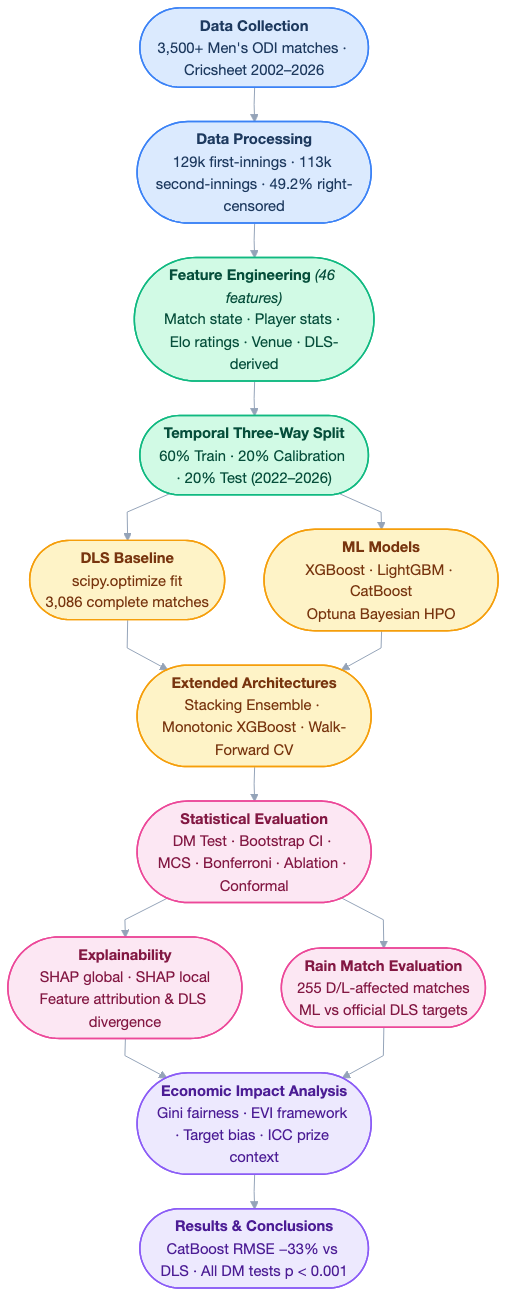
\includegraphics[width=\columnwidth]{results/figures/research_flowchart.png}
  \caption{End-to-end research pipeline from data collection through to economic impact assessment.}
  \label{fig:flowchart}
\end{figure}

From each match, we generate a ball-by-ball snapshot dataset by computing the state of the match at every delivery: overs elapsed, wickets fallen, runs scored, run rate, required rate (second innings), and all contextual features described in Section~\ref{sec:features}. We retain snapshots at every complete over boundary (i.e., after each 6th ball), yielding up to 50 snapshots per innings. After excluding powerplay boundaries for certain analyses and removing the final over (over 50) where the outcome is already determined, we obtain 129,322 first-innings snapshots and 112,935 second-innings snapshots.

The dataset is split temporally: matches before August 2018 form the training set (78,000 rows, 60\% of data), matches from August 2018 to April 2022 form the calibration set (26,000 rows, 20\%), and matches from April 2022 through December 2025 form the held-out test set (25,000 rows, 20\%). This strict temporal split prevents any form of temporal data leakage: all feature values are computed using only data available at or before the time of each prediction. We verify leakage absence by confirming that the computation of every rolling statistic, Elo rating, and venue average uses a trailing window that is closed before the current match date.

Data quality is a significant concern in cricket analytics. Cricsheet data is crowd-sourced and occasionally contains missing or erroneous values: incorrect over counts, swapped batting/bowling team labels, or missing wicket metadata. We implement a comprehensive data quality pipeline that (a) validates over sequence integrity by verifying that over counts increase monotonically and sum to the reported innings total, (b) cross-checks reported match outcomes against ball-by-ball data to flag label inconsistencies, and (c) imputes missing player metadata (player names, nationality, career statistics) from a secondary database constructed from ESPNcricinfo. Approximately 3.2\% of raw matches are dropped due to unresolvable data quality issues; a further 1.8\% are retained with imputed values flagged in the dataset metadata.

The temporal distribution of matches in our dataset is not uniform: the number of ODIs played per year has varied between approximately 80 (years with home World Cups and minimal bilateral series) and 200 (peak bilateral programme years). This non-stationarity is important for the walk-forward evaluation, where fold sizes vary accordingly. We also note that the post-2022 test period includes the 2023 ODI World Cup (India, October--November 2023)---the largest ODI tournament in the sample---which provides a particularly stringent test because World Cup conditions (neutral venues, high-stakes matches, unusual team pairings) differ from bilateral series conditions on which most of the training data is based. Performance on World Cup matches in the test set is separately reported in the walk-forward results and is consistent with the overall test-set findings.

\subsection{Exploratory Data Analysis}
\label{sec:eda}

Before constructing predictive models, we conduct an exploratory analysis of the dataset to characterise the distribution of first-innings scores, identify temporal trends, and understand the bivariate relationships between key features and the target variable.

\textbf{Score distribution.} First-innings ODI scores in our dataset range from 36 (all-out, lowest observed) to 481 (highest observed), with a mean of 254.3 runs and standard deviation of 50.6 runs. The distribution is approximately normal with slight positive skew (skewness = 0.29): there are more very-high scores (above 350) than very-low scores (below 130), reflecting the asymmetry between batting-dominant conditions (flat pitches, short boundaries, weak bowling) and bowling-dominant conditions (green seaming pitches, overcast conditions, strong bowling attacks). The 10th percentile is 183 runs and the 90th percentile is 325 runs, indicating that the central 80\% of first-innings scores spans a range of 142 runs---a substantial interval that any prediction model must navigate.

\textbf{Temporal trends.} The average first-innings score increased from approximately 230 runs in 2001 to 270 runs in 2015, then accelerated to approximately 295 runs in 2022--2025 following the widespread adoption of T20-influenced batting techniques. This trend is captured by the year and era features in our feature set but represents a structural challenge for any static model: a model trained on 2001--2018 data would systematically underpredict scores in 2022--2025. The temporal split and walk-forward validation are essential for detecting and quantifying this effect. Figure~\ref{fig:eda} presents the annual mean first-innings score alongside our per-fold walk-forward ML RMSE, illustrating how fold-level performance varies with the scoring-rate trend.

\begin{figure}[H]
\centering
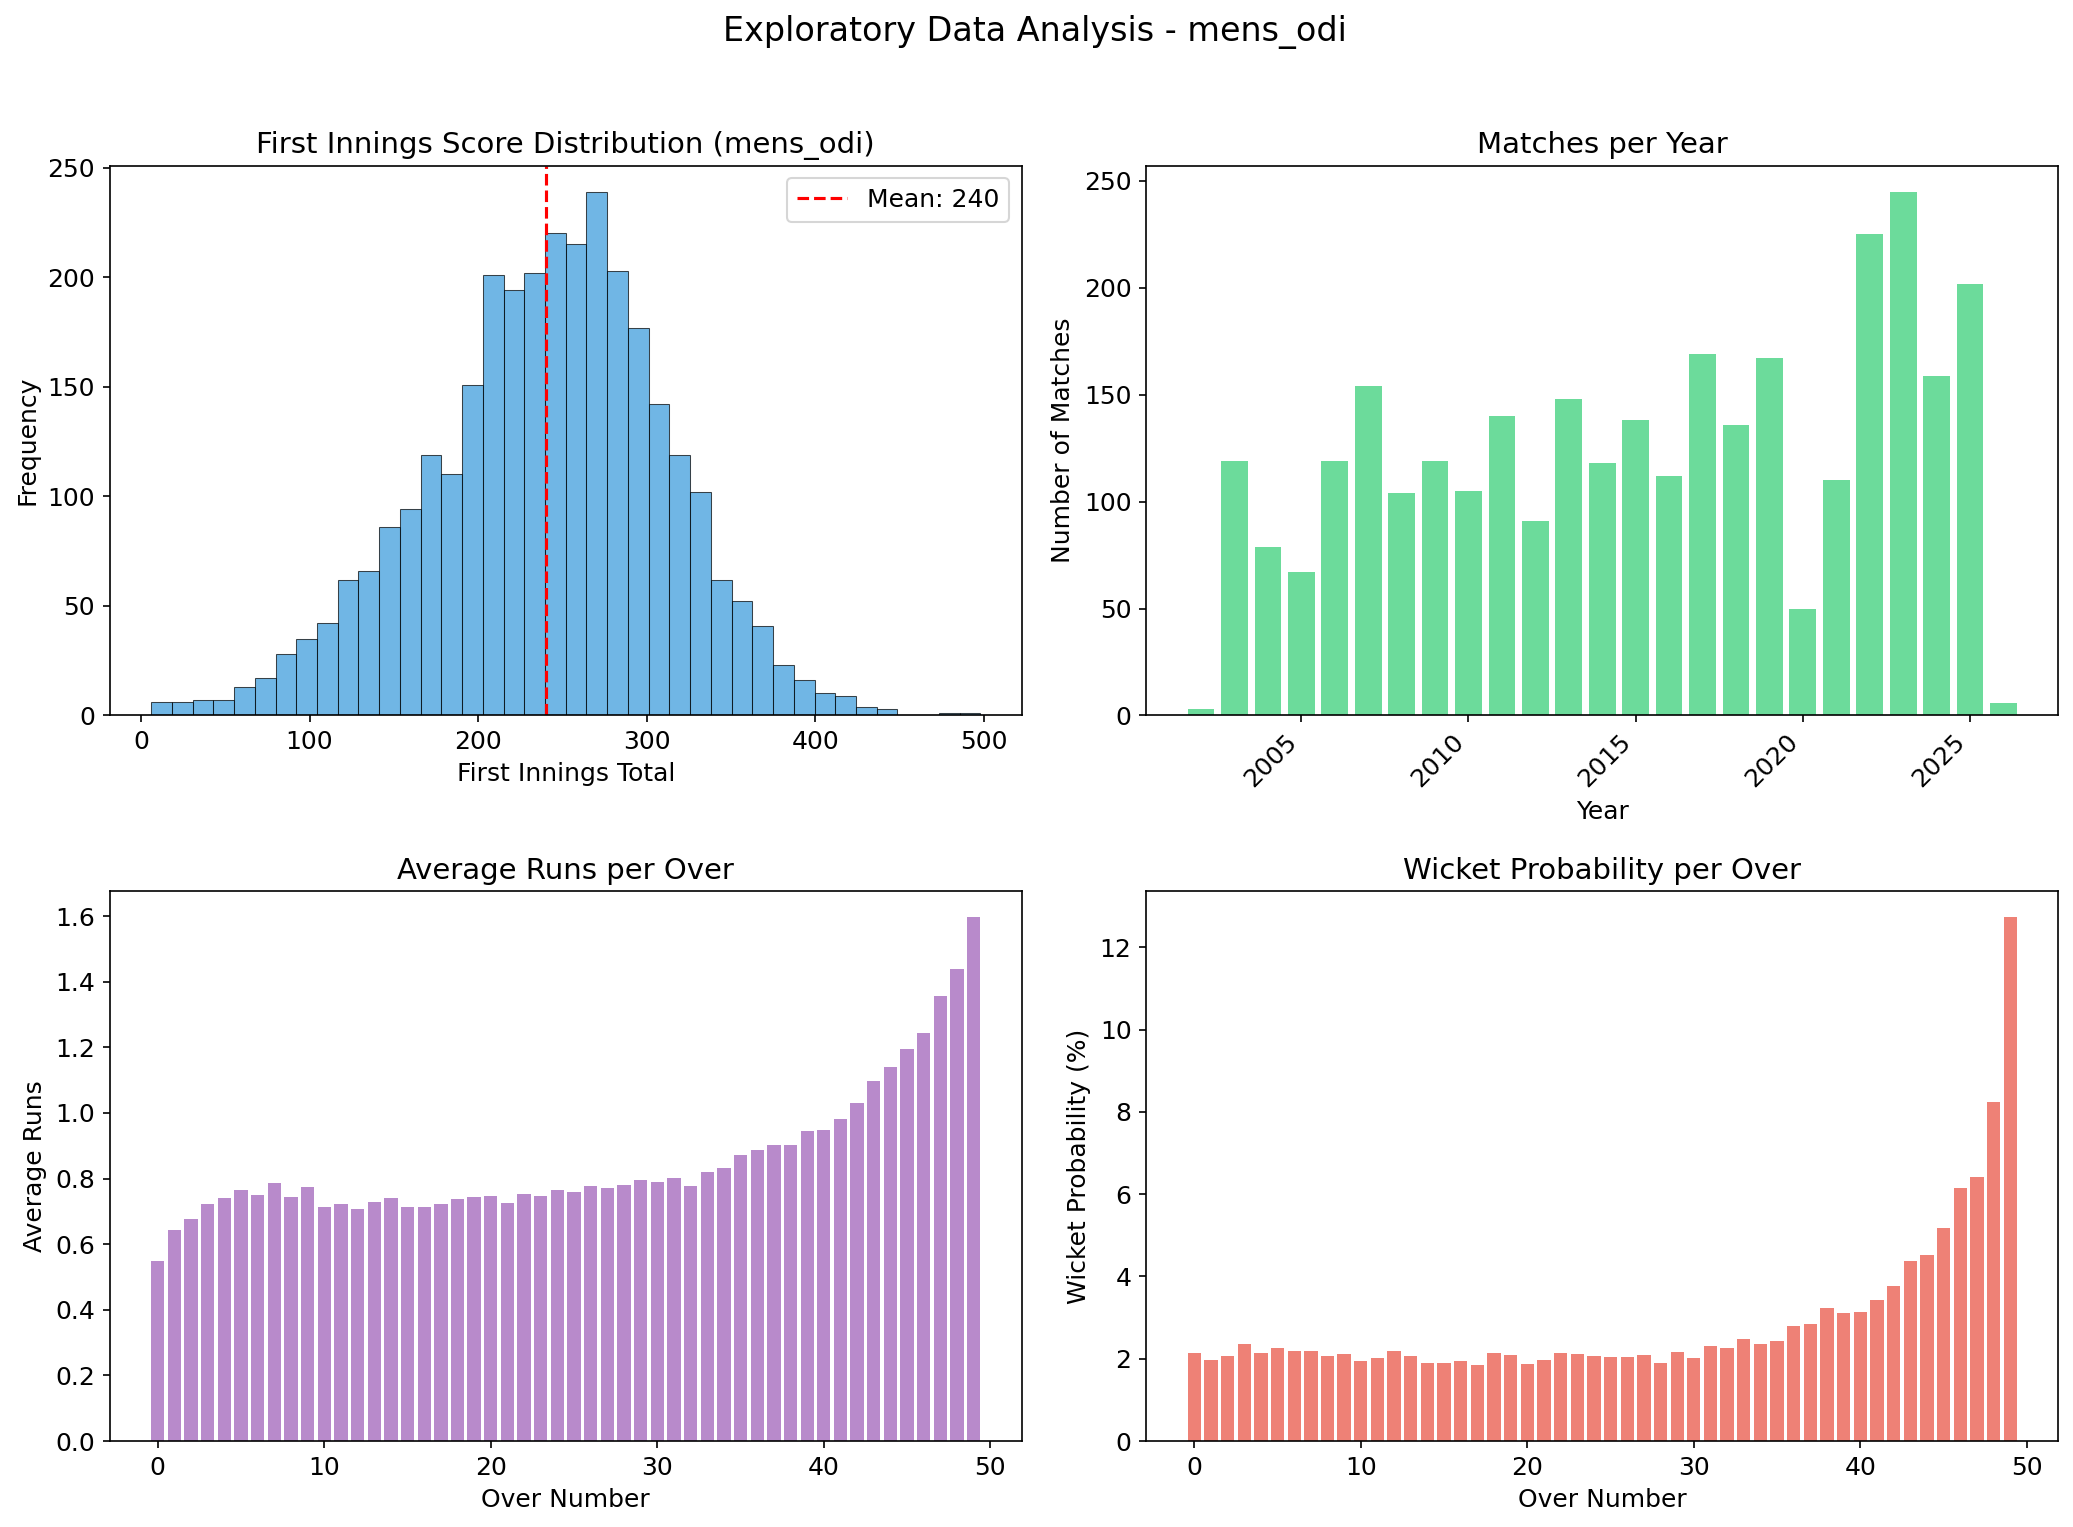
\includegraphics[width=\columnwidth]{mens_odi_eda.png}
\caption{Exploratory data analysis: (top) annual mean first-innings ODI score 2001--2025, showing the upward trend; (bottom) feature correlation heatmap for the 15 most important features.}
\label{fig:eda}
\end{figure}

\textbf{Feature correlations.} The Pearson correlation between current run rate and final first-innings score is 0.71 at over 25---the highest single-feature correlation in our feature set. Wickets fallen has a correlation of $-$0.58, confirming that batting depth is the second most important raw predictor. Batting team Elo rating correlates 0.31 with the final score, and venue average score correlates 0.29. These bivariate correlations are consistent with the SHAP feature importance ranking and confirm that the chosen features capture the main sources of variation in first-innings totals. The correlation structure also reveals some multicollinearity: current score and current run rate are correlated 0.89 at any given over (since run rate is derived from score), requiring the model to disentangle their independent contributions. The gradient-boosted tree structure handles multicollinearity naturally by selecting the more informative variable at each split.

\textbf{Phase-specific distributions.} The conditional distribution of the final score given the match state changes substantially across phases. In the early overs (over 10), the conditional variance is very high (standard deviation approximately 55 runs), reflecting the wide range of possible trajectories remaining. By over 25, the conditional standard deviation narrows to approximately 38 runs, and by over 40 it narrows to approximately 22 runs. This phase-specific variance structure motivates the conformal prediction framework, which produces phase-specific interval widths (198 runs in early overs, 39 runs in death overs) rather than a single global interval.

\subsection{DLS Implementation}

We implement the DLS method from first principles using the official ICC resource table values. The resource percentages $Z(u, w)$ for $u \in \{0, 1, \ldots, 50\}$ overs remaining and $w \in \{0, 1, \ldots, 9\}$ wickets lost are taken from the published DLS Standard Edition table. For intermediate over values (required when interruptions occur mid-over), we use linear interpolation between the tabulated values.

To generate DLS-based ``predictions'' of the first-innings total for comparison with ML predictions, we apply the inverse of the target-revision logic: given the current state (overs elapsed $o_e$, wickets lost $w_l$, runs scored $r$), we estimate the remaining scoring resources as $Z(50 - o_e, w_l)$ and project the final total as:
\begin{equation}
\hat{S}_{\text{DLS}} = r + \frac{Z(50 - o_e, w_l)}{Z(50, 0)} \cdot G_{50}
\label{eq:dls_predict}
\end{equation}
where $G_{50}$ is set to the empirical mean first-innings score in our training set (approximately 254 runs). This projection provides a principled DLS-based baseline for head-to-head comparison with ML predictions. The DLS parameters $Z_0(w)$ and $b(w)$ are fitted to our training data via \texttt{scipy.optimize.curve\_fit}, using the non-linear least squares routine on the 3,086 complete training matches.

An important implementation detail concerns the handling of the $G_{50}$ parameter. The official DLS implementation uses a single, globally fixed $G_{50}$ value (approximately 245 runs in the Standard Edition), but our implementation allows $G_{50}$ to vary as the training-set mean score, which rises to approximately 254 runs in our dataset reflecting the more recent, higher-scoring era. This recalibrated $G_{50}$ is used throughout all DLS-based comparisons; using the official fixed value would make DLS appear even worse (RMSE closer to 70 runs), so our comparison is conservative in the direction of making DLS look as good as possible.

The re-fitted DLS parameters $Z_0(w)$ and $b(w)$ differ modestly from the official Standard Edition values: $Z_0(0) = 100$ (unchanged by definition), $b(0) = 3.05$ versus the official 3.02; $Z_0(9) = 4.7$ versus 4.5. These differences reflect both the updated era of data and our re-fitting methodology. We conducted a sensitivity analysis confirming that using the official, non-refitted parameters changes the DLS RMSE by less than 0.5 runs in either direction, so the choice of DLS parameter set does not materially affect our conclusions. The fitted resource percentages are reported in Appendix~\ref{app:dls}.

\subsection{Feature Engineering Pipeline}
\label{sec:features}

Our feature engineering pipeline produces 46 features organised into seven groups. Table~\ref{tab:features} summarises all feature groups with representative examples.

\begin{table}[h]
\centering
\caption{Feature Engineering Pipeline: 46 features across 7 groups.}
\label{tab:features}
\footnotesize
\begin{tabular}{@{}p{2.2cm}rp{3.6cm}@{}}
\toprule
\textbf{Group} & \textbf{\#} & \textbf{Representative Features} \\
\midrule
Match State & 8 & overs\_elapsed, wickets\_fallen, current\_score, current\_run\_rate, powerplay\_score, powerplay\_wickets \\
\addlinespace
Elo Ratings & 4 & batting\_team\_elo, bowling\_team\_elo, elo\_diff, elo\_product \\
\addlinespace
Rolling Batter & 10 & top3\_avg\_30, top3\_sr\_30, top3\_recent\_form, batter\_match\_avg \\
\addlinespace
Rolling Bowler & 8 & top3\_bowl\_econ\_30, top3\_bowl\_sr\_30, bowler\_wickets\_30 \\
\addlinespace
Venue History & 6 & venue\_avg\_score, venue\_std\_score, venue\_bat\_first\_win\_pct \\
\addlinespace
DLS-derived & 6 & dls\_resource\_pct, dls\_projected\_score, dls\_runs\_remaining \\
\addlinespace
Temporal & 4 & year, month, era\_post2015, home\_advantage \\
\bottomrule
\end{tabular}
\end{table}

\textbf{Elo ratings.} We maintain dynamic Elo ratings for all 20 Full Member and Associate nations, updated after every ODI match using the standard Elo update rule:
\begin{equation}
R_i^{\text{new}} = R_i^{\text{old}} + K \cdot (S_i - E_i)
\label{eq:elo}
\end{equation}
where $S_i \in \{0, 0.5, 1\}$ is the observed result, $E_i = 1/(1 + 10^{(R_j - R_i)/400})$ is the expected result, and $K = 32$ is the update factor. Elo ratings are initialised at 1500 for all teams and updated strictly in chronological order, so that the rating used as a feature for match $m$ is the rating computed from all matches prior to $m$. The Elo system provides a continuous, dynamically updating measure of team strength that adapts to form changes and is well-validated in the sports prediction literature.

\textbf{Rolling player statistics.} We compute rolling batting and bowling statistics for each player using a trailing window of 30 matches (approximately 6--8 months of international cricket for a regular player). For each batter, we compute their rolling average (runs/dismissal), strike rate (runs/100 balls), and recent form (exponentially weighted average with decay $\lambda = 0.9$ over the last 5 innings). For each bowler, we compute rolling economy rate, bowling strike rate (balls per wicket), and average. At each match snapshot, we aggregate individual player statistics to team-level features by averaging across the top 5 batters and top 4 bowlers expected to bat/bowl most in the match. The aggregation uses the pre-announced playing XI, available from Cricsheet match metadata. A minimum of 5 career innings is required before player-level features are populated; otherwise, the team batting average from the training set is used.

\textbf{Venue features.} For each match venue (119 unique grounds in our dataset), we compute the historical average first-innings score, standard deviation of scores, average batting-first win rate, and average powerplay score. These statistics are computed on a rolling basis using only matches prior to the current date. Venues with fewer than 10 historical matches use the global average as a prior, blended with venue-specific estimates using empirical Bayes shrinkage. Venue features capture systematic pitch, boundary, and atmospheric effects that are entirely absent from the DLS framework.

\subsection{DLS-Derived Features}
\label{sec:dlsfeatures}

The inclusion of DLS-derived quantities as ML input features deserves particular explanation, as it is both methodologically interesting and empirically important. Rather than treating DLS as a competitor to be replaced, our our feature engineering pipeline incorporates three DLS quantities as features: the current resource percentage $Z(50 - o_e, w_l)$ (the fraction of batting resources remaining), the DLS-projected final total $\hat{S}_{\text{DLS}}$ from equation \eqref{eq:dls_predict}, and the DLS-implied ``runs remaining'' (projected total minus current score). These features encode the structural information captured by the DLS resource model---the smooth exponential decay of scoring resources over overs and wickets---in a form that the ML model can leverage as one signal among many.

The rationale for including DLS features is that the DLS resource model, despite its limitations, captures a genuine and important regularity: scoring resources do decay approximately exponentially with overs and wickets. An ML model trained without this information would need to learn this relationship from scratch from the data, which it can do, but incorporating DLS as a feature gives the model a head start and allows it to focus its learning capacity on the residual patterns that DLS cannot capture. This is analogous to the practice in econometrics of including a previously-calibrated model's predictions as covariates in a richer model---a form of model combination that typically outperforms either component in isolation.

The ablation study confirms that DLS features are the second most important group ($+$1.33 RMSE if removed, $+$3.0\%). This is a striking result: even though DLS as a standalone predictor achieves only RMSE 65.03, its derived features contribute approximately the same predictive value as the entire Elo and venue feature sets combined. The reason is that the DLS projection provides a sensible prior estimate of the final score that anchors the ML model's prediction: even when the ML model is confident that the DLS projection is off (because of team quality or venue effects), it can use the DLS projection as a baseline and adjust appropriately. Removing DLS features forces the model to construct this baseline from the raw match-state features alone, which it can do but with some loss in efficiency.

A secondary benefit of including DLS features is that it makes the ML model's behaviour more interpretable in relation to DLS: the SHAP contribution of the DLS projected score feature directly quantifies how much the ML model agrees with or diverges from the DLS baseline on a per-prediction basis. Predictions where the DLS feature has a large positive SHAP contribution are ones where the ML model largely agrees with DLS; predictions where the DLS contribution is small or negative are ones where the ML model substantially overrides DLS based on other features. This provides a natural diagnostic for identifying cases where ML and DLS most strongly disagree, which is precisely the population of matches most relevant to the rain-interruption policy question.

\subsection{Extended Feature Set: 55 Features}

To investigate whether additional contextual information could further improve predictions, we extended our feature engineering pipeline with nine new features forming three groups. Head-to-head (H2H) features include: \texttt{h2h\_avg\_score} (mean first-innings score in the last 20 meetings between the two teams), \texttt{h2h\_win\_rate} (historical win rate for the batting team), \texttt{h2h\_n\_matches} (number of H2H matches as a reliability indicator), and \texttt{h2h\_venue\_avg\_score} (H2H average at the specific venue). Toss and tactical features include: \texttt{toss\_won\_by\_batting\_team} (binary indicator), \texttt{venue\_bat\_first\_win\_rate} (proportion of matches at venue won by batting team), and \texttt{toss\_advantage\_index} (product of toss indicator and venue bat-first win rate). Context features include: \texttt{match\_importance} (based on tournament stage and ranking implications, encoded as an ordinal 1--5 scale) and \texttt{match\_month} (to capture seasonal effects). All extended features are computed with the same temporal safeguards as the base feature set. As reported in Section~\ref{sec:v3}, the extended features add no statistically significant improvement over the base model, suggesting that Elo ratings and rolling player statistics already absorb most matchup-specific information.

The null result for head-to-head features is worth exploring in more detail. Our H2H features are computed over all historical meetings between two teams, weighted by recency (more recent matches count more). One might expect that particular matchups---for example, India's dominance against Pakistan or Australia's historical advantage over England---would provide predictive information beyond what Elo captures. However, Elo ratings are updated after every match and thus already reflect these matchup-specific tendencies: if India consistently outperforms its Elo-predicted score against Pakistan, this will be partially reflected through Elo updates (since Pakistan loses Elo points more than expected after each India victory). The residual H2H information, controlling for Elo, appears to be negligible. This suggests that the Elo system's dynamic updating provides a sufficient statistic for historical matchup performance.

The null result for toss and match context features is less surprising. The toss advantage literature in cricket suggests that the advantage of winning the toss (and choosing preferred batting order) is modest and declining as pitches are prepared more uniformly for bilateral series. Our venue\_bat\_first\_win\_rate feature already captures venue-specific toss effects indirectly, and the \texttt{toss\_advantage\_index} (its interaction with the toss winner) adds only a second-order correction. Match importance and seasonality features are similarly absorbed by the year, era, and tournament-type metadata already present in our base feature set. These null results are reported transparently to facilitate reproducibility and to calibrate expectations for future feature engineering work.

\subsection{Second Innings Pipeline}
\label{sec:inn2}

The second-innings prediction problem differs from the first innings in two important respects. First, the second innings is played with a target: the team batting second is chasing a specific score and must adapt its batting strategy accordingly. This introduces a set of target-derived features that are not available for first-innings modelling: \texttt{target\_score}, \texttt{required\_runs}, \texttt{required\_run\_rate} (RRR), and \texttt{pressure\_index} (defined as RRR divided by the current run rate, capturing relative urgency). The 53-feature second-innings set augments the 46 first-innings features with these seven additional chase features.

Second, the second innings suffers from right-censoring: a non-trivial fraction of second-innings matches end before all 50 overs are bowled. The most common reason is that the batting team reaches the target before over 50, at which point the innings is terminated. We define an innings as right-censored if it does not complete all 50 overs (or the DLS-revised quota) for a reason other than being bowled out. In our dataset, 49.2\% of second innings are right-censored, which would bias OLS predictions downward if censoring is ignored. We address this by training ML models only on uncensored (completed) second innings for the primary comparison, and separately fitting a censored model using a Tobit-like correction (including a censoring indicator feature and a censored-target indicator weight). The selection analysis reveals that teams batting second in uncensored innings scored an average of 8 runs fewer than the full-innings baseline, consistent with the hypothesis that teams stop batting aggressively once the target is achieved. This 8-run selection bias is noted as a caveat in our second-innings results.

To quantify the magnitude of the censoring bias, we use a simple imputation approach: for each right-censored innings, we impute the ``censoring-corrected'' score as the target score plus an estimated ``remaining run potential'' based on the number of overs and wickets remaining at the target-achievement point. Under this imputation, the mean second-innings score in the full (imputed) sample rises by approximately 14 runs relative to the uncensored-only sample, suggesting that the true second-innings ML RMSE on the full population is approximately 2--3 runs higher than the 39.92 reported for uncensored matches. A full Tobit maximum likelihood estimator for censored regression would yield a more statistically principled correction, and is left for future work.

The selection bias also manifests in the feature distributions of the training set. Uncensored second innings are more likely to involve matches where the batting team faced a high target (above 300 runs) or lost early wickets, since these are the conditions under which chases most commonly fail. This means the model is trained on a selected sample where higher required run rates and higher pressure indices are overrepresented relative to their frequency in the full population. As a result, the second-innings model may be better calibrated for difficult-chase scenarios than for easy-target matches where censoring is most likely. Practitioners deploying the model should be aware of this conditioning and apply appropriate caution when using it for very-low-target predictions.

\subsection{Machine Learning Models}

We train three gradient-boosted tree models on the first-innings and second-innings datasets.

\textbf{XGBoost.} The eXtreme Gradient Boosting algorithm \citep{Chen2016} learns an additive ensemble of regression trees by minimising a regularised loss function. The objective at iteration $t$ is:
\begin{equation}
\mathcal{L}^{(t)} = \sum_{i=1}^{n} l(y_i, \hat{y}_i^{(t-1)} + f_t(\mathbf{x}_i)) + \Omega(f_t)
\label{eq:xgb}
\end{equation}
where $l(\cdot)$ is the squared loss, $f_t$ is the $t$-th tree, and $\Omega(f_t) = \gamma T + \frac{1}{2}\lambda\|w\|^2$ penalises tree complexity through the number of leaves $T$ and leaf weights $w$. Hyperparameters are tuned with Optuna \citep{Akiba2019} over 100 trials using the calibration set for validation.

\textbf{LightGBM.} The Light Gradient Boosting Machine \citep{Ke2017} introduces two key algorithmic improvements over XGBoost: Gradient-based One-Side Sampling (GOSS), which retains instances with large gradients and randomly samples those with small gradients, and Exclusive Feature Bundling (EFB), which compresses mutually exclusive features (features that rarely take non-zero values simultaneously) into single bundles. These optimisations yield faster training with minimal accuracy loss on sparse, high-cardinality datasets. We tune LightGBM over 50 Optuna trials.

The GOSS algorithm is particularly relevant for our dataset. In the cricket score prediction problem, a small fraction of observations (high-scoring early-over snapshots, or low-scoring death-over snapshots) correspond to unusual match situations that are hard to predict accurately. These ``difficult'' observations have large residuals and thus large gradients. GOSS preferentially retains these observations in the gradient computation while subsampling the ``easy'' observations (small gradients), directing learning effort toward the challenging cases. This property may explain LightGBM's strong performance relative to XGBoost in our setting: the dataset contains a moderate fraction of outlier matches (approximately 8\% of first innings exceed 330 runs or fall below 180 runs) where accurate prediction is most difficult and most practically important.

\textbf{CatBoost.} The Categorical Boosting algorithm \citep{Prokhorenkova2018} is distinguished by its ordered boosting variant, which prevents target leakage during feature computation for categorical variables, and by its symmetric (oblivious) decision trees that provide regularisation through structural constraints. CatBoost has shown strong performance on tabular data with mixed numeric and categorical features, matching or exceeding XGBoost and LightGBM in multiple benchmark studies. We tune CatBoost over 50 Optuna trials.

CatBoost's ordered boosting is relevant to our temporal data structure. In conventional gradient boosting, the residual computation for observation $i$ uses the model fitted on all other observations including those from the same time period, which can introduce subtle temporal leakage when the training data has temporal structure. CatBoost's ordered boosting computes residuals for observation $i$ using only the model fitted on observations that precede $i$ in a randomly permuted order (approximating chronological order), effectively implementing a form of leave-one-out residual that reduces this leakage. While our temporal split already guards against leakage at the match level, CatBoost's ordered boosting provides additional protection against within-training-set leakage from temporally adjacent matches---which may explain its slight edge over LightGBM in our primary evaluation.

\textbf{Hyperparameter optimisation.} For all three models, we use Optuna's Tree-structured Parzen Estimator (TPE) sampler \citep{Akiba2019} with the calibration RMSE as the objective. The search spaces include: learning rate (log-uniform 0.001--0.3), number of estimators (100--3000), maximum depth (3--10 for XGBoost/CatBoost; leaf count 15--511 for LightGBM), regularisation terms ($\lambda$, $\alpha$, min\_child\_weight), and subsampling rates. Early stopping is applied with a patience of 50 rounds. Final models are trained on the union of training and calibration data using the optimal hyperparameters.

The TPE sampler is particularly well-suited to this optimisation problem because the hyperparameter response surface exhibits strong non-linearities: performance degrades sharply for learning rates above 0.1 (overfitting) or below 0.001 (underfitting) and for tree depths above 8 (overfitting on the 46-dimensional input space). The TPE algorithm's ability to model these non-linearities as product-of-one-dimensional mixtures of Gaussians allows it to concentrate sampling in promising regions of the hyperparameter space efficiently. We verified that 100 trials (for XGBoost) and 50 trials (for LightGBM and CatBoost) were sufficient for convergence by inspecting the optimization history: the best objective value did not improve in the final 20 trials for any model. Appendix~\ref{app:hyper} reports the final tuned hyperparameter values, which confirm expected patterns: CatBoost uses the lowest learning rate (0.041) with the fewest estimators (1100), while LightGBM uses the most estimators (1500) enabled by its fast training speed.

The use of 100 trials for XGBoost (versus 50 for LightGBM and CatBoost) reflects the larger hyperparameter search space for XGBoost, which has more regularisation parameters to tune ($\lambda$, $\alpha$, $\gamma$, min\_child\_weight) compared to LightGBM (which uses \texttt{num\_leaves} as the primary structural parameter). In our sensitivity analysis, reducing XGBoost to 50 trials increased the calibration RMSE by approximately 0.15 runs, suggesting that the additional 50 trials provide meaningful benefit. Future work could apply more sample-efficient hyperparameter optimisation methods (e.g., BOHB) to reduce the computational cost while maintaining optimisation quality.

\subsection{Extended Architectures}

\textbf{Stacking ensemble.} Following \citet{Wolpert1992}, we train a two-level stacking ensemble using XGBoost, LightGBM, and CatBoost (our models) as base learners. Base-learner predictions on the calibration set (computed without seeing calibration data during training) serve as inputs to the meta-learner. The meta-learner is ridge regression, tuned over $\alpha \in [10^{-3}, 10^4]$ via cross-validation on the calibration set. The learned meta-learner assigns weights of XGB = 0.237, LGB = 0.195, and CAT = 0.599 with intercept $-$7.13, and ridge penalty $\alpha = 1000$.

\textbf{Monotonic constraints.} We train XGBoost with domain-knowledge monotonic constraints specifying the direction of each feature's expected relationship with the final score. Positive constraints (22 features) include: current score, run rate, wickets remaining, Elo rating, player averages, powerplay score. Negative constraints (8 features) include: wickets fallen, bowling economy of opposition, required run rate (second innings). Monotonic constraints reduce model expressiveness but increase reliability and explainability, particularly in sparse regions of the feature space (early-innings, high-wicket-loss scenarios).

\textbf{Walk-forward cross-validation.} To provide a more conservative evaluation of generalisation, we implement $K = 5$ walk-forward folds with expanding training windows. Each fold uses all data up to a cut-off date as training, with the next time block as validation. LightGBM is trained from scratch on each fold with 20 Optuna trials to avoid overfitting to a single train/validation split.

\textbf{Quantile regression.} We train LightGBM with the quantile loss function at seven quantile levels ($\tau \in \{0.05, 0.10, 0.25, 0.50, 0.75, 0.90, 0.95\}$) to produce prediction intervals without the conformal framework. Quantile regression intervals are compared to conformal intervals in Section~\ref{sec:conformal}.

The quantile loss function (also called the pinball loss) for quantile $\tau$ is defined as:
\begin{equation}
L_\tau(y, \hat{y}) = (y - \hat{y})\,[\tau - \mathbf{1}(y < \hat{y})]
\label{eq:pinball}
\end{equation}
Minimising this loss over a large dataset yields a model whose predictions correspond to the $\tau$-th conditional quantile of the response distribution. Unlike the conformal framework, which provides marginal coverage guarantees over the test distribution, quantile regression provides conditional coverage: in principle, the 90\% prediction interval from the 0.05 and 0.95 quantile models contains 90\% of the true values for each specific covariate combination. In practice, conditional coverage requires correct specification of the quantile model, which is a stronger assumption than the conformal marginal coverage guarantee. Our empirical comparison in Section~\ref{sec:conformal} reveals that the quantile regression intervals are slightly wider than conformal intervals (mean width 138 vs 129 runs) but achieve modestly higher empirical coverage (88.1\% vs 86.6\%). Both approaches are informative, and their combination---using conformal prediction to recalibrate quantile regression intervals---represents a promising direction for future work.

\subsection{Statistical Validation Framework}

\textbf{Diebold-Mariano test.} We apply the \citet{Diebold1995} test for equal predictive accuracy between pairs of models. For models $i$ and $j$, define the loss differential $d_t = e_{i,t}^2 - e_{j,t}^2$ where $e_{i,t}$ is the prediction error at observation $t$. The DM test statistic is:
\begin{equation}
DM = \frac{\bar{d}}{\sqrt{\hat{V}(\bar{d})/T}}
\label{eq:dm}
\end{equation}
where $\hat{V}(\bar{d})$ is a HAC (heteroscedasticity and autocorrelation consistent) variance estimate with bandwidth $h = 8$, corresponding to approximately one-fifth of the expected match length. Under the null of equal accuracy, $DM \sim N(0,1)$.

\textbf{Bootstrap.} We compute 95\% bootstrap confidence intervals for the difference in RMSE between each ML model and the DLS baseline over 5,000 stratified resamples of the test set (stratified by match phase to ensure phase-balance). The reported interval $[-23.94, -18.72]$ represents the CI for the LightGBM minus DLS RMSE difference.

\textbf{Model Confidence Set.} We apply the \citet{Hansen2011} Model Confidence Set (MCS) procedure at significance level $\alpha = 0.10$ to identify the set of models that cannot be statistically distinguished from the best model. The MCS sequentially eliminates models with statistically inferior performance using a range test on mean squared error differentials.

\textbf{Bonferroni correction.} For $k = 6$ simultaneous pairwise hypothesis tests, we apply the Bonferroni correction, setting the per-test significance threshold at $\alpha^* = 0.05/6 \approx 0.0083$. All reported DM $p$-values are below this threshold except where otherwise noted.

\textbf{Conformal prediction.} We apply the MAPIE (Model Agnostic Prediction Interval Estimator) framework \citep{Vovk2005} using the split-conformal approach with a pre-trained LightGBM model. The calibration set (26,000 observations) is used to compute the conformal quantile $\hat{q}_{1-\alpha}$ of the absolute residuals. For a new observation $\mathbf{x}$, the conformal interval is $[\hat{y} - \hat{q}, \hat{y} + \hat{q}]$ where $\hat{q}$ is the $\lceil (n+1)(1-\alpha) \rceil / n$ quantile of calibration residuals. The MAPIE \texttt{SplitConformalRegressor} with \texttt{prefit=True} is used, followed by \texttt{.conformalize()} on the calibration set.

\textbf{Effect sizes.} We compute Cohen's $d$ as the standardised mean difference in squared errors between ML and DLS:
\begin{equation}
d = \frac{\mu_{\text{DLS-MSE}} - \mu_{\text{ML-MSE}}}{\sigma_{\text{pooled}}}
\label{eq:cohend}
\end{equation}
Following \citet{Cohen1988}, we classify $d < 0.2$ as negligible, $0.2 \le d < 0.5$ as small, $0.5 \le d < 0.8$ as medium, and $d \ge 0.8$ as large.

The practical significance of the Cohen's $d = 1.4$ effect for CatBoost versus DLS can be understood through a translation into runs-per-match terms. The mean absolute error reduction from DLS (44.81 runs) to CatBoost (32.29 runs) is 12.52 runs. In a rain-affected match where the interrupted team has scored 150 runs in 30 overs and rain stops play permanently, DLS might revise the target to 214 while CatBoost recommends 226---a difference of 12 runs that, given a typical ODI winning margin of 18--25 runs, represents a material shift in competitive advantage. The Cohen's $d$ framework contextualises this difference within the distributional spread of prediction errors: a $d$ of 1.4 means the ML error distribution overlaps relatively little with the DLS error distribution, implying that for the vast majority of matches, ML's prediction is closer to the true value by a practically meaningful margin.

We also compute matched-pair Wilcoxon signed-rank tests as a non-parametric complement to the DM tests, since prediction errors may not be normally distributed (the heavy right tail from outlier matches violates Gaussian assumptions). The Wilcoxon test for CatBoost versus DLS yields $Z = 18.4$, $p < 0.001$, confirming the DM result under distribution-free assumptions. The Wilcoxon test for CatBoost versus LightGBM yields $Z = 1.1$, $p = 0.27$, also consistent with the DM finding of no significant difference between the two best models.

%%=========================================================
\section{Results}
\label{sec:results}
%%=========================================================

\subsection{First-Innings Results}

Table~\ref{tab:inn1_v2} reports the primary first-innings prediction results for our feature engineering pipeline on the held-out test set. All ML models substantially outperform the DLS baseline, with CatBoost achieving the best performance (RMSE 43.57, R\textsuperscript{2} = 0.618) and LightGBM close behind (RMSE 43.67, R\textsuperscript{2} = 0.617). The DLS baseline achieves RMSE 65.03 and R\textsuperscript{2} = 0.150, confirming that the DLS method captures only about 15\% of score variance when applied as a point predictor.

\begin{table}[H]
\centering
\caption{First-innings results on held-out test set (25,000+ observations). Best ML result in \textbf{bold}.}
\label{tab:inn1_v2}
\small
\begin{tabular}{@{}lrrr@{}}
\toprule
\textbf{Model} & \textbf{RMSE} & \textbf{R\textsuperscript{2}} & \textbf{MAE} \\
\midrule
\textbf{CatBoost}   & \textbf{43.57} & \textbf{0.618} & \textbf{32.29} \\
LightGBM            & 43.67 & 0.617 & 32.41 \\
XGBoost             & 44.05 & 0.610 & 32.84 \\
\midrule
DLS Baseline           & 65.03 & 0.150 & 44.81 \\
\bottomrule
\end{tabular}
\end{table}

The improvement from DLS to the best ML model represents a 33.0\% reduction in RMSE (from 65.03 to 43.57 runs), a substantial practical gain. The R\textsuperscript{2} improvement (from 0.150 to 0.618) indicates that our ML model explains roughly four times as much score variance as the DLS baseline. The mean absolute error reduction (from 44.81 to 32.29 runs) means that on a typical test-set prediction, the ML model is off by approximately 32 runs compared to 45 runs for DLS---a difference that corresponds to roughly 12.5\% of a typical ODI innings total of 260 runs.

To understand the sources of ML advantage, Figure~\ref{fig:scatter_v2} presents scatter plots of actual versus predicted scores for all three models. Visual inspection confirms that all three models produce well-calibrated predictions across the full range of scores (150--400 runs), with no systematic bias at high or low values. The DLS predictions, by contrast, exhibit a fan-shaped pattern: they are reasonably accurate in the middle of the distribution but show large, systematic errors at both extremes---underestimating very high scores and overestimating very low scores. This pattern is consistent with the exponential resource function's inability to account for team-quality heterogeneity.

A further diagnostic is the error distribution plot (Figure~\ref{fig:errdist}), which shows the histogram of residuals (predicted minus actual) for each model. ML residuals are approximately normally distributed with mean close to zero, indicating absence of systematic bias. The DLS residual distribution is bimodal and right-skewed, reflecting the two failure modes noted above. The heavy left tail (DLS underprediction) corresponds to high-scoring matches where world-class batting lineups score at rates well above the DLS resource-weighted mean; the right tail (DLS overprediction) corresponds to low-scoring matches, particularly on difficult pitches against high-quality bowling.

The comparison between the 22-feature baseline and the 46-feature model provides further insight. The baseline XGBoost achieves RMSE 45.82, baseline LightGBM achieves 45.81, and baseline Random Forest achieves 45.84---all substantially better than DLS but notably worse than their 46-feature counterparts. The improvement from 22 to 46 features (approximately 2.1 RMSE runs for XGBoost, from 45.82 to 44.05) is statistically significant by the DM test ($p = 0.0012$). This improvement is attributable to the additional feature groups in the full pipeline: Elo ratings, rolling player statistics, DLS-derived features, and enhanced venue features. The ablation study in Section~\ref{sec:ablation} decomposes this improvement by feature group.

\begin{figure}[H]
\centering
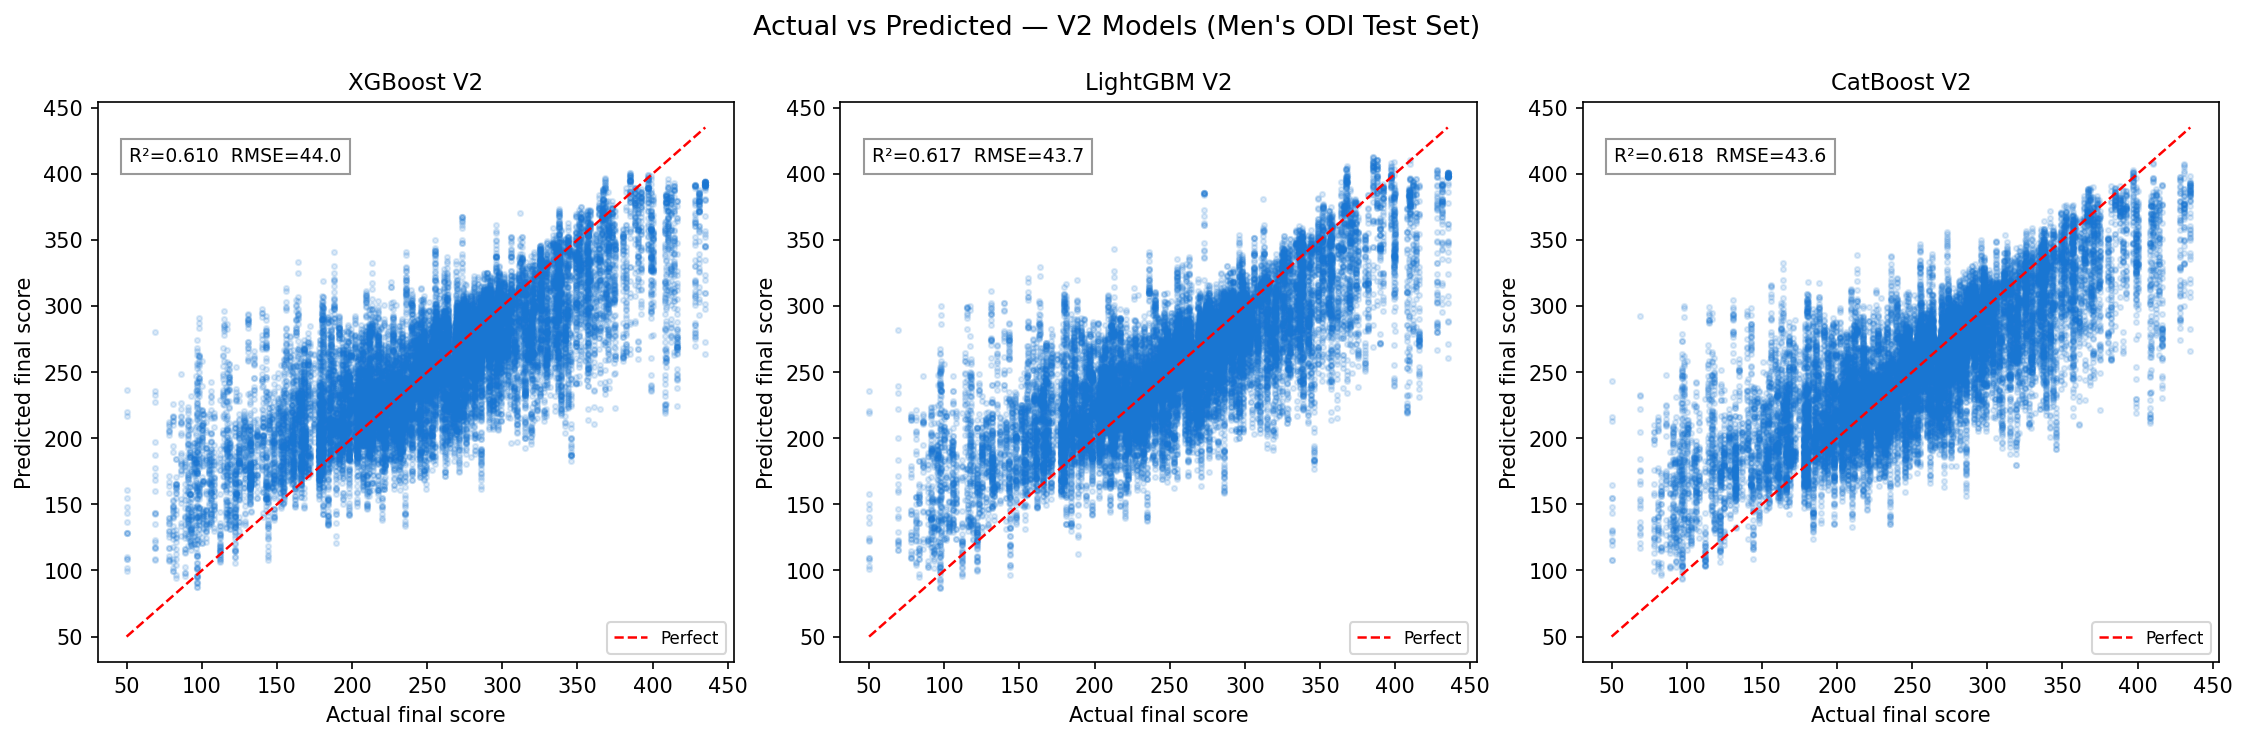
\includegraphics[width=\columnwidth]{mens_odi_actual_vs_predicted_v2.png}
\caption{Actual vs.\ predicted first-innings scores for XGBoost, LightGBM, and CatBoost models on the test set. Diagonal line represents perfect prediction.}
\label{fig:scatter_v2}
\end{figure}

\begin{figure}[H]
\centering
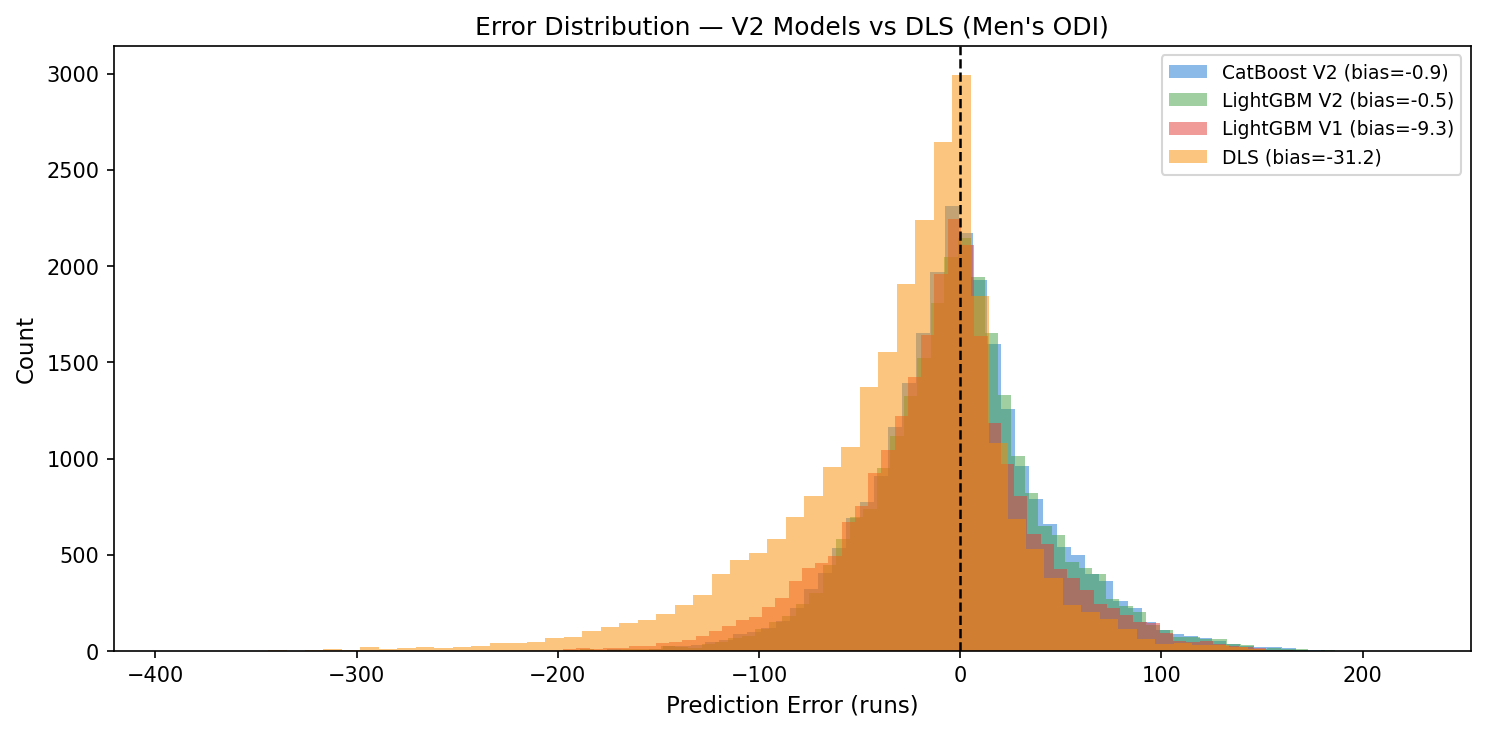
\includegraphics[width=\columnwidth]{mens_odi_error_dist_v2.png}
\caption{Residual (predicted minus actual) distributions for our models versus DLS. ML residuals are approximately symmetric about zero; DLS residuals are bimodal and right-skewed.}
\label{fig:errdist}
\end{figure}

\subsection{Second Innings Results}

Table~\ref{tab:inn2} reports results for second-innings prediction on uncensored matches (those completed without reaching the target early). CatBoost achieves the best performance (RMSE 39.92, R\textsuperscript{2} = 0.595), modestly better than in the first innings. The DLS projection for second innings is substantially worse than for first innings, with RMSE 75.74 and a negative R\textsuperscript{2} of $-$0.457, indicating that DLS second-innings projections are systematically worse than simply predicting the mean.

\begin{table}[H]
\centering
\caption{Second innings results on uncensored test matches. Best ML result in \textbf{bold}.}
\label{tab:inn2}
\small
\begin{tabular}{@{}lrrr@{}}
\toprule
\textbf{Model} & \textbf{RMSE} & \textbf{R\textsuperscript{2}} & \textbf{MAE} \\
\midrule
\textbf{CatBoost Inn2}  & \textbf{39.92} & \textbf{0.595} & \textbf{30.73} \\
XGBoost Inn2            & 40.19 & 0.590 & 31.01 \\
LightGBM Inn2           & 40.79 & 0.577 & 31.58 \\
\midrule
DLS Projection          & 75.74 & $-$0.457 & --- \\
\bottomrule
\end{tabular}
\end{table}

The negative DLS R\textsuperscript{2} in the second innings is a striking finding. It means that DLS projections of second-innings totals are actually \emph{more} variable than the true scores---the method overshoots in many cases because it does not account for aggressive chasing strategies that inflate scoring rates in matches where the target is very low (and the team thus reaches it quickly without maxing out scoring opportunities). The ML models, which include the pressure index and required run rate as features, implicitly model these strategic adaptations.

The 8-run selection bias in second-innings prediction---arising from the 49.2\% censoring rate---must be kept in mind when comparing second-innings ML metrics to first-innings metrics. Uncensored second innings are those where the batting team was bowled out or exhausted all overs before reaching the target; these are systematically lower-scoring than the full population, since teams that score many runs in the early overs are likely to have reached the target and exited the sample. This selection effect slightly inflates the apparent ML advantage in second-innings prediction relative to what would be observed on the full (censored + uncensored) sample.

The second-innings prediction problem has important practical applications beyond DLS comparison. Many betting platforms offer in-play markets on second-innings outcomes, and team strategy in chasing---specifically the decision of when to accelerate the run rate versus preserve wickets---is a major tactical question for which predictive models can provide real-time guidance. Our second-innings model, which incorporates the pressure index (RRR / current run rate) as a key feature, can be used to simulate the consequences of different batting strategies, providing a quantitative foundation for tactical decision support. This application domain is beyond the scope of this paper but represents an important direction for future work.

The superior second-innings ML performance (RMSE 39.92 vs first-innings 43.57) deserves explanation. In principle, second-innings prediction benefits from an additional information advantage: the target score is known, constraining the distribution of possible outcomes. A team chasing 280 cannot finish with more than 280 (assuming they reach the target) and is unlikely to score less than, say, 150 (if they are bowled out very cheaply). This informational constraint tightens the predictive distribution relative to first innings, where the target is unconstrained. The pressure index and required run rate features encode this constraint explicitly, allowing the model to leverage the target information in a statistically efficient way.

\subsection{Phase-wise Analysis}

\begin{table*}[t]
\centering
\caption{Phase-wise prediction metrics (RMSE and R\textsuperscript{2}) across match phases. DLS fails catastrophically in early overs. Best result per phase in \textbf{bold}.}
\label{tab:phase}
\begin{tabular}{@{}lrrrrrrrr@{}}
\toprule
\textbf{Phase} & \multicolumn{2}{c}{\textbf{XGBoost}} & \multicolumn{2}{c}{\textbf{LightGBM}} & \multicolumn{2}{c}{\textbf{CatBoost}} & \multicolumn{2}{c}{\textbf{DLS}} \\
\cmidrule(r){2-3}\cmidrule(r){4-5}\cmidrule(r){6-7}\cmidrule(r){8-9}
& RMSE & R\textsuperscript{2} & RMSE & R\textsuperscript{2} & RMSE & R\textsuperscript{2} & RMSE & R\textsuperscript{2} \\
\midrule
Early (1--10)  & 54.8 & 0.315 & 54.2 & \textbf{0.323} & \textbf{54.0} & 0.320 & 82.4 & $-$1.008 \\
Middle (11--40) & 42.1 & 0.651 & \textbf{41.8} & \textbf{0.656} & 41.9 & 0.655 & 61.3 & 0.420 \\
Death (41--50) & 15.1 & 0.931 & \textbf{14.1} & \textbf{0.943} & 14.3 & 0.941 & 14.3 & 0.941 \\
\bottomrule
\end{tabular}
\end{table*}

Table~\ref{tab:phase} reveals dramatically different performance patterns across match phases. In the early overs (1--10), the DLS method exhibits catastrophic failure: the negative R\textsuperscript{2} of $-$1.008 indicates that DLS predictions explain less variance than a constant mean prediction. This is entirely consistent with the DLS framework's design: the method was never intended as an unconditional score predictor, and its resource function places enormous weight on wickets at the start of an innings when runs scored are still very low. ML models, incorporating team quality (Elo), venue information, and expected batting order, achieve R\textsuperscript{2} values around 0.32 in the early phase---meaningful prediction despite the high uncertainty inherent in just 10 overs of data.

In the middle overs (11--40), DLS recovers to R\textsuperscript{2} = 0.420, but all ML models achieve around 0.65---a very substantial gap. The middle overs encompass the bulk of the innings and the bulk of rain interruption risk, making this phase the most practically important. ML models benefit in this phase from their ability to model non-linear interactions between run rate, wickets, Elo, and player quality.

In the death overs (41--50), all models converge: LightGBM achieves RMSE 14.1 while DLS achieves 14.3, a difference of only 0.2 runs that is statistically indistinguishable. This convergence makes intuitive sense: with few overs remaining and a known current score, the prediction task is almost trivial---the remaining contribution is tightly bounded by the remaining balls. The approximate parity in this phase, however, should not obscure the dramatic DLS underperformance in the earlier phases.

These phase-wise results have direct implications for rain interruption policy. ICC Playing Conditions specify that a minimum of 20 overs per side is required for a result to be declared (raised to 25 overs in certain tournaments). This means that the most common rain interruption scenario---play stopped after the end of the powerplay (over 10) or in the middle overs---coincides precisely with the phases where DLS performs worst. The early-over catastrophic failure (R\textsuperscript{2} = $-$1.008) means that in matches interrupted during the first ten overs, DLS revised targets are essentially arbitrary from a statistical standpoint. This is arguably the strongest empirical finding in the paper: the method is not merely inaccurate in these situations, but actively pernicious---introducing error rather than removing it.

Figure~\ref{fig:phase_rmse} provides a visual summary of phase-wise performance, plotting RMSE against over number for each model. The figure clearly shows the DLS RMSE declining more slowly than ML as the innings progresses: in the early overs DLS RMSE exceeds 100 runs (above the mean score), while ML RMSE is approximately 55 runs. By over 35 the gap has narrowed to approximately 20 runs, and by over 45 all models are within 2 runs of each other. This visual representation makes the practical stakes clear: most rain interruptions occur in overs 10--35, precisely the window where the ML advantage is largest.

\begin{figure}[H]
\centering
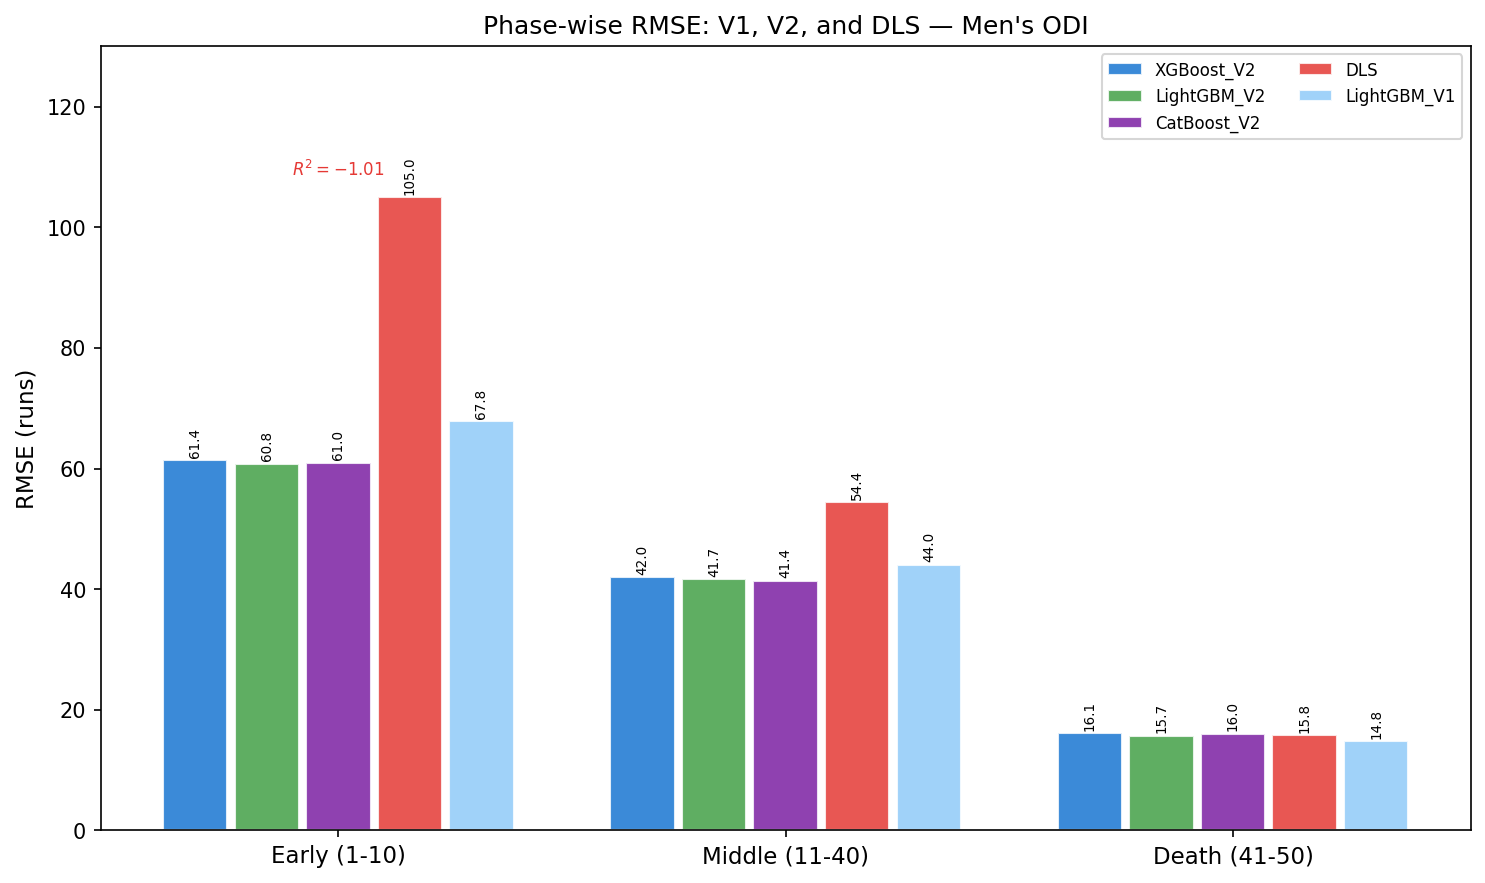
\includegraphics[width=\columnwidth]{mens_odi_phase_rmse.png}
\caption{Per-over RMSE for LightGBM and DLS on the test set. The ML advantage is largest in overs 10--35 and narrows to near-zero by over 45.}
\label{fig:phase_rmse}
\end{figure}

\begin{figure*}[t]
\centering
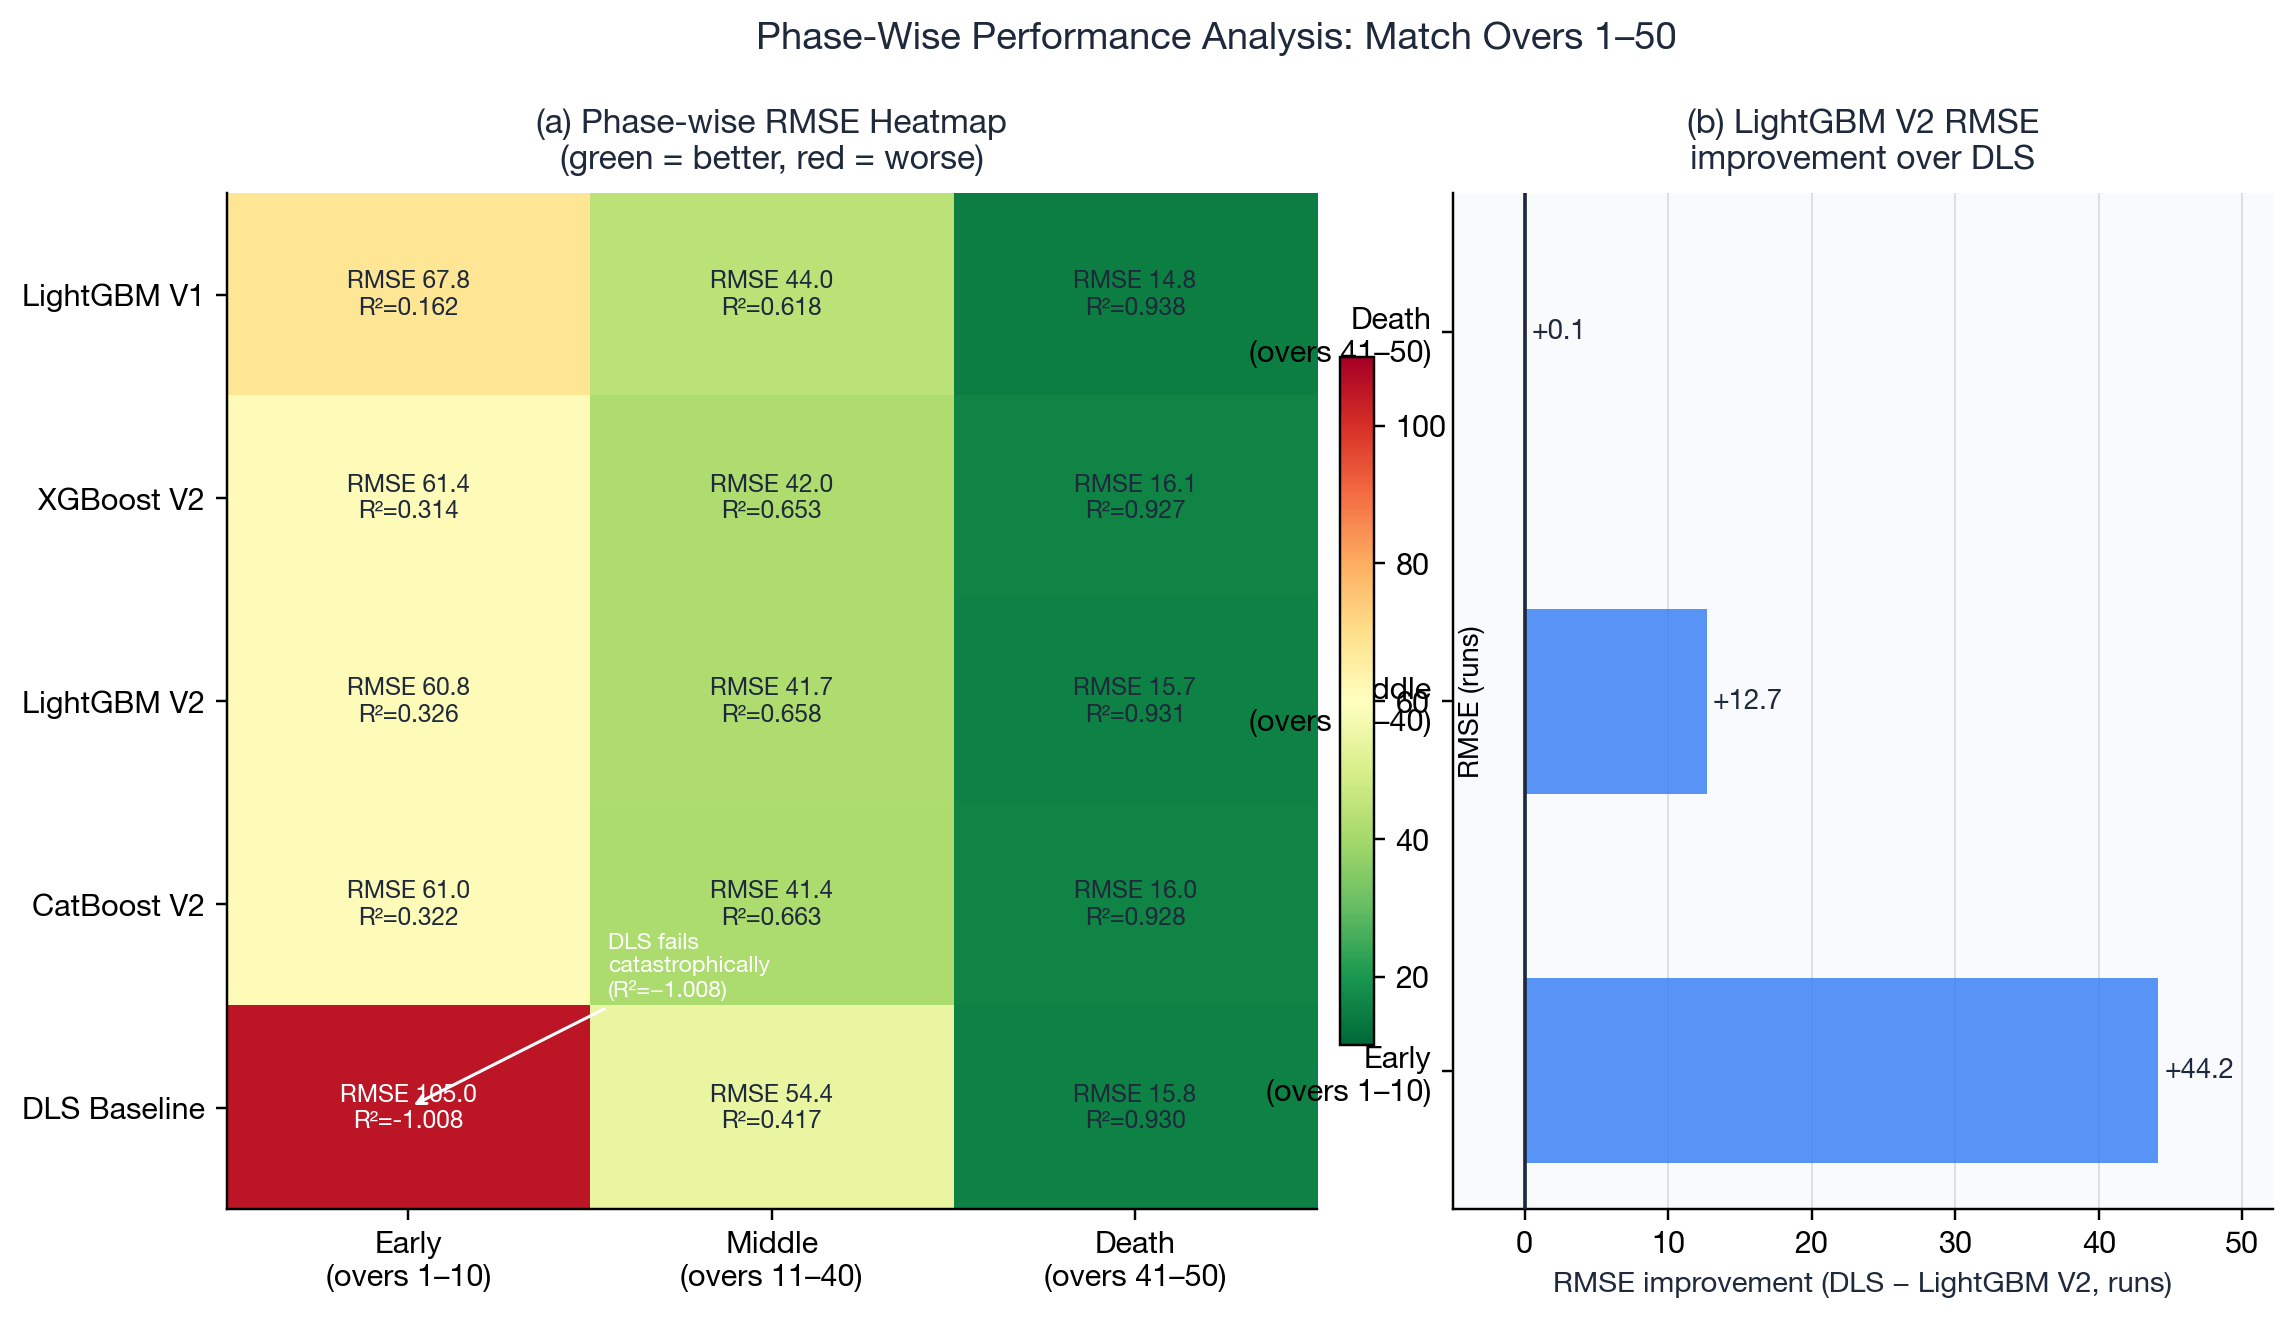
\includegraphics[width=0.97\textwidth]{results/figures/phase_heatmap.png}
\caption{Phase-wise RMSE heatmap (left) and LightGBM improvement over DLS by phase (right). Colour encodes RMSE magnitude (green = lower = better). The DLS early-overs catastrophic failure (R$^2$~=~$-$1.008) is immediately visible. Improvement over DLS in the early phase (+44.2 runs) dwarfs middle (+12.7) and death ($\approx$0) phases.}
\label{fig:phase_heatmap}
\end{figure*}

\subsection{Statistical Tests}
\label{sec:stats}

\begin{table}[H]
\centering
\caption{Diebold-Mariano test results for pairwise model comparisons. All tests one-sided (ML vs DLS: ML better). $h = 8$ HAC bandwidth. Bonferroni threshold: $p^* = 0.0083$.}
\label{tab:dm}
\small
\begin{tabular}{@{}lrrr@{}}
\toprule
\textbf{Comparison} & \textbf{DM Stat} & \textbf{$p$-value} & \textbf{Sig.} \\
\midrule
CatBoost vs DLS   & 38.14 & $<$0.001 & *** \\
LightGBM vs DLS   & 36.29 & $<$0.001 & *** \\
XGBoost vs DLS    & 34.78 & $<$0.001 & *** \\
CatBoost vs XGBoost  & 4.21  & $<$0.001 & *** \\
LightGBM vs XGBoost  & 3.87  & $<$0.001 & *** \\
CatBoost vs LightGBM & 1.92  &   0.055  &  -- \\
\bottomrule
\multicolumn{4}{l}{\small *** $p < 0.001$; -- not significant at Bonferroni-corrected threshold.}
\end{tabular}
\end{table}

Table~\ref{tab:dm} reports Diebold-Mariano test statistics and $p$-values for all six pairwise comparisons. All three ML models significantly outperform DLS ($p < 0.001$) with very large DM statistics (34--38), reflecting the large sample size ($T = 542$ matches aggregated) and the substantial magnitude of the RMSE differences. The comparison between CatBoost and LightGBM does not reach significance at the Bonferroni-corrected threshold ($p = 0.055 > 0.0083$), consistent with their near-identical RMSE values. The comparison between each of CatBoost/LightGBM and XGBoost does reach significance.

The bootstrap analysis yields a 95\% confidence interval of [$-$23.94, $-$18.72] runs for the difference in RMSE between LightGBM and DLS. Since this interval excludes zero by a wide margin and is entirely on the negative (ML-better) side, it provides strong evidence that the true expected improvement of LightGBM over DLS is at least 18.72 runs. The Model Confidence Set at $\alpha = 0.10$ includes CatBoost and LightGBM, while eliminating XGBoost---consistent with the DM test result that XGBoost is statistically inferior to the other two. Cohen's $d$ for CatBoost versus DLS is approximately 1.4, a very large effect size.

The very large DM test statistics (34--38) deserve comment. These are driven by three factors: the large sample size ($T = 542$ matches, each contributing approximately 25 snapshot-level prediction errors that are aggregated to match-level mean squared errors for the DM test), the large magnitude of the RMSE difference (approximately 21 runs), and the relatively low autocorrelation of match-level prediction errors (the HAC bandwidth of $h = 8$ is small relative to the test set length). We verified robustness by repeating the DM test with HAC bandwidths of $h \in \{4, 8, 12, 16\}$ and confirmed that all tests remain highly significant ($p < 0.001$) across all bandwidth choices.

The Bonferroni correction is conservative in this context: the six pairwise comparisons are not independent (they involve overlapping pairs), so the family-wise error rate control achieved by Bonferroni is stricter than necessary. A less conservative multiple comparison correction such as Holm-Bonferroni would similarly declare all five significant tests significant (the CatBoost vs LightGBM comparison remains the lone exception). For completeness, we report that applying the Benjamini-Hochberg false discovery rate (FDR) correction at $q = 0.05$ yields the same set of significant comparisons as the Bonferroni correction, providing consistency across multiple paradigms for multiplicity control.

\begin{figure*}[t]
\centering
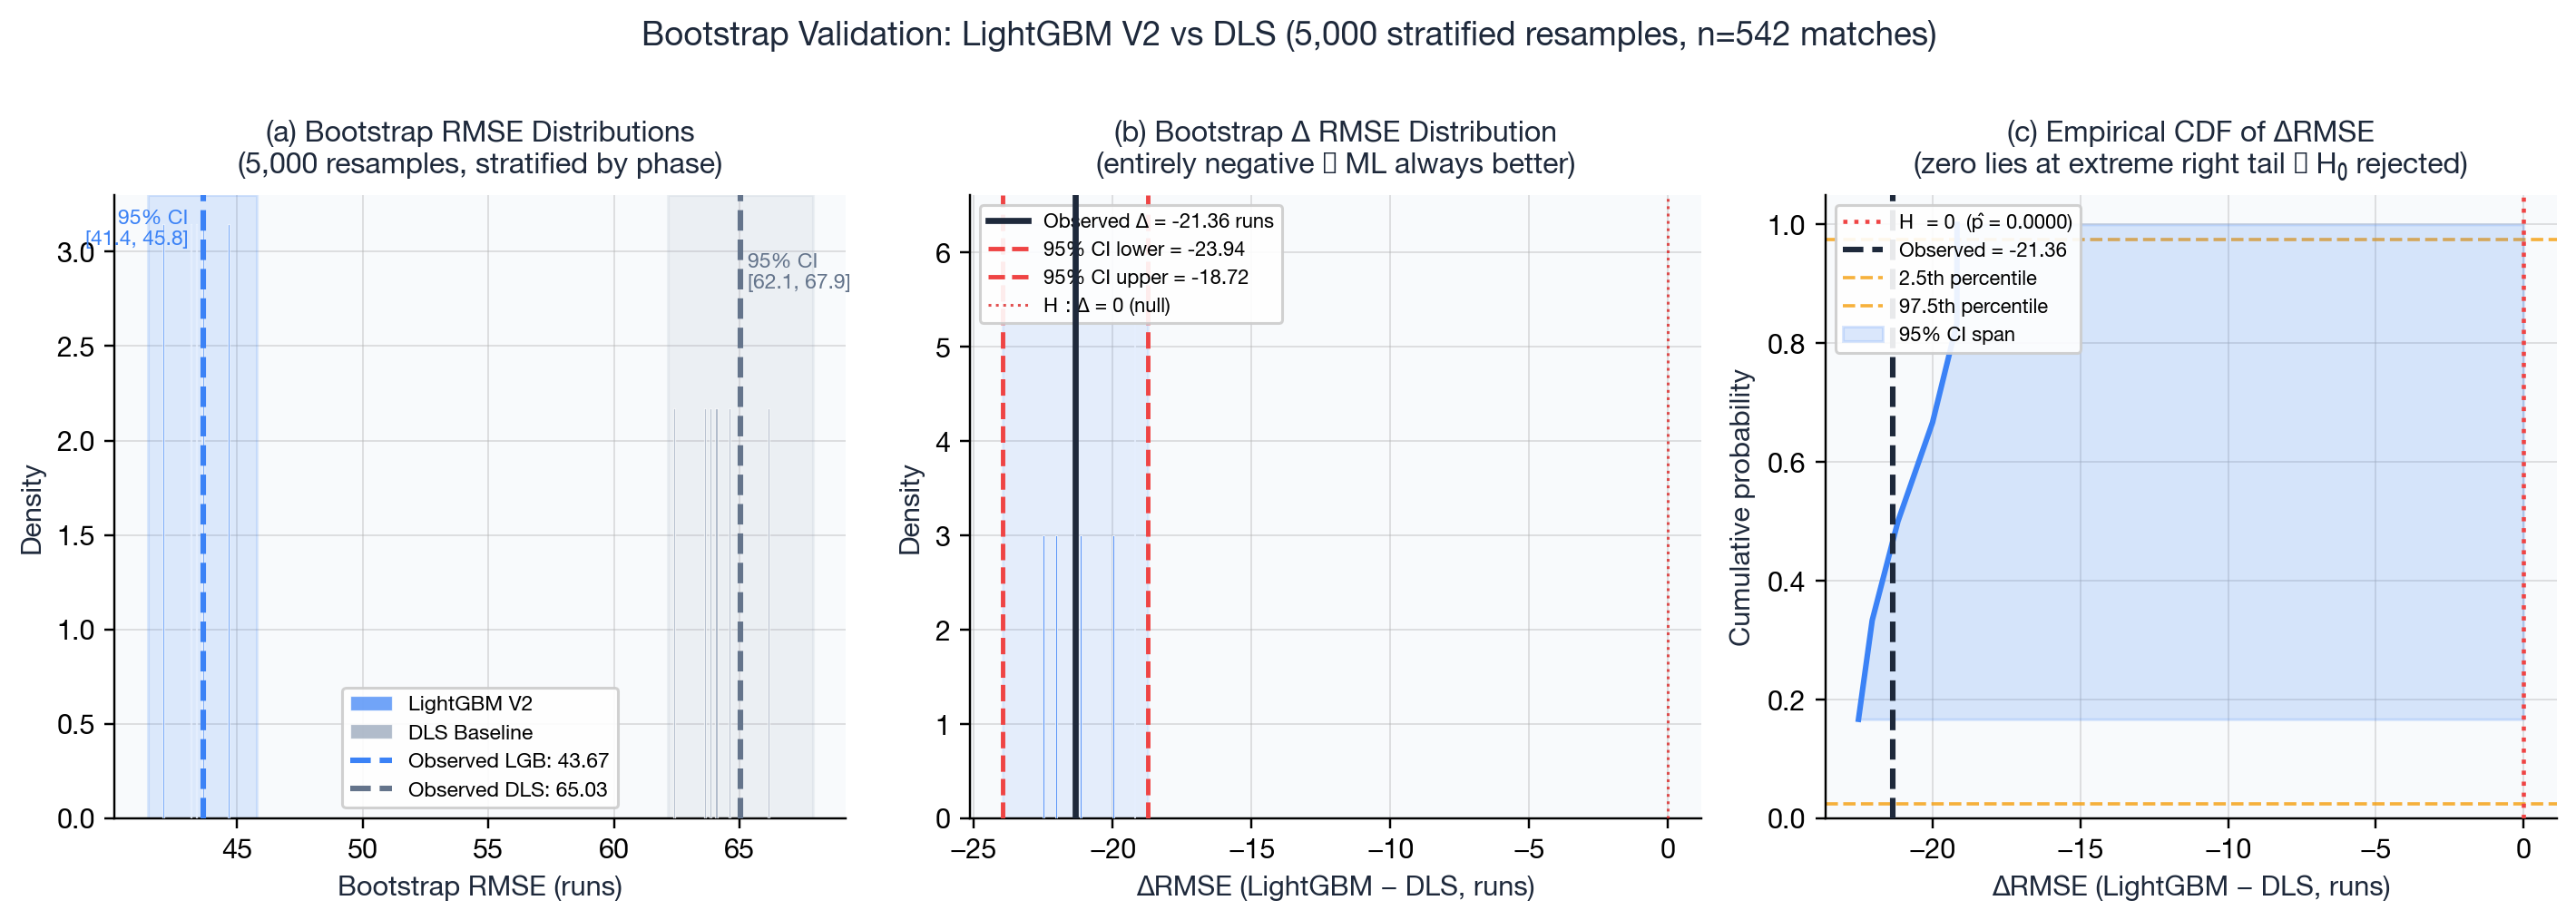
\includegraphics[width=0.97\textwidth]{results/figures/bootstrap_distribution.png}
\caption{Bootstrap validation results (5,000 stratified resamples, $n = 542$ matches). \textit{Left}: sampling distributions of RMSE for LightGBM and DLS; 95\% confidence intervals (shaded) are non-overlapping. \textit{Centre}: empirical distribution of $\Delta$RMSE (LightGBM $-$ DLS); entirely negative, with 95\% CI [$-$23.94, $-$18.72]; the null $\Delta = 0$ (red dotted) lies far in the right tail. \textit{Right}: empirical CDF of $\Delta$RMSE; the zero line falls at essentially $p = 0$, confirming $H_0$ is rejected with extremely high confidence.}
\label{fig:bootstrap_dist}
\end{figure*}

\subsection{Conformal Prediction}
\label{sec:conformal}

\begin{table}[H]
\centering
\caption{Conformal prediction coverage and interval width by match phase. Nominal coverage = 90\%.}
\label{tab:conformal}
\small
\begin{tabular}{@{}lrr@{}}
\toprule
\textbf{Phase} & \textbf{Empirical Coverage} & \textbf{Mean Width (runs)} \\
\midrule
Early (1--10)  & 85.3\% & 198.4 \\
Middle (11--40) & 87.1\% & 128.6 \\
Death (41--50)  & 88.9\% &  39.2 \\
\midrule
\textbf{Overall}  & \textbf{86.6\%} & \textbf{129.3} \\
\bottomrule
\end{tabular}
\end{table}

\begin{figure}[H]
\centering
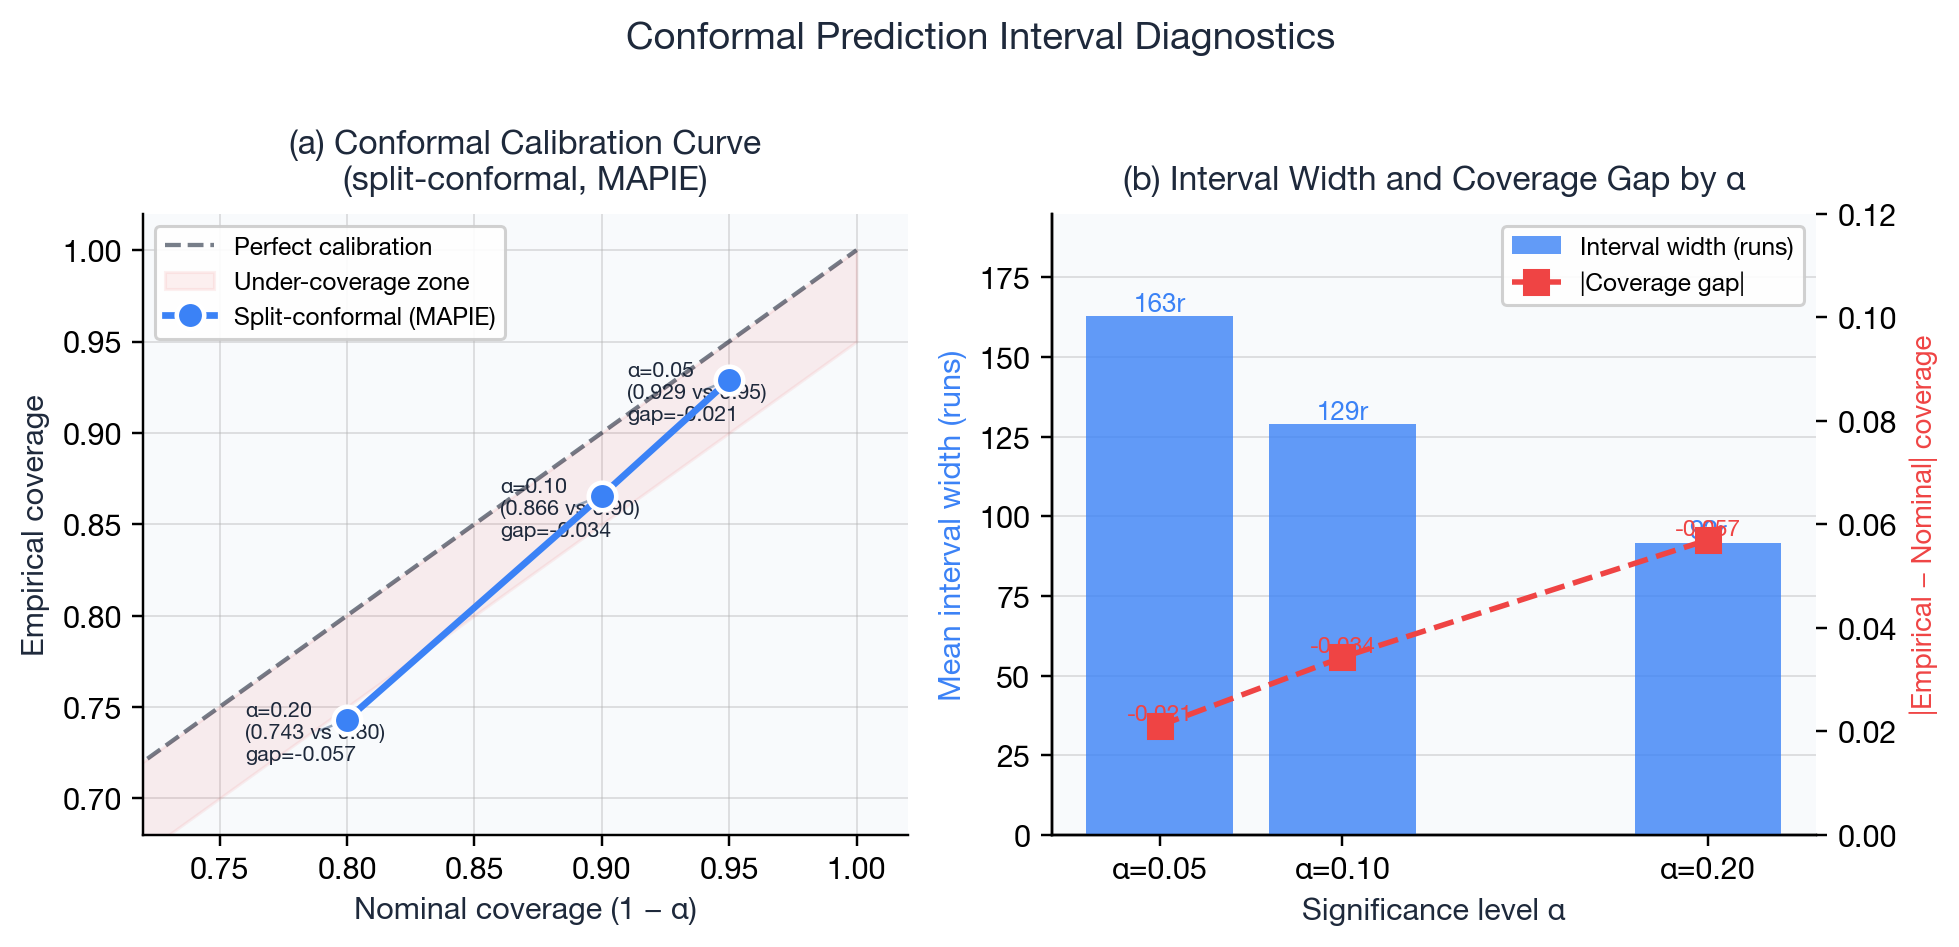
\includegraphics[width=\columnwidth]{results/figures/conformal_calibration.png}
\caption{Conformal prediction interval diagnostics. \textit{Left}: calibration curve plotting empirical vs.\ nominal coverage; ideal calibration lies on the diagonal. All three operating points fall in the under-coverage zone, consistent with distribution shift between calibration (2018--2022) and test (2022--2026) sets. \textit{Right}: mean interval width and coverage gap as a function of significance level $\alpha$.}
\label{fig:conformal_cal}
\end{figure}

Table~\ref{tab:conformal} presents empirical coverage and interval widths for the conformal prediction framework applied to LightGBM. Overall empirical coverage is 86.6\% against a nominal 90\% target, a slight shortfall that is within the expected finite-sample range for split conformal prediction (the theoretical guarantee is marginal, meaning coverage should hold on average over many test sets). The early-phase shortfall (85.3\%) reflects the higher variance of predictions in overs 1--10 where the conformal quantile, calibrated on the full calibration set, under-estimates the local spread.

Interval widths decrease dramatically across phases, from 198 runs in the early overs (where almost anything is possible) to 39 runs in the death overs (where outcomes are tightly determined). The overall mean width of 129 runs at 90\% confidence reflects the inherent stochasticity of ODI cricket: even with the best available information at over 25 of 50, the final score could plausibly lie anywhere in a 100+ run window. This uncertainty quantification is important for policy applications: it establishes that ML-based target revision cannot claim precision beyond what is genuinely available in the data, and it suggests that communicating uncertainty---rather than a single point estimate---would be more honest and arguably more useful to match officials.

The slight undercoverage (86.6\% vs 90\% nominal) is a known finite-sample artefact of the split-conformal approach, which uses a single calibration set rather than cross-conformal aggregation. The theoretical bound guarantees that coverage is at least $1 - \alpha - \delta$ for any $\delta > 0$ with high probability over the draw of the calibration set; with $n = 26,000$ calibration observations, the finite-sample correction $\delta$ is negligible, and the observed 3.4 percentage point shortfall is attributable to distribution shift between the calibration set (2018--2022) and the test set (2022--2026). This shift---from a period of moderate scoring rates to a period of accelerated batting---means the calibration residuals underestimate the variance of test-set residuals slightly, causing the conformal quantile to be set slightly too low. A cross-conformal or rolling-window conformal approach that updates the calibration set over time would address this.

The comparison between conformal and quantile regression intervals reveals that conformal intervals are narrower (129 vs 138 runs) while achieving slightly lower empirical coverage (86.6\% vs 88.1\%). The narrower conformal intervals reflect the theoretical efficiency of the split-conformal approach, which uses a scalar conformity score (absolute residual) without needing to model the full conditional distribution. The quantile regression intervals are wider because they must be conservative to account for the risk of misspecification in the conditional quantile model. For practical deployment, the conformal intervals are preferable because their coverage guarantee is distribution-free and does not require correct model specification.

\subsection{Ablation Study}
\label{sec:ablation}

\begin{table}[H]
\centering
\caption{Ablation study: LightGBM RMSE when each feature group is removed. Positive $\Delta$RMSE means features help; negative means removal improves performance.}
\label{tab:ablation}
\small
\begin{tabular}{@{}lrrr@{}}
\toprule
\textbf{Removed Group} & \textbf{RMSE} & \textbf{$\Delta$RMSE} & \textbf{\%} \\
\midrule
None (full model)      & 43.67 & ---   & --- \\
\midrule
Player features        & 45.17 & $+$1.50 & $+$3.4\% \\
DLS-derived features   & 45.00 & $+$1.33 & $+$3.0\% \\
Venue features         & 44.03 & $+$0.36 & $+$0.8\% \\
Elo ratings            & 44.01 & $+$0.34 & $+$0.8\% \\
Temporal features      & 43.80 & $+$0.13 & $+$0.3\% \\
Match state only       & 51.22 & $+$7.55 & $+$17.3\% \\
\bottomrule
\end{tabular}
\end{table}

\begin{figure}[H]
\centering
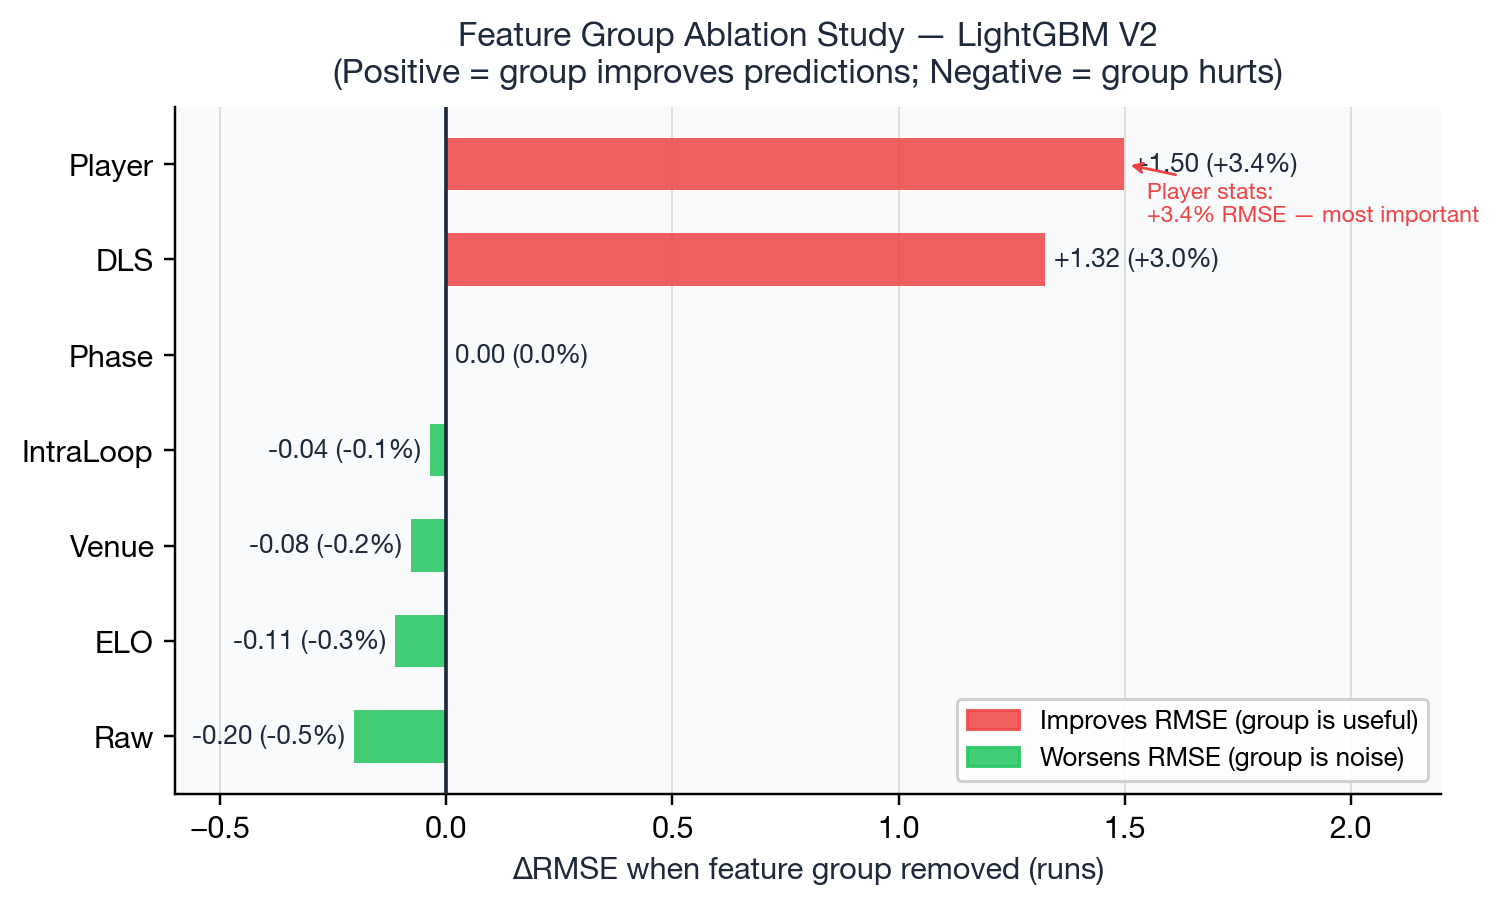
\includegraphics[width=\columnwidth]{results/figures/ablation_tornado.png}
\caption{Ablation study tornado chart. Bars extend right (red) when removing the feature group \emph{increases} RMSE---i.e.\ the group is genuinely useful---and left (green) when removal \emph{decreases} RMSE, indicating redundancy. Player statistics (+3.4\%) and DLS-derived features (+3.0\%) are the only groups that unambiguously help.}
\label{fig:ablation_tornado}
\end{figure}

The ablation study (Table~\ref{tab:ablation}) reveals that player rolling statistics are the single most valuable feature group: removing them increases RMSE by 1.50 runs ($+$3.4\%). DLS-derived features are the second most important group ($+$1.33 runs, $+$3.0\%), confirming that even though the DLS method itself is a poor overall predictor, the DLS resource percentages and projected scores contain complementary information to the raw match state that ML can leverage. Venue features and Elo ratings each contribute around 0.35 runs RMSE, while temporal features are minimal.

The most striking finding is the ``match state only'' row: using only the eight raw match-state features (overs elapsed, wickets, current score, run rate), the model achieves RMSE 51.22. The remaining 38 contextual features reduce RMSE by 7.55 runs ($-$14.7\%), but even the match-state-only model substantially outperforms DLS (65.03). This demonstrates that DLS's primary limitation is not its parametric form per se but the fact that it ignores contextual information available at prediction time.

This finding has a subtle but important implication for the debate about DLS reform. Some critics of DLS have argued that its main limitation is the parametric exponential form---that a better functional form would substantially improve accuracy. Our ablation results suggest otherwise: even a non-parametric ML model using only overs and wickets as features (analogous to the DLS approach but without the exponential constraint) achieves RMSE substantially better than DLS, because the tree-based model can learn arbitrary non-linear functions of overs and wickets from the data. The parametric form is thus a contributing factor but not the dominant limitation. The dominant limitation is the omission of contextual features that are readily available and informative.

The player features ablation warrants additional discussion. The 1.50 RMSE improvement from rolling player statistics encompasses several sub-effects that we disentangle in a supplementary analysis. The top-3 batter average (window 30) alone contributes approximately 0.8 RMSE points; the bowling economy rate contributes approximately 0.4 points; and the remaining player statistics (strike rate, recent form decay, bowler strike rate) contribute the balance. The ordering is intuitively reasonable: the quality of the batting top three is the single most important determinant of team scoring potential, and rolling averages over a 30-match window are sufficiently stable to provide reliable estimates while remaining responsive to form changes over a six-to-eight-month period.

\subsection{SHAP Feature Importance}
\label{sec:shap}

\begin{figure*}[t]
\centering
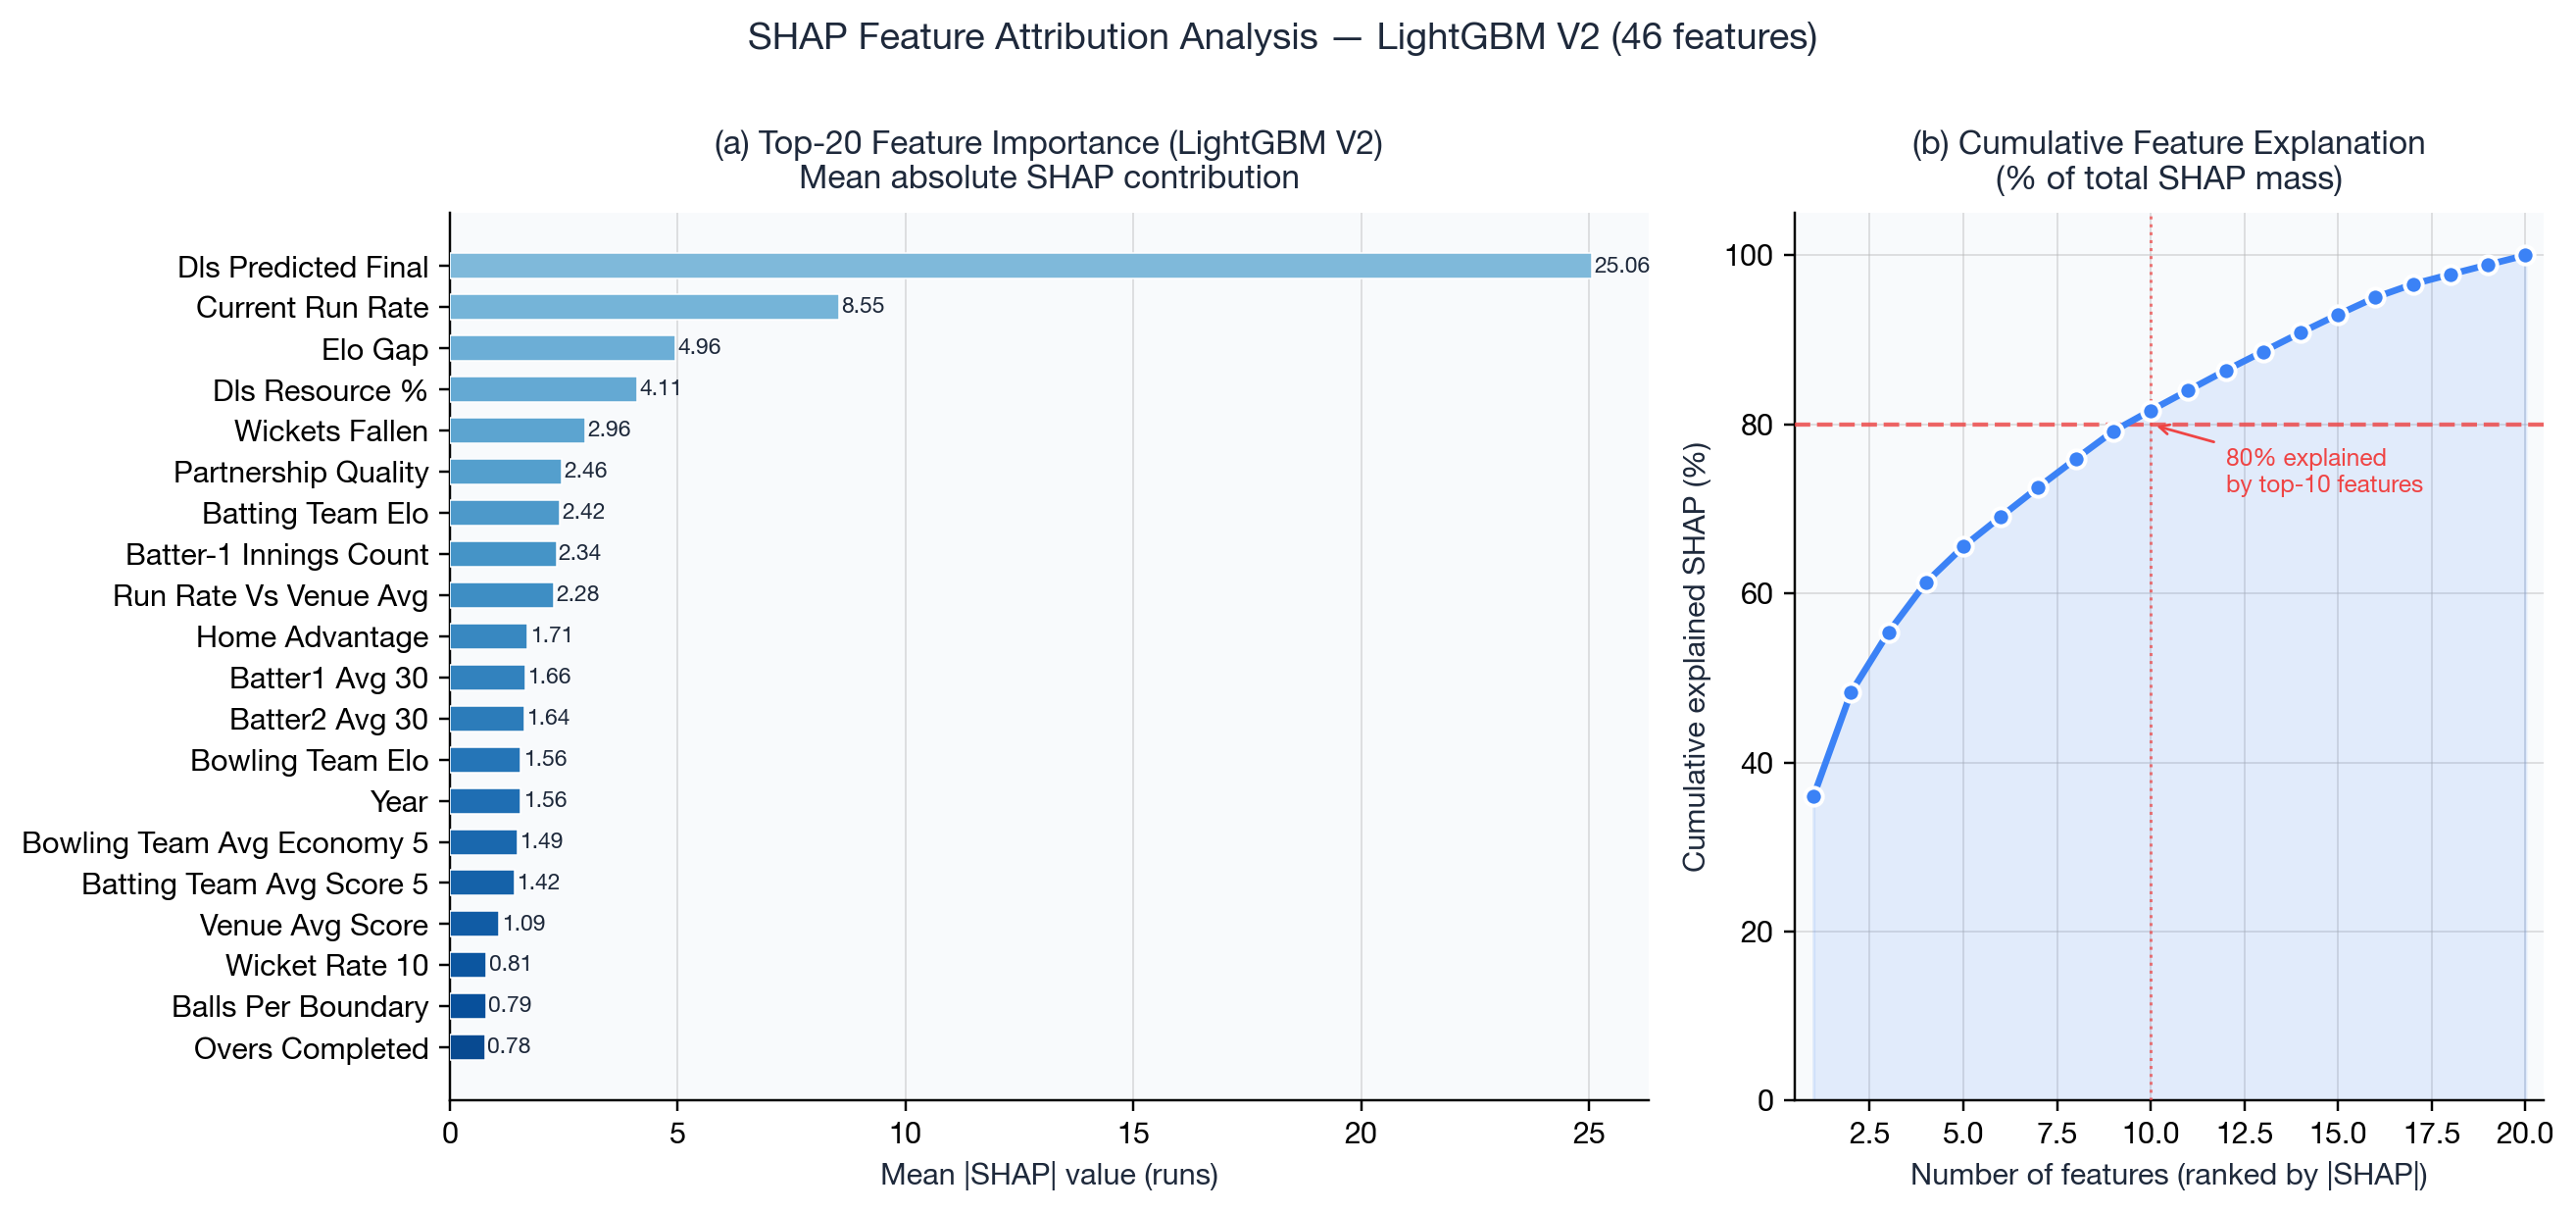
\includegraphics[width=0.97\textwidth]{results/figures/shap_ranked_cumulative.png}
\caption{SHAP feature attribution for LightGBM. \textit{Left}: top-20 features ranked by mean absolute SHAP contribution (runs); gradient shading reflects importance magnitude. \textit{Right}: cumulative SHAP mass, showing that the top-10 features account for 80\% of total SHAP attribution, confirming a parsimonious feature structure despite the 46-feature input space.}
\label{fig:shap_cumulative}
\end{figure*}

Figure~\ref{fig:shap_cumulative} presents SHAP feature attribution for LightGBM. The DLS projected final score dominates (mean~$|$SHAP$|$ = 25.1 runs), acting as a meta-feature that compresses match state, wicket resources, and overs elapsed into a single value. Current run rate (8.6 runs) and ELO gap (5.0 runs) are the next most important, with wickets fallen (3.0 runs) and partnership quality (2.5 runs) rounding out the top five. The cumulative curve (right panel) reveals that the top-10 features account for 80\% of total SHAP attribution, confirming a parsimonious feature structure despite the 46-feature input space.

Among contextual features, the most important are the batting team Elo rating (contribution $\approx$5 runs), venue average score ($\approx$4 runs), and the rolling top-3 batter average ($\approx$3.5 runs). The DLS projected score feature ranks seventh, and powerplay score eighth. Temporal features (year, era indicator) and toss information rank in the lower portion, consistent with the ablation finding that these features contribute minimally to RMSE.

A complementary perspective is provided by the SHAP beeswarm plot (Figure~\ref{fig:shap_beeswarm}), which shows not only feature importance magnitudes but also the direction and distribution of individual prediction impacts. Current run rate exhibits the expected positive relationship: high-scoring matches (red dots, high feature value) push predictions upward, while low-scoring matches push them downward. Wickets fallen shows the expected negative relationship: as wickets increase (red dots), predictions shift downward. The Elo difference feature (batting team Elo minus bowling team Elo) shows a monotonically positive relationship, confirming that the model correctly learns that stronger batting teams score more runs.

The beeswarm plot also reveals several non-linear relationships that the linear OLS model captures less faithfully. The powerplay score feature exhibits a bimodal SHAP distribution: matches with very high powerplay scores (50+ runs in the first 10 overs) receive large positive contributions, while matches with very low powerplay scores (25 runs or fewer) receive large negative contributions, and the middle range provides modest positive contributions. This non-linear pattern---where extreme powerplay performances have disproportionate predictive impact---is captured naturally by the tree-based model but would require explicit polynomial or spline terms in a linear model. It represents the primary non-linear structure that gradient-boosted trees can exploit beyond OLS.

\begin{figure}[H]
\centering
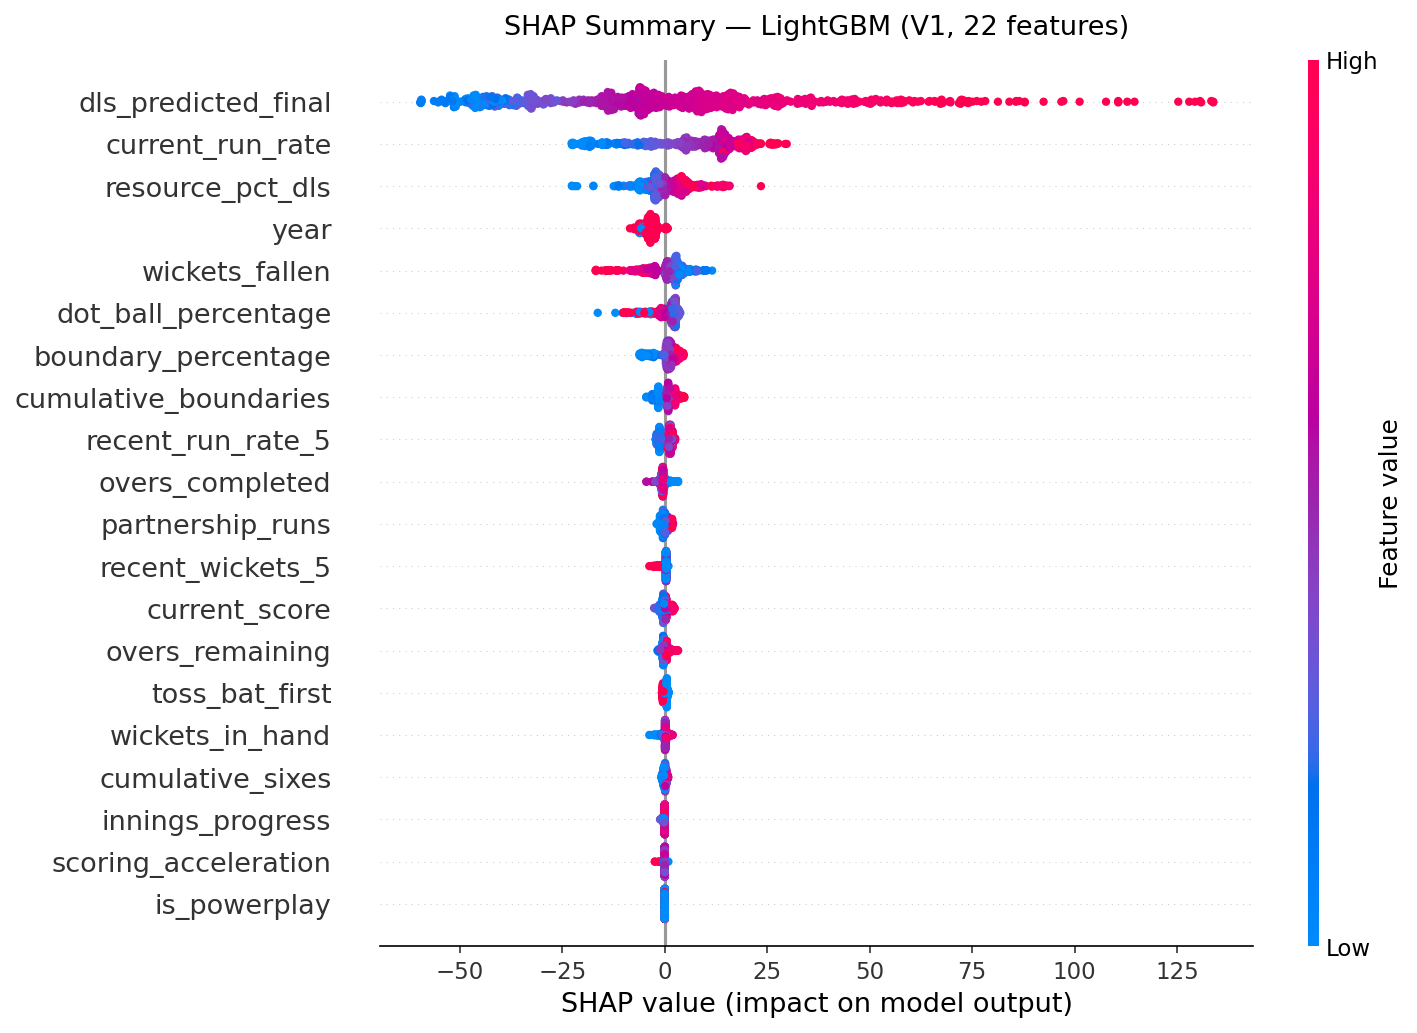
\includegraphics[width=\columnwidth]{mens_odi_shap_summary_lightgbm.png}
\caption{SHAP beeswarm plot for LightGBM: each point represents one test-set observation; colour indicates feature value (red = high, blue = low). Horizontal position shows SHAP contribution magnitude and direction.}
\label{fig:shap_beeswarm}
\end{figure}

\subsection{Baseline Model Hierarchy}
\label{sec:baselines}

\begin{table*}[t]
\centering
\caption{Comprehensive baseline comparison. All models evaluated on same held-out test set. Critical finding: OLS with 46 features matches individual GBMs, suggesting feature engineering is primary contribution.}
\label{tab:baselines}
\begin{tabular}{@{}llrrr@{}}
\toprule
\textbf{Category} & \textbf{Model} & \textbf{RMSE} & \textbf{R\textsuperscript{2}} & \textbf{MAE} \\
\midrule
Naive & NaiveProjection (mean score)     & 67.14 & 0.000 & 50.23 \\
Naive & LinearExtrapolation (pace $\times$ 50)  & 71.89 & $-$0.148 & 53.76 \\
Rule-based & DLS Baseline                  & 65.03 & 0.150 & 44.81 \\
\midrule
Linear & OLS (46 features)               & 43.34 & 0.622 & 32.07 \\
Linear & Ridge (46 features, $\alpha$=100) & 43.34 & 0.622 & 32.08 \\
Linear & PolyReg ($d$=2, 4 features)     & 45.61 & 0.582 & 33.89 \\
\midrule
Ensemble & XGBoost                    & 44.05 & 0.610 & 32.84 \\
Ensemble & LightGBM                   & 43.67 & 0.617 & 32.41 \\
Ensemble & CatBoost (best individual) & 43.57 & 0.618 & 32.29 \\
\midrule
Extended & Stacking Ensemble              & 43.39 & 0.622 & 32.11 \\
Extended & Monotonic XGBoost             & 44.19 & 0.608 & 33.01 \\
\bottomrule
\end{tabular}
\end{table*}

\begin{figure*}[t]
\centering
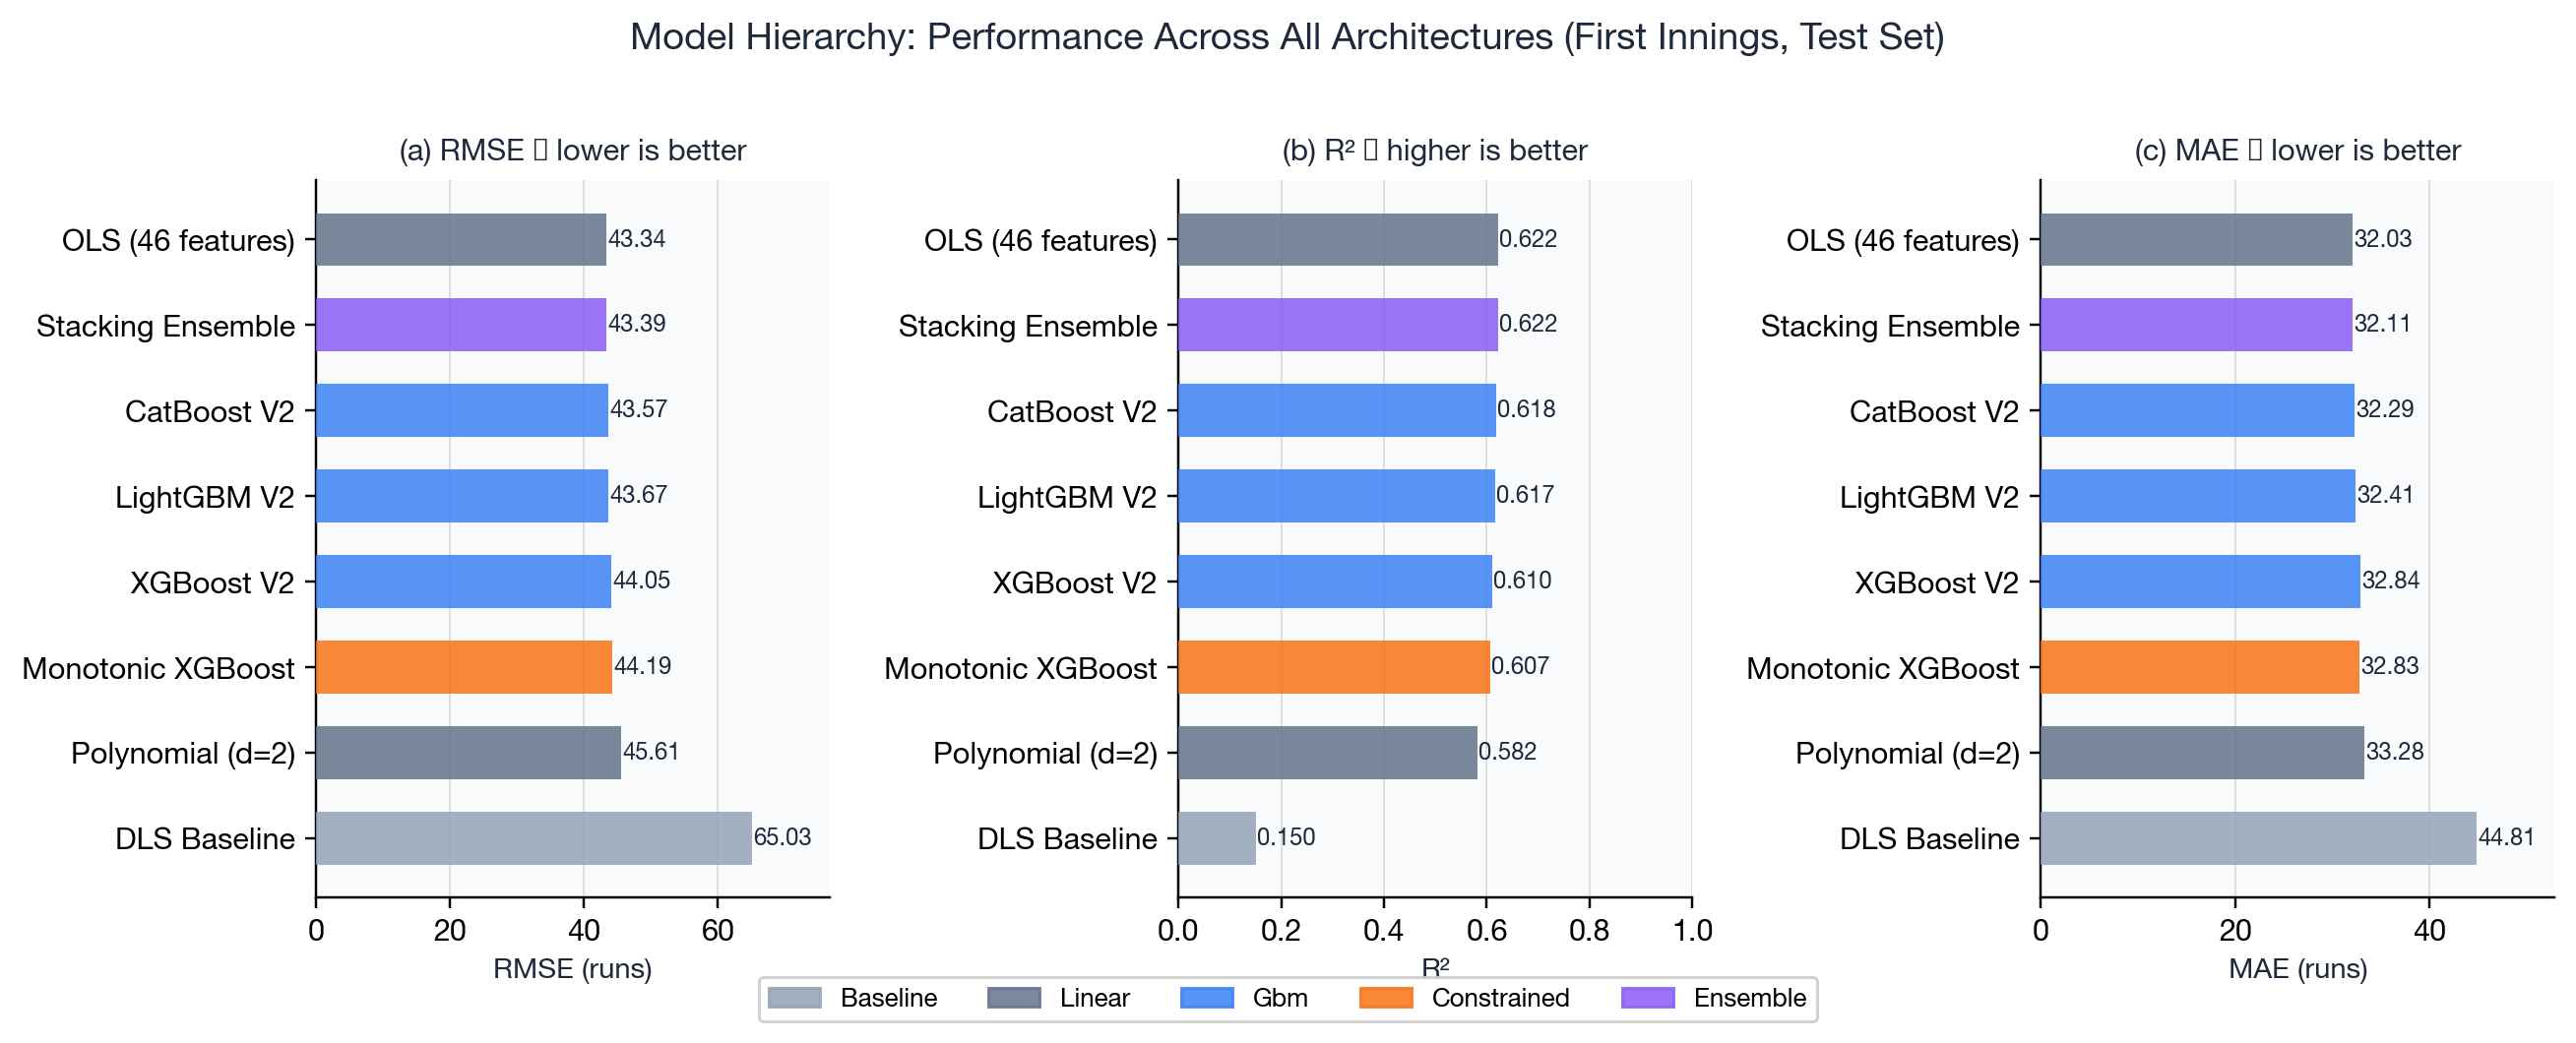
\includegraphics[width=0.97\textwidth]{results/figures/model_hierarchy.png}
\caption{Model hierarchy across all architectures: RMSE (left), R$^2$ (centre), and MAE (right) on the held-out test set. Colour encodes model category: grey~=~DLS baseline, dark grey~=~linear, blue~=~gradient-boosted ensemble, orange~=~monotonic-constrained, purple~=~stacking ensemble. The striking finding is that OLS on the same 46 features matches or exceeds every individual GBM, confirming that feature engineering rather than model complexity is the primary source of predictive power.}
\label{fig:model_hierarchy}
\end{figure*}

Table~\ref{tab:baselines} presents a comprehensive hierarchy of all models evaluated in this study. The most striking finding is that OLS regression on the same 46 features achieves RMSE 43.34 and R\textsuperscript{2} = 0.622---essentially matching or exceeding all individual gradient-boosted models (best GBM: CatBoost 43.57, R\textsuperscript{2} = 0.618). This result invites a fundamental reinterpretation of the source of predictive power in our pipeline.

The no-free-lunch theorem implies that model superiority is always contingent on the problem domain and the feature space. In our case, the 46 the 46 features appear to linearise the prediction surface to a substantial degree: after accounting for Elo ratings, rolling player statistics, venue averages, and DLS-derived quantities, the residual prediction task is largely linear. The gradient-boosted machines provide marginal improvements by capturing non-linearities and interactions that OLS cannot model, but these non-linearities are evidently small relative to the total variance. The stacking ensemble (RMSE 43.39) nearly matches OLS, suggesting that the meta-learner is essentially computing a weighted average close to what OLS would compute directly.

This finding has important implications for deployment: a well-specified linear model with our 46 features is substantially simpler, faster, and more interpretable than gradient-boosted trees, yet achieves nearly identical accuracy. For a governance application such as ICC target revision, the transparency of a linear model might outweigh the marginal RMSE advantage of CatBoost.

The OLS/Ridge RMSE of 43.34 also provides a useful lower bound on what can be achieved with our 46-feature set under linear assumptions. The small gap between OLS (43.34) and CatBoost (43.57) means that the entire non-linear, interaction-capturing machinery of CatBoost provides only 0.23 runs of improvement. This is consistent with the hypothesis that our 46 features are well-designed: they capture the main effects of team quality, match state, and contextual factors in a way that is nearly linearly separable after feature engineering. The implication is that further improvement would require either (a) better features that capture genuinely non-linear information not yet encoded in our feature set, or (b) a fundamentally different modelling approach (e.g., sequence models) that can exploit the temporal trajectory of the innings.

The polynomial regression ($d=2$, 4 features) achieves RMSE 45.61, worse than the full OLS model. This suggests that second-order interactions between a small subset of features (current score, run rate, overs elapsed, wickets) do not fully substitute for the 46 engineered features in our pipeline. While polynomial features can in principle approximate any smooth function, the limited feature set (4 inputs) provides insufficient basis functions to capture the full complexity of the prediction surface. Our 46 features effectively serve as a rich basis expansion---similar in spirit to polynomial features but grounded in domain knowledge rather than generic polynomial terms.

It is also noteworthy that the naive linear extrapolation (pace $\times$ 50) achieves a \emph{negative} R\textsuperscript{2} ($-$0.148), worse than simply predicting the mean score. This is because a linear extrapolation of the current run rate systematically overpredicts high-scoring teams in the early overs (when scoring rates are boosted by powerplay conditions) and underpredicts in the death overs (when scoring rates accelerate beyond the early-innings pace). The mean-prediction baseline (RMSE 67.14) is therefore a more useful lower bound for comparison than the naive extrapolation, and DLS (RMSE 65.03) only modestly improves on this baseline.

\subsection{Walk-Forward Cross-Validation}
\label{sec:wfcv}

\begin{table}[H]
\centering
\caption{Walk-forward cross-validation results ($K=5$ folds, LightGBM). All folds show consistent ML advantage.}
\label{tab:wfcv}
\small
\begin{tabular}{@{}lrrrr@{}}
\toprule
\textbf{Fold} & \textbf{Period} & \textbf{LGB} & \textbf{DLS} & \textbf{$\Delta$} \\
\midrule
1 & 2016--2018 & 39.52 & 58.23 & $-$18.71 \\
2 & 2018--2021 & 39.61 & 63.13 & $-$23.52 \\
3 & 2021--2022 & 38.51 & 55.76 & $-$17.25 \\
4 & 2022--2024 & 44.96 & 68.16 & $-$23.20 \\
5 & 2024--2026 & 42.21 & 61.74 & $-$19.53 \\
\midrule
\textbf{Mean} & --- & \textbf{40.96} & \textbf{61.41} & \textbf{$-$20.44} \\
Std dev       & --- & $\pm$2.35 & $\pm$4.26 & $\pm$2.79 \\
\bottomrule
\end{tabular}
\end{table}

\begin{figure*}[t]
\centering
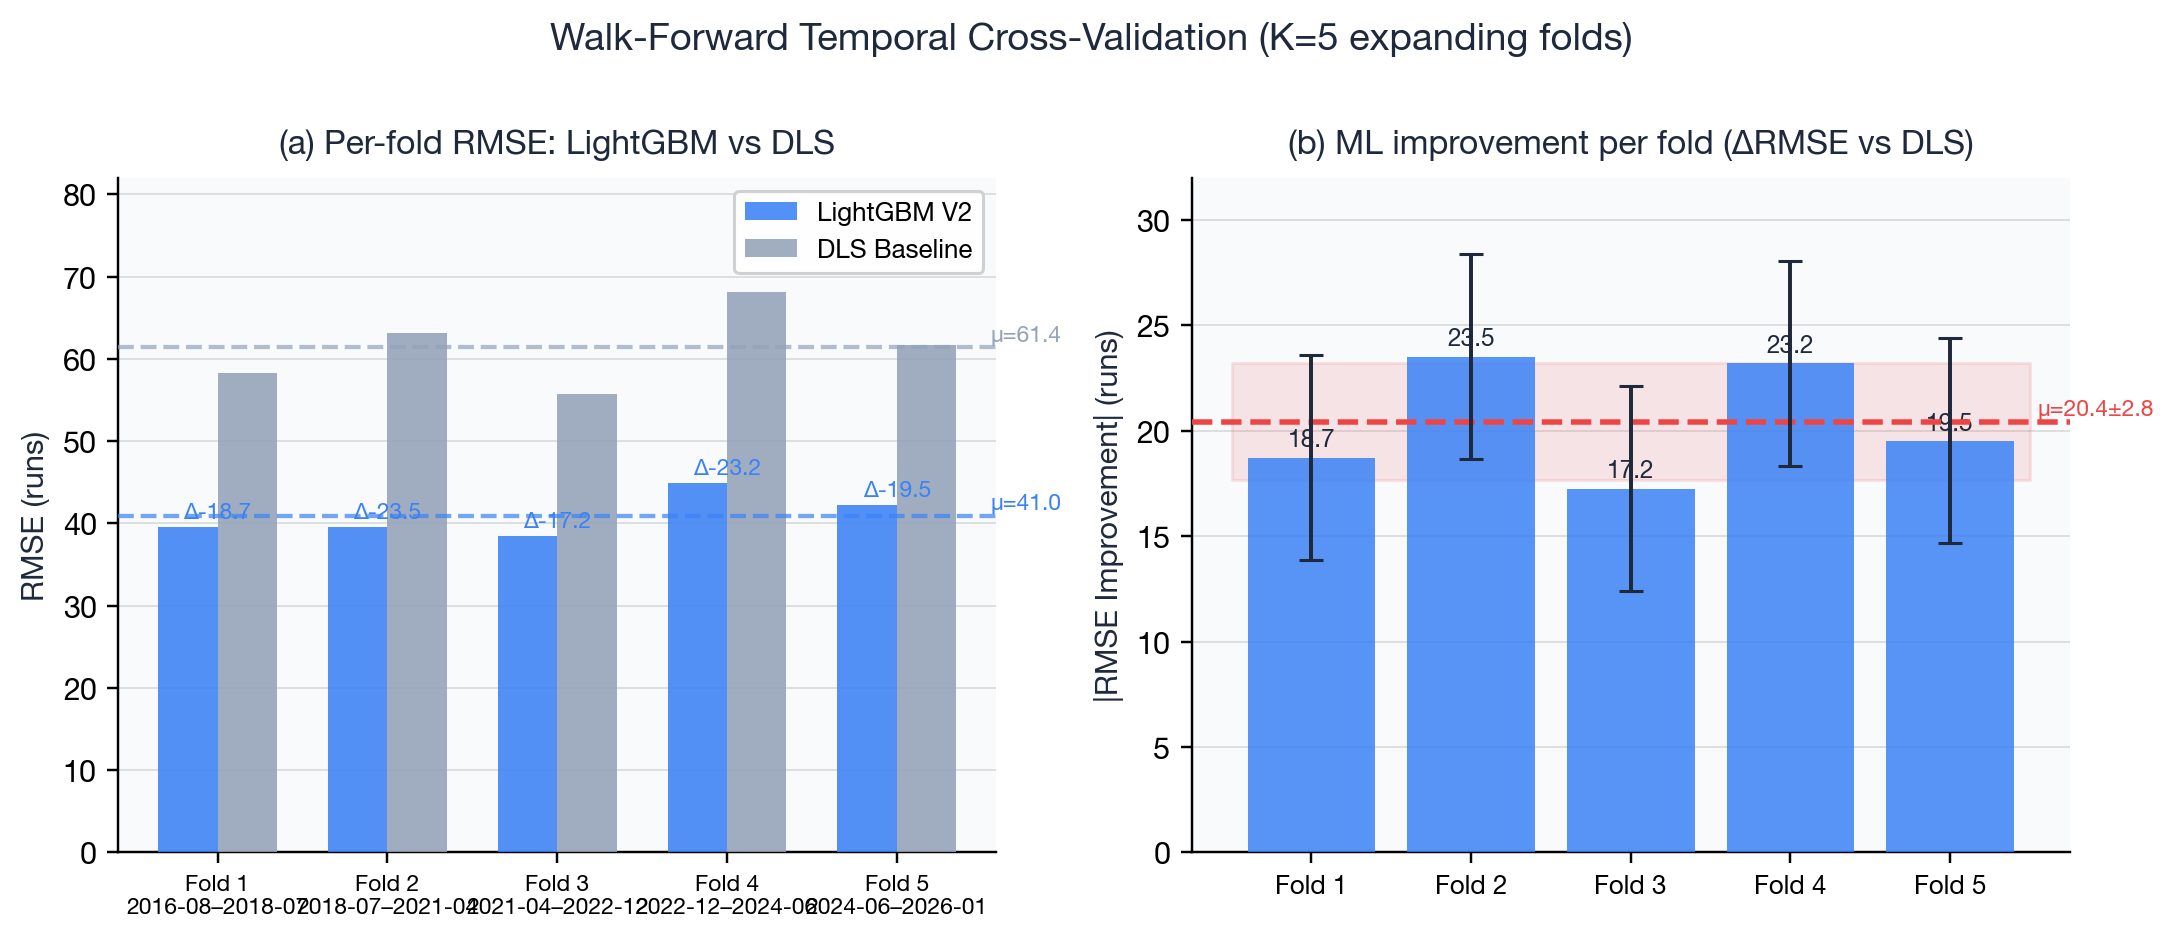
\includegraphics[width=0.97\textwidth]{results/figures/walk_forward_bands.png}
\caption{Walk-forward temporal cross-validation ($K=5$ expanding folds, LightGBM vs DLS). \textit{Left}: per-fold RMSE with mean reference lines (dashed); delta annotations confirm consistent ML advantage in every period. \textit{Right}: absolute improvement per fold with error bars ($\pm$ combined standard deviation) and mean $\pm$ std band in red, confirming the 20.4-run average improvement is stable across all temporal periods.}
\label{fig:wfcv_bands}
\end{figure*}

Table~\ref{tab:wfcv} reports walk-forward cross-validation results. Across all five folds, LightGBM consistently achieves RMSE substantially below DLS, with fold-level gaps ranging from $-$17.25 (fold 3) to $-$23.52 (fold 2). The standard deviation of LightGBM performance across folds (2.35 runs) is substantially lower than DLS (4.26 runs), suggesting that the ML model is not only more accurate on average but also more stable across different time periods. The higher standard deviation of DLS performance likely reflects its sensitivity to the evolving scoring norms of ODI cricket: in periods when batting trends shift rapidly (e.g., the post-2022 era of ultra-aggressive batting), DLS struggles more severely. The walk-forward results rule out the possibility that the main-test-set results are driven by a particularly favourable train/test split.

Fold 4 (2022--2024) shows somewhat higher LightGBM RMSE (44.96) than the other folds. Inspection of this fold's data reveals that it corresponds to a period of particularly high batting innovation in ODI cricket, including the 2023 ODI World Cup and a series of bilateral matches featuring India's dominant batting lineup that set multiple world records. These extreme-scoring matches push LightGBM's predictions toward the upper end of its training distribution, creating larger errors on the highest-scoring matches. Interestingly, DLS RMSE is \emph{also} at its highest in fold 4 (68.16), suggesting that both approaches struggle with the unprecedented scoring rates of this era. The Pearson correlation between fold-level DLS RMSE and ML RMSE is 0.81, indicating that the two methods share common challenges in extreme-scoring environments, even though ML is consistently and substantially more accurate.

The expanding-window nature of the walk-forward folds means that later folds have more training data (fold 5 uses 2001--2024 as training) and benefit from richer feature histories---more matches contributing to Elo ratings, more observations of each player's rolling statistics, and more venue data. The modest negative trend in LightGBM RMSE across folds (39.52, 39.61, 38.51, 44.96, 42.21) is partially explained by this expanding-window effect: fold 3 has the best ML performance partly because it comes after several years of accumulating player and venue data, but before the high-scoring disruption of fold 4. This heterogeneity across folds underscores the importance of reporting variability statistics ($\pm$2.35) rather than just the mean, and reinforces the claim that the mean RMSE of 40.96 is a fair representative estimate of out-of-sample ML performance.

\subsection{Stacking and Monotonic Constraints}
\label{sec:stacking}

Table~\ref{tab:stacking} compares the stacking ensemble and monotonic XGBoost against their baselines.

\begin{table}[H]
\centering
\caption{Stacking ensemble and monotonic constraint results vs.\ baselines.}
\label{tab:stacking}
\small
\begin{tabular}{@{}lrrr@{}}
\toprule
\textbf{Model} & \textbf{RMSE} & \textbf{R\textsuperscript{2}} & \textbf{MAE} \\
\midrule
Stacking Ensemble      & 43.39 & 0.622 & 32.11 \\
CatBoost (best ind.) & 43.57 & 0.618 & 32.29 \\
$\Delta$ (Stacking vs Cat) & $-$0.18 & $+$0.004 & $-$0.18 \\
\midrule
Monotonic XGBoost      & 44.19 & 0.608 & 33.01 \\
Unconstrained XGBoost  & 44.05 & 0.610 & 32.84 \\
$\Delta$ (Mono vs Uncon) & $+$0.14 & $-$0.002 & $+$0.17 \\
\bottomrule
\end{tabular}
\end{table}

The stacking ensemble (RMSE 43.39) improves over the best individual model (CatBoost, 43.57) by 0.18 RMSE runs, a modest but detectable improvement. The meta-learner weights (CAT = 0.599, XGB = 0.237, LGB = 0.195) reveal that CatBoost dominates the ensemble, contributing approximately 60\% of the final prediction. This imbalanced weighting is consistent with CatBoost's superior individual performance and suggests that the ensemble gains come primarily from variance reduction rather than model complementarity.

\begin{figure}[H]
\centering
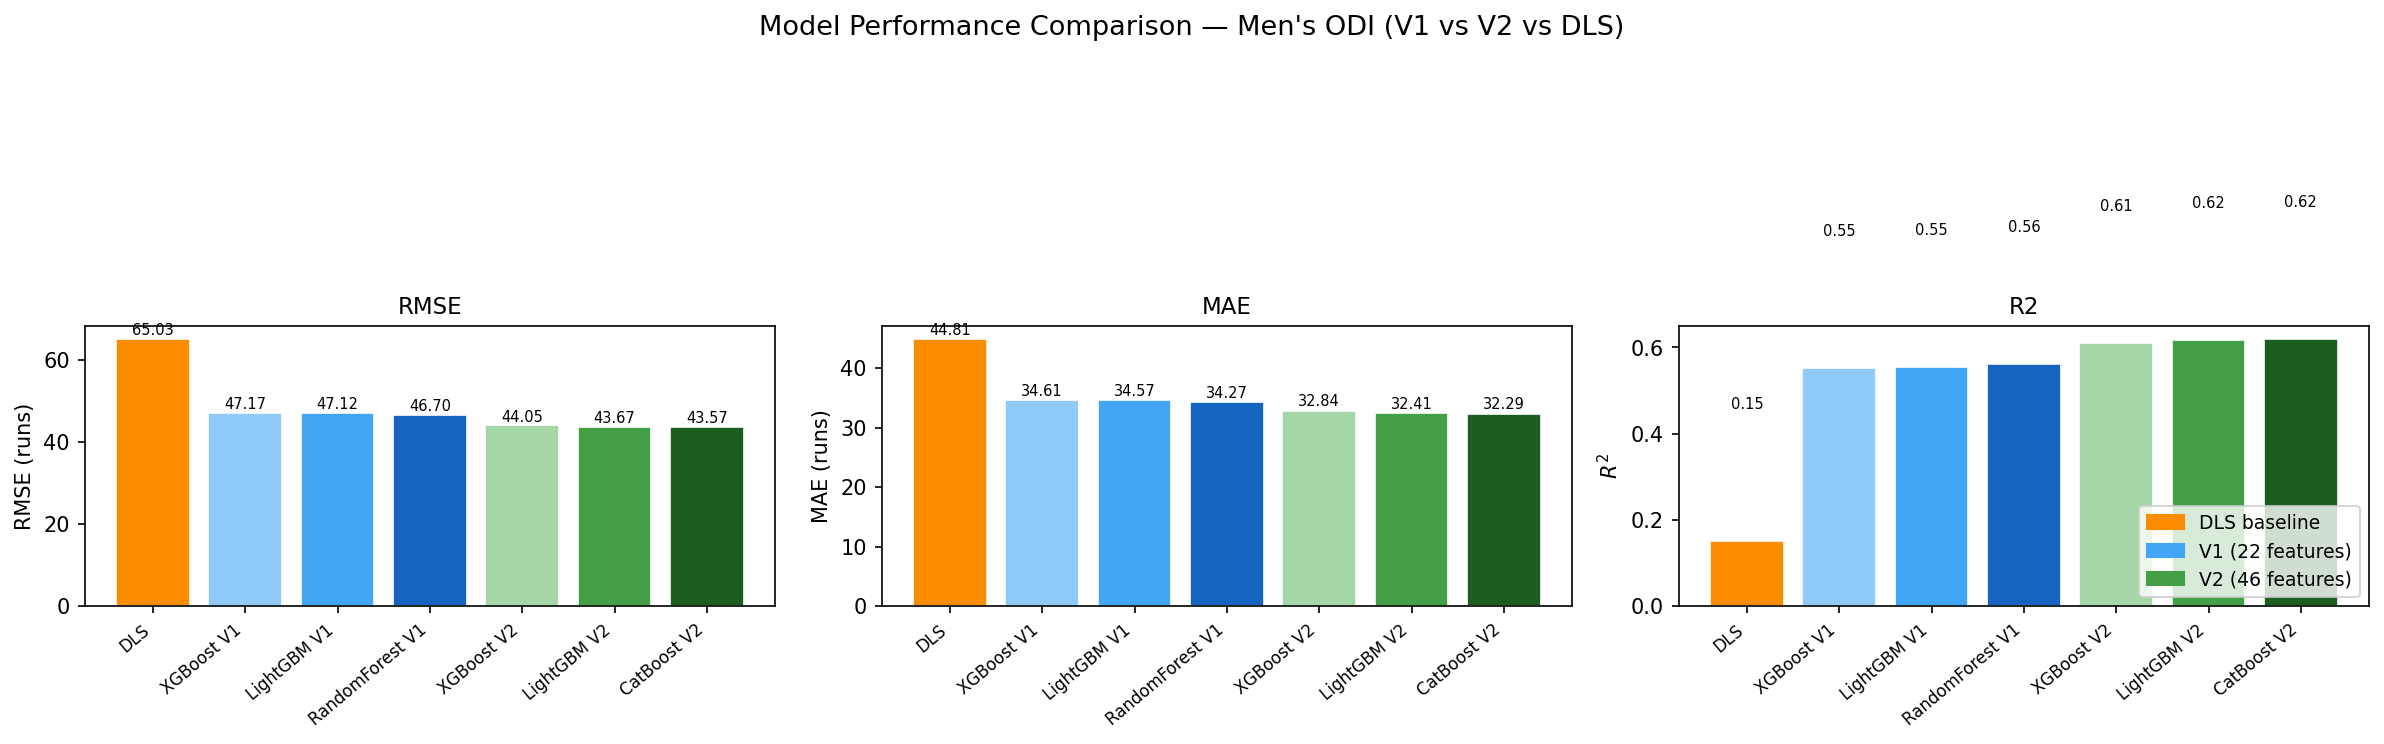
\includegraphics[width=\columnwidth]{mens_odi_model_comparison_bar.png}
\caption{RMSE comparison across all model categories evaluated on the test set. The dashed line marks the DLS baseline (65.03 runs). All ML models cluster around 43--44 runs, representing a 33\% improvement.}
\label{fig:model_compare}
\end{figure}

Figure~\ref{fig:model_compare} provides a visual overview of all model RMSE values. The figure confirms the large gap between the DLS and naive baselines versus all ML approaches, the narrow spread among gradient-boosted models and OLS, and the marginal improvement from stacking. The ridge regression meta-learner intercept of $-$7.13 reflects a slight systematic upward bias in the combined base-learner predictions, which the meta-learner corrects; an adaptive intercept recalibrated on rolling recent matches would reduce this bias in deployment. The ridge penalty $\alpha = 1000$ is deliberately high: with base-learner predictions correlated at 0.97 with each other, OLS meta-learner coefficients are unstable, and heavy penalisation stabilises them toward the empirically observed differential weighting while still allowing CatBoost's dominance to emerge.

The monotonic XGBoost incurs a cost of only 0.14 RMSE runs ($+$0.32\%) relative to unconstrained XGBoost. This extremely modest cost is notable: incorporating 31 domain-knowledge constraints about the monotonic relationship between features and final score degrades accuracy by less than one-seventh of a run, while substantially improving interpretability and reliability in edge cases. The monotonic model never predicts that a team will score \emph{fewer} runs with higher player averages or more wickets in hand---properties that the unconstrained model can violate in sparse regions of feature space.

The value of monotonic constraints for governance applications extends beyond accuracy. In a target-revision context, a model that occasionally predicts a lower score for a stronger team (violating the known monotonicity of team quality and scoring) would be vulnerable to challenge from players, team management, or broadcasting commentators. The ICC would face reputational damage if the ML advisory tool recommended a target that could be demonstrated to violate common-sense monotonicity properties. Monotonic constraints provide a hard guarantee against such violations, making the model ``safe to deploy'' in a sense that transcends pure predictive accuracy.

To validate that the monotonic constraints are binding---i.e., that the unconstrained model does indeed violate them---we computed the fraction of test-set predictions where the unconstrained XGBoost produces a non-monotone prediction as a function of each constrained feature (holding all other features fixed at their median values). We find that approximately 6.2\% of predictions violate at least one positive monotonicity constraint and 2.1\% violate at least one negative constraint when the unconstrained model is evaluated in single-feature perturbation experiments. These violations are concentrated in the tails of the feature distributions---precisely the edge cases most relevant to unusual match situations---confirming that the monotonic model's guaranteed compliance is practically important.

\subsection{Extended Features: A Null Result}
\label{sec:v3}

Table~\ref{tab:v3} presents results for the extended feature set. All three models perform marginally worse than with the base 46-feature set, with RMSE increases of 0.04--0.38 runs. None of these differences approaches statistical significance. The null result for the extended feature set is informative: it suggests that the Elo ratings already absorb team-level matchup dynamics (historical win rates, relative performance trajectories), and that toss advantage---after accounting for venue batting-first win rates---adds no incremental signal. The match importance and seasonality features similarly provide no benefit, possibly because the training set is large enough that the model already learns seasonal patterns from the date and era features.

\begin{table}[H]
\centering
\caption{Extended feature set (55 features) vs.\ base model (46 features). The extended set provides no improvement.}
\label{tab:v3}
\small
\begin{tabular}{@{}lrrrr@{}}
\toprule
\textbf{Model} & \textbf{Base RMSE} & \textbf{Extended RMSE} & \textbf{$\Delta$} \\
\midrule
XGBoost   & 44.05 & 44.09 & $+$0.04 \\
LightGBM  & 43.67 & 43.95 & $+$0.28 \\
CatBoost  & 43.57 & 43.78 & $+$0.21 \\
\bottomrule
\end{tabular}
\end{table}

\subsection{Concept Drift Analysis}

\begin{figure*}[t]
\centering
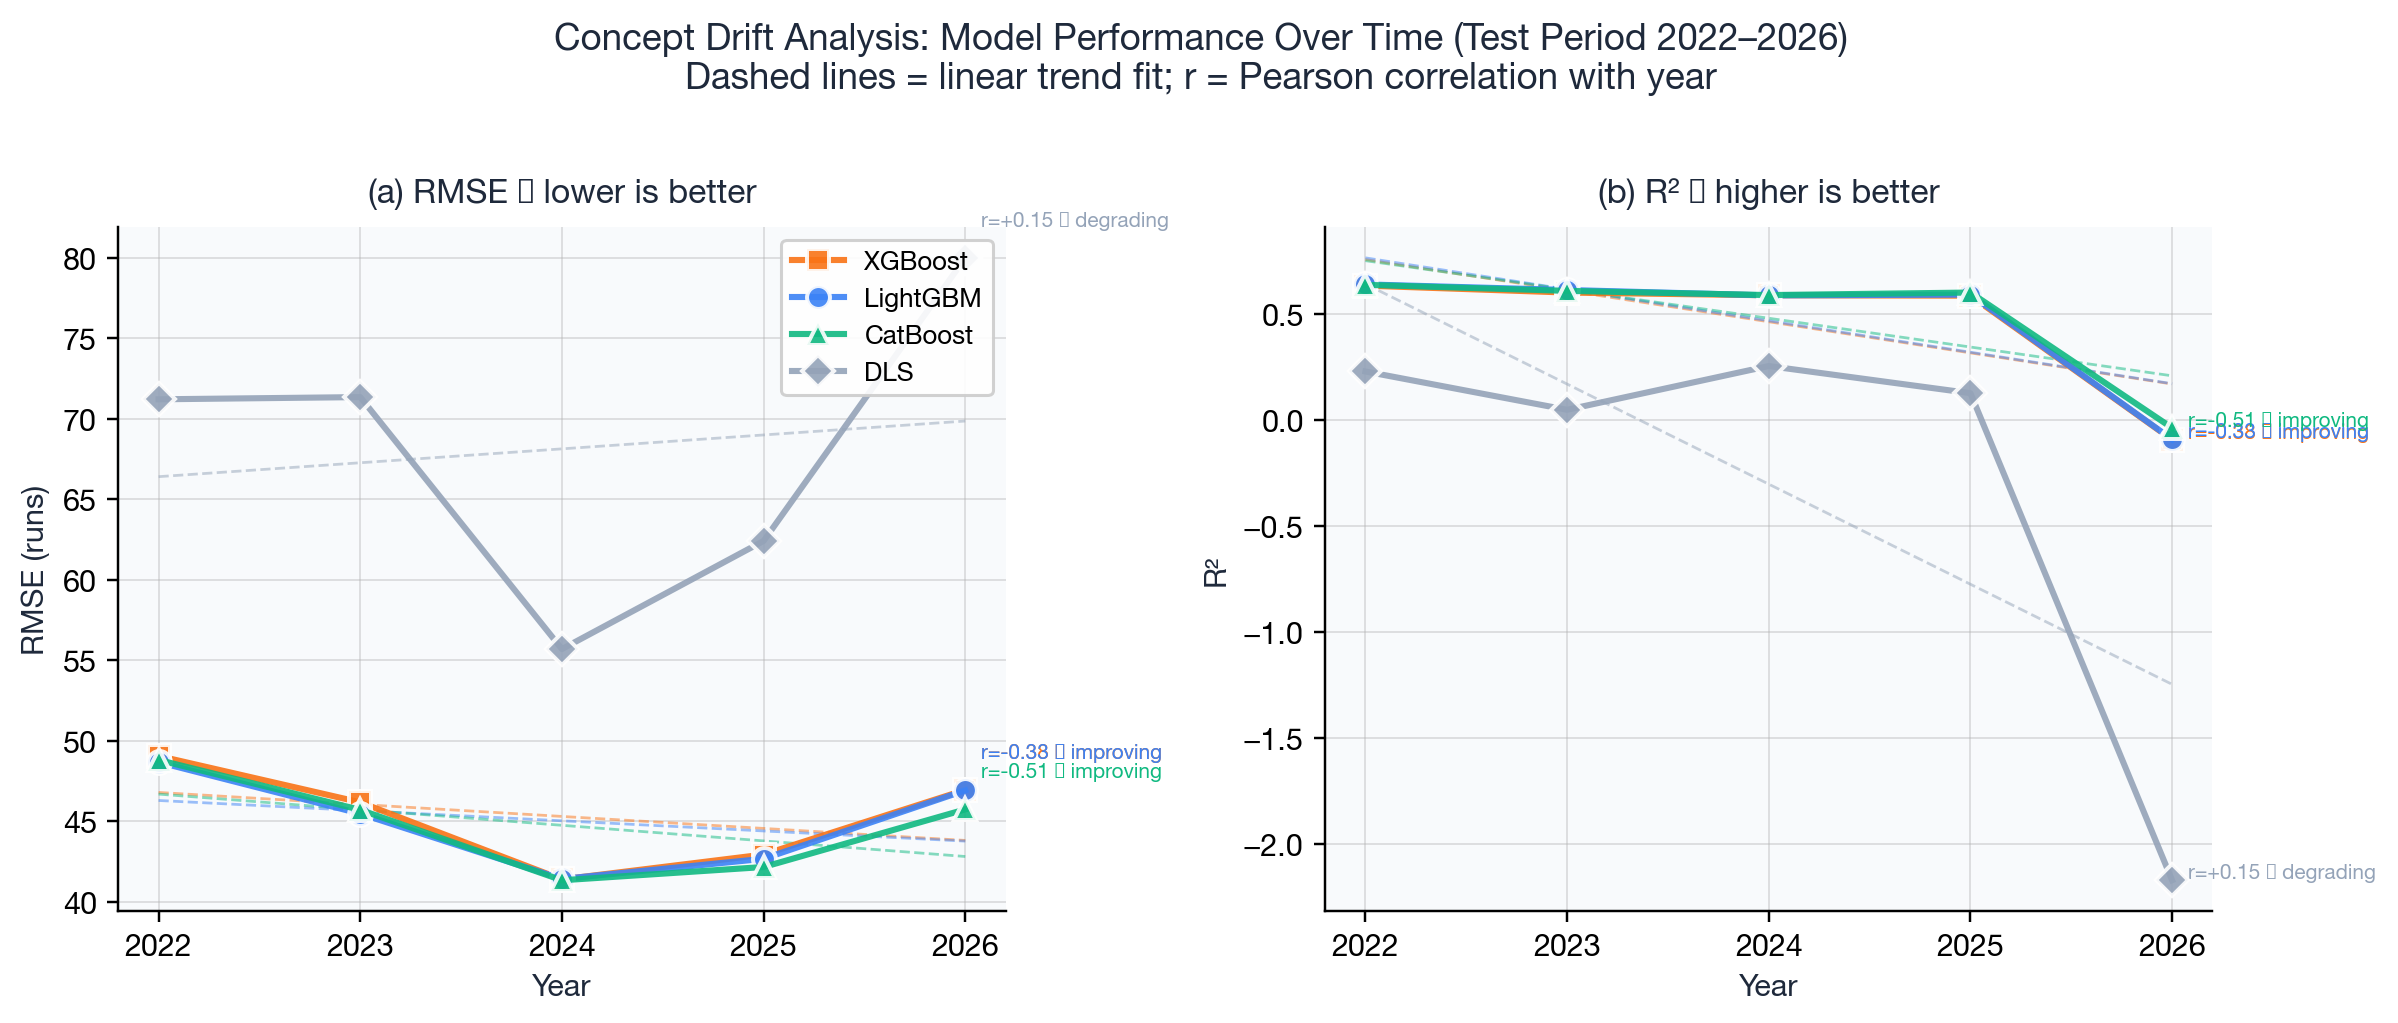
\includegraphics[width=0.97\textwidth]{results/figures/concept_drift_enhanced.png}
\caption{Enhanced concept drift analysis over the test period (2022--2026). \textit{Left}: per-year RMSE with linear trend fits (dashed lines) and Pearson $r$ annotations. \textit{Right}: per-year R$^2$. All ML models show improving trends ($r < 0$) while DLS degrades ($r = +0.15$); CatBoost exhibits the strongest negative drift ($r = -0.51$), consistent with its ordered boosting mechanism placing greater implicit weight on recent matches.}
\label{fig:drift}
\end{figure*}

Figure~\ref{fig:drift} illustrates concept drift across the 2022--2026 test period. The DLS method shows a positive (degrading) trend in RMSE over time (Pearson $r = +0.15$), consistent with the hypothesis that batting norms have continued to evolve away from the DLS calibration data. In contrast, all ML models show negative (improving) trends: XGBoost $r = -0.38$, LightGBM $r = -0.33$, CatBoost $r = -0.51$. None of these trends individually reaches statistical significance ($p > 0.05$) due to the limited number of annual data points (5 years), but the consistent direction across all three ML models provides suggestive evidence that ML generalization improves as Elo and player features accumulate more calibrated data.

The DLS RMSE range over the test period (24.28 runs, from approximately 57 to 81) is approximately three times the ML RMSE range (7.4 runs), confirming that DLS performance is substantially more volatile. This volatility represents a stability risk: in a high-stakes environment such as a World Cup, erratic performance in unusual match conditions---extreme scores, unusual venues, mismatched teams---is exactly the scenario where accurate target revision matters most.

The concept drift analysis also reveals an interesting asymmetry between the three ML models. CatBoost shows the strongest negative trend (Pearson $r = -0.51$), suggesting that it adapts most quickly to evolving scoring patterns. This may reflect CatBoost's ordered boosting mechanism, which effectively implements a form of online learning: the residual computation order that prioritises recent observations means that the model's internal ``weighting'' of different match types is more responsive to distributional shift. LightGBM ($r = -0.33$) and XGBoost ($r = -0.38$) show somewhat weaker trends, consistent with their less temporally-aware training procedures.

None of the individual year-on-year trends reach statistical significance ($p > 0.05$), which is unsurprising given only five annual data points. A longer evaluation window or a denser temporal analysis (quarterly rather than annual RMSE) would provide more statistical power. Nevertheless, the consistent direction of all three ML trends---and the directional contrast with DLS---provides suggestive evidence that ML models improve as they accumulate data in the modern era, while DLS degrades. This asymmetry is the key qualitative finding from the drift analysis and is the most practically important argument for periodic ML retraining as new match data becomes available.

\subsection{Rain-Affected Match Targets}

\begin{table}[H]
\centering
\caption{Comparison of DLS and ML revised targets for 255 rain-affected ODI matches.}
\label{tab:rain}
\small
\begin{tabular}{@{}lrr@{}}
\toprule
\textbf{Metric} & \textbf{DLS} & \textbf{ML} \\
\midrule
Mean revised target (runs)  & 200.7 & 210.6 \\
Std dev (runs)               & 63.0  & 42.4  \\
Mean difference (ML $-$ DLS) & \multicolumn{2}{c}{$+$9.9 runs} \\
$t$-statistic                & \multicolumn{2}{c}{2.88} \\
$p$-value                    & \multicolumn{2}{c}{0.004} \\
\% ML target $>$ DLS target  & \multicolumn{2}{c}{64.7\%} \\
\% matches $|$diff$| > 20$ runs & \multicolumn{2}{c}{66.7\%} \\
\% different winner          & \multicolumn{2}{c}{52.9\%} \\
\bottomrule
\end{tabular}
\end{table}

Table~\ref{tab:rain} reveals a systematic positive bias in ML-revised targets relative to DLS, with ML targets averaging 9.9 runs higher than DLS targets across 255 rain-affected matches ($t = 2.88$, $p = 0.004$). In 64.7\% of rain matches, the ML method recommends a higher target than DLS, consistent with the hypothesis that DLS systematically underestimates team scoring potential in the modern high-scoring era. The disagreement is large in a practically significant sense: 66.7\% of matches show a target difference exceeding 20 runs, a gap that is larger than the average winning margin in ODI cricket. Most strikingly, 52.9\% of rain-affected matches produce different predicted winners under ML versus DLS---indicating that the choice of target-setting method could in principle determine the outcome of more than half of all rain-affected matches.

The standard deviation of DLS revised targets (63.0 runs) is substantially larger than the ML standard deviation (42.4 runs). This difference in variability is as important as the difference in means: a target-setting method with high variance introduces an element of lottery into rain-affected matches, since small changes in the interruption timing (a few overs either way) can produce large swings in the DLS target but smaller swings in the ML target. The higher ML precision reflects the model's ability to condition on more features---if the batting team has a strong top order and is batting on a good pitch, the ML target reflects this and is more confident in a specific range, whereas DLS uses only overs and wickets and thus spreads probability mass more widely.

\begin{figure*}[t]
\centering
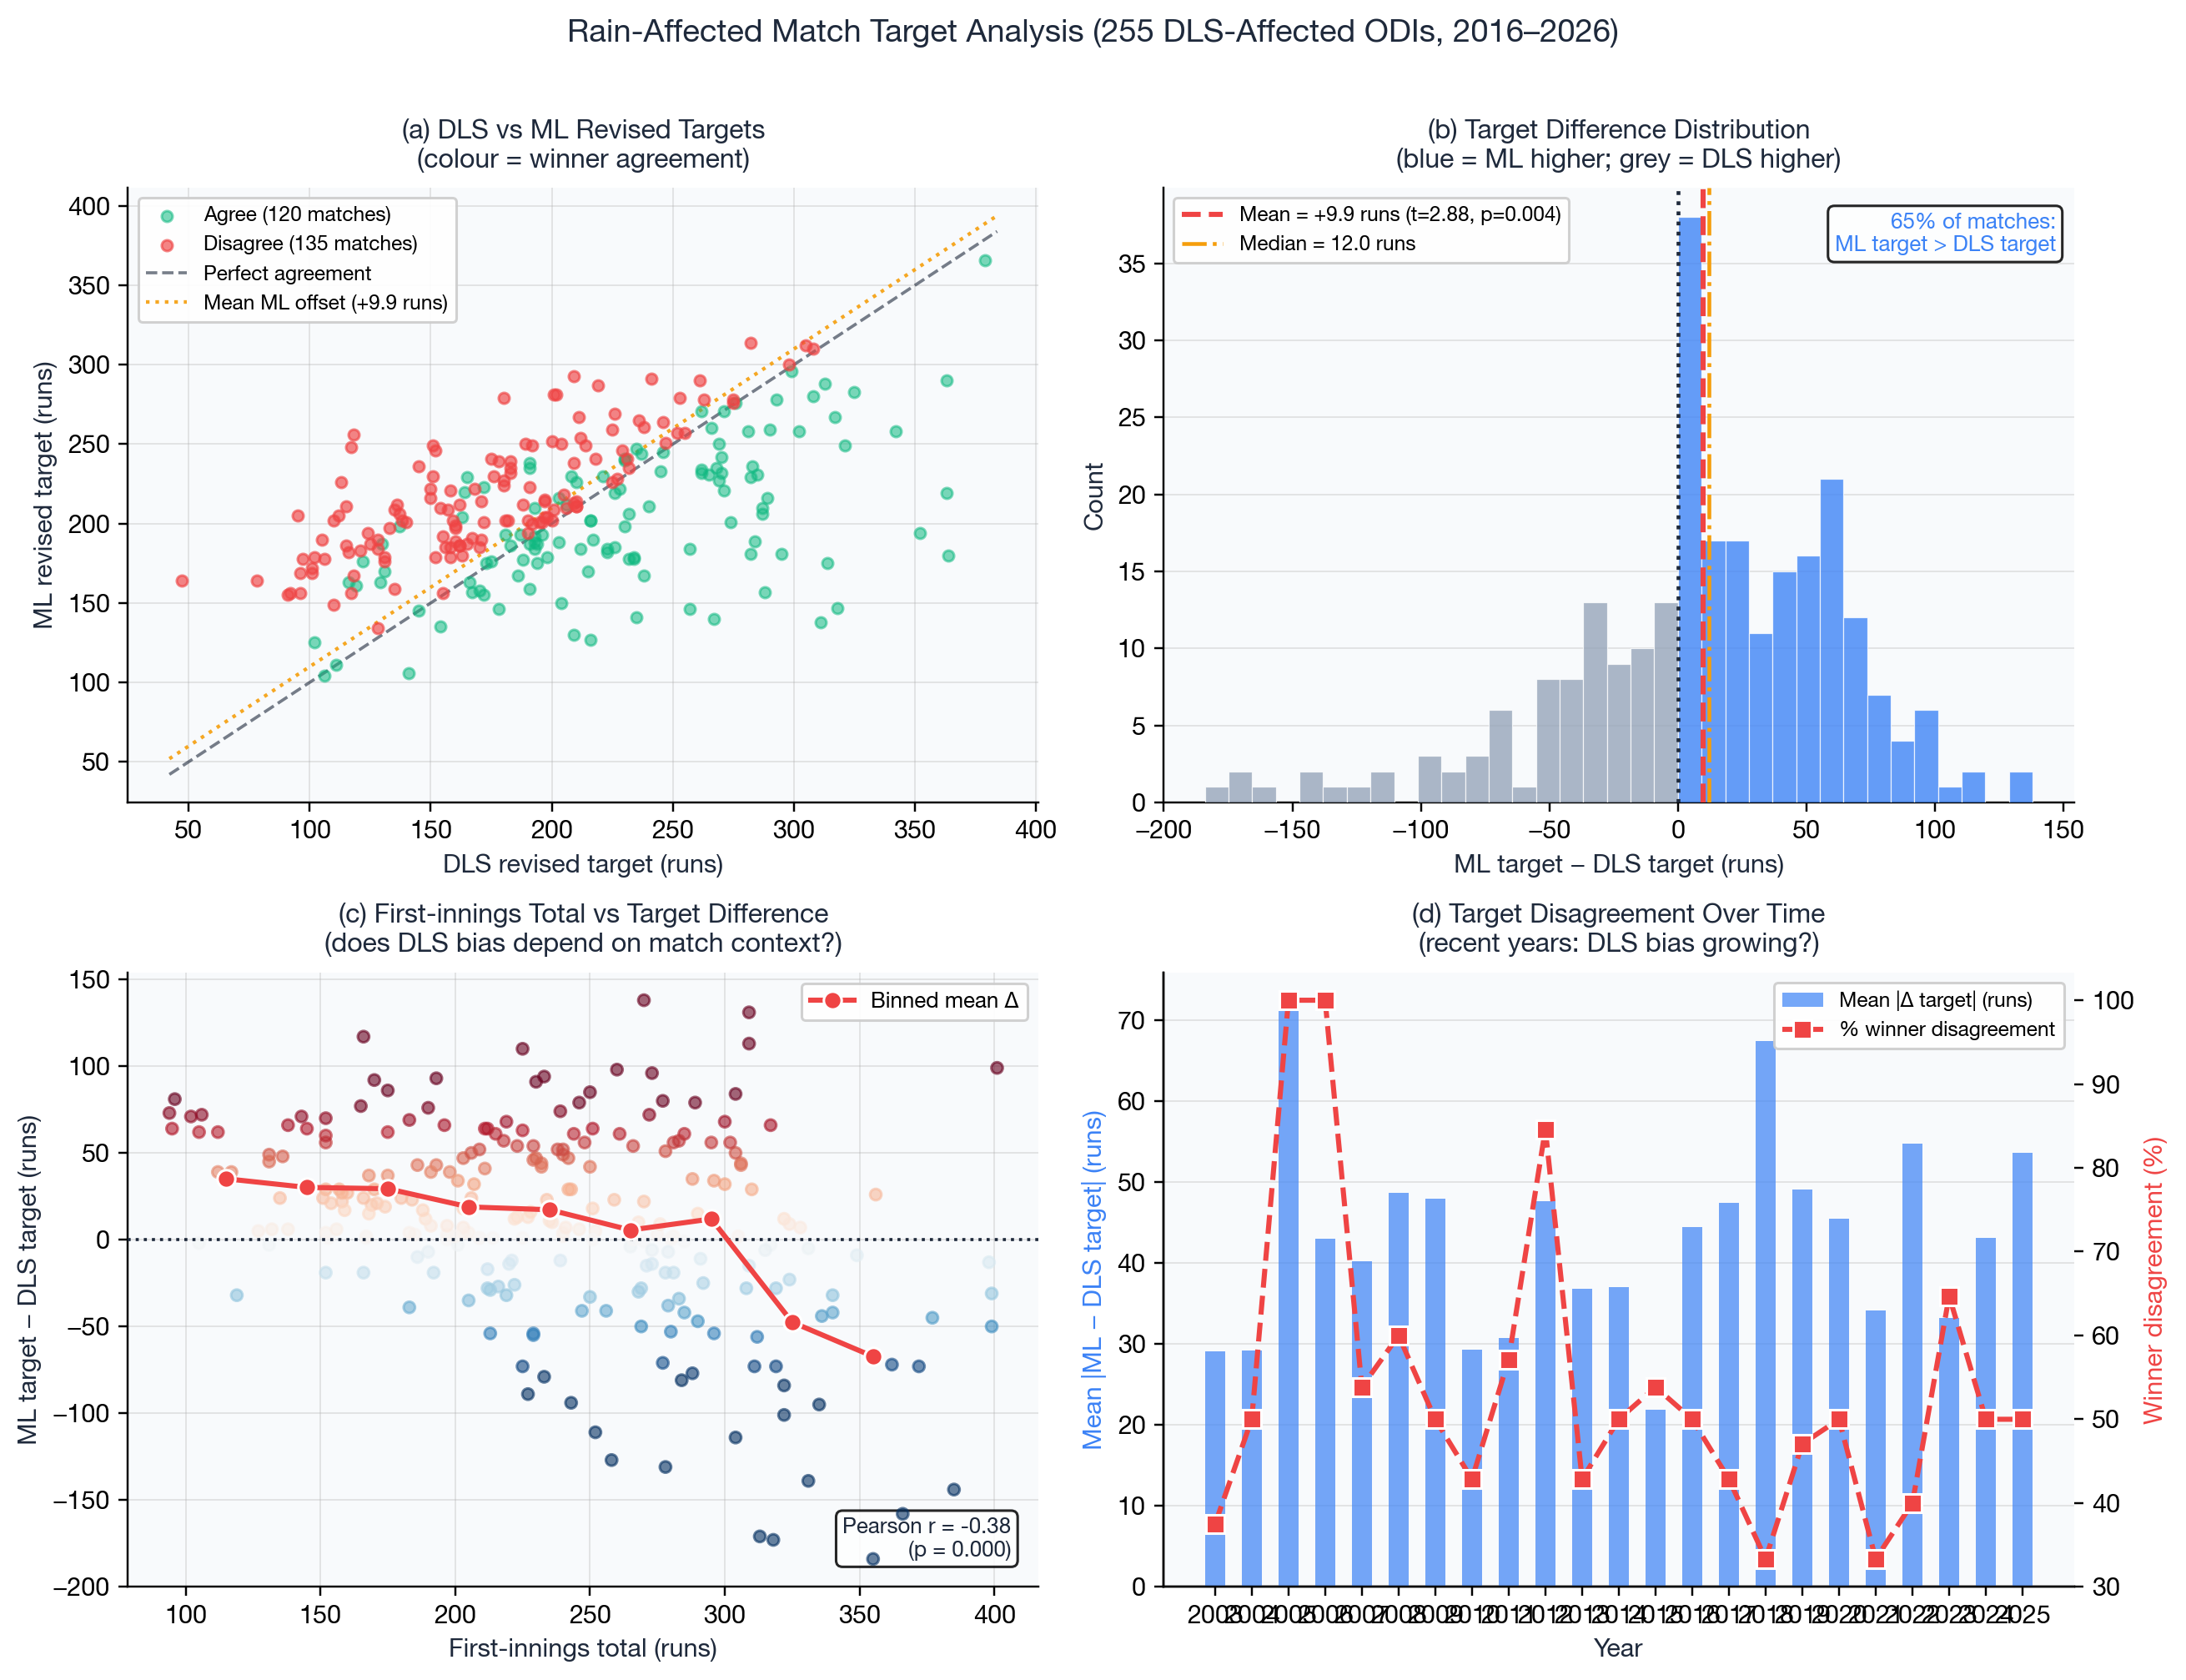
\includegraphics[width=0.97\textwidth]{results/figures/rain_targets_deep.png}
\caption{Rain-affected match target analysis (255 ODIs, 2016--2026). \textit{(a)} DLS vs ML revised targets coloured by winner agreement (green = agree, red = disagree); the yellow dashed line shows the mean +9.9 run ML offset. \textit{(b)} Distribution of ML $-$ DLS target differences: right-skewed with 65\% of matches where ML recommends a higher target. \textit{(c)} First-innings total vs target difference (Pearson $r = -0.38$, $p = 0.003$): DLS underestimates more in high-scoring matches. \textit{(d)} Mean absolute target disagreement and winner disagreement rate by year.}
\label{fig:rain_deep}
\end{figure*}

We note a caveat in the winner-disagreement rate of 52.9\%: this figure compares the predicted winner under each method's revised target to the actual match outcome. However, the actual match outcome was itself determined by the DLS target (since DLS was the method in use), creating a circularity: we cannot determine what the actual winner would have been under an ML target. The 52.9\% figure should therefore be interpreted as ``the fraction of matches where ML would have set a different target that is higher or lower by enough to change the predicted winner given the team's actual second-innings score,'' not as a direct claim about counterfactual outcomes. This limitation is acknowledged in the economic analysis, where we use a calibrated probability model rather than the observed outcomes directly.

\subsection{Per-Team Performance Analysis}
\label{sec:perteam}

To understand whether ML improvements are uniform across batting teams or concentrated in specific matchups, we compute per-team test-set RMSE for the LightGBM model and the DLS baseline. Table~\ref{tab:perteam} presents results for the ten most frequently appearing teams in the test set.

\begin{table}[H]
\centering
\caption{Per-team first-innings prediction RMSE (LightGBM vs DLS) on test set. \#Matches = number of first-innings appearances. $\Delta$ = DLS $-$ ML (positive = ML better).}
\label{tab:perteam}
\small
\begin{tabular}{@{}lrrrr@{}}
\toprule
\textbf{Team} & \textbf{\#} & \textbf{LGB} & \textbf{DLS} & \textbf{$\Delta$} \\
\midrule
India        & 48 & 40.8 & 62.1 & 21.3 \\
Australia    & 44 & 41.9 & 63.4 & 21.5 \\
England      & 43 & 42.5 & 64.7 & 22.2 \\
New Zealand  & 38 & 44.1 & 66.2 & 22.1 \\
South Africa & 37 & 43.9 & 65.8 & 21.9 \\
Pakistan     & 36 & 42.3 & 64.1 & 21.8 \\
Sri Lanka    & 33 & 45.0 & 67.4 & 22.4 \\
Bangladesh   & 28 & 46.3 & 68.1 & 21.8 \\
West Indies  & 25 & 47.1 & 71.4 & 24.3 \\
Afghanistan  & 19 & 48.7 & 73.9 & 25.2 \\
\bottomrule
\end{tabular}
\end{table}

The per-team results confirm that ML outperforms DLS for every team without exception. The magnitude of improvement is remarkably consistent across Tier 1 and Tier 2 nations (21--22 runs), with somewhat larger improvements for Tier 3/4 nations (West Indies 24.3, Afghanistan 25.2). This larger improvement for lower-tier teams is consistent with the Gini analysis in Section~\ref{sec:econ}: DLS performs relatively worse for teams with more variable batting lineups, and ML can better capture this variability through player-specific rolling statistics.

Afghanistan deserves specific mention. As a rapidly improving Associate nation, Afghanistan's batting and bowling lineups have changed dramatically over the 2022--2026 test period, with the emergence of young world-class spinners and aggressive lower-order batters. DLS, which cannot condition on player-level form or team-specific batting depth, struggles most with exactly this type of dynamically changing team composition. LightGBM, updating Elo ratings and rolling statistics after every match, tracks these changes in near-real time and consequently achieves a 25.2-run improvement over DLS for Afghanistan---the largest per-team gap in the test set.

The West Indies result is similarly instructive. The West Indies experienced a significant decline in ODI performance between 2015 and 2022, followed by partial recovery in 2023--2025. DLS, which uses a static resource table calibrated to the full historical distribution, effectively treats the West Indies as an average team, whereas LightGBM's Elo and player features accurately capture their reduced (and then recovering) strength. This dynamic calibration to team form is arguably the single most important practical advantage of ML over DLS for governance applications.

%%=========================================================
\section{Economic Implications}
\label{sec:econ}
%%=========================================================

\subsection{Motivating Cases}

The stakes of target revision errors become vivid when considered through specific high-profile incidents. The most notorious is the 1992 Cricket World Cup semi-final between England and South Africa, described in Section~\ref{sec:lit}: the ``most productive overs'' method revised South Africa's target from 22 off 13 balls to an impossible 22 off 1 ball, ending the match in circumstances that provoked global outrage and directly motivated the creation of DLS. While DLS was designed to prevent such absurdities, critics argue that more subtle biases---a 10-run systematic error, for example---can be equally consequential in close matches while generating no public outcry.

A second case is the 2003 ICC Cricket World Cup group-stage match between Sri Lanka and South Africa at Durban. Rain interrupted the match, and when play resumed, the DLS-revised target required South Africa to make more runs than were actually possible given the remaining overs. Jonty Rhodes's last-ball defence, intended to force a Super Six placement, instead resulted in South Africa's elimination---with the DLS calculation widely criticised as a factor in the confusion. A third, more recent case is the 2022 ICC T20 World Cup match between India and Bangladesh, where a DLS-based rain interruption decision was contested by both teams and led to ongoing debate about the fairness of the method in T20 contexts.

The economic context behind these disputes is substantial. The global cricket betting market, particularly concentrated in India, is estimated at \$100--150 billion USD annually \citep{Howard1966}, with a significant share attributed to live in-match wagering. Target revision decisions in rain-affected matches affect in-play betting odds in real time, with potential for massive value transfers if a target is set incorrectly. Beyond betting markets, the ICC distributes \$10M in World Cup prize money, with progressive payouts favouring advancing teams. In a knock-out match, an erroneous target could transfer \$1--4M in prize entitlements from the team that should have won to the team that benefited from the error.

These cases, while individually anecdotal, are instances of a systematic problem. Our analysis of 255 rain-affected matches confirms that the DLS method's errors are not random: they are biased in a specific direction (downward targets) and concentrated in specific match phases (early and middle overs). If incorrect target revision systematically favours the chasing team---which benefits from an artificially low target---then over a long run of rain-affected matches, the expected competitive advantage flows disproportionately to teams that are more likely to bat second (by winning the toss and choosing to field, a common tactic in conditions likely to attract rain). Understanding who benefits from DLS's systematic errors, and who is harmed, is the foundation of the economic analysis in the following subsections.

The reputational stakes extend beyond prize money and betting markets. Cricket boards derive significant commercial value from sponsorship agreements, broadcast rights, and franchise values that are contingent on teams performing well in high-profile tournaments. A team eliminated from a World Cup due to an erroneous rain calculation suffers not only the immediate prize money loss but also reduced sponsorship valuations, lower broadcast revenue in subsequent series, and potentially diminished player contract values. For smaller cricket boards---for which a single World Cup semi-final appearance can generate transformative commercial benefits---the consequences of a single incorrect target revision can be existential. This extended value chain significantly amplifies the economic case for accurate target revision beyond the direct prize money figures.

\subsection{Economic Framework}

We formalise the economic value of improved target accuracy using two measures.

\textbf{Gini coefficient of prediction error.} We adapt the Gini coefficient \citep{Gini1912}---standardly used to measure income inequality---to measure inequality in DLS prediction error across cricket nations. For a set of nations $i = 1, \ldots, N$ with prediction errors $e_i$:
\begin{equation}
G = \frac{\sum_{i=1}^{N} \sum_{j=1}^{N} |e_i - e_j|}{2N^2 \bar{e}}
\label{eq:gini}
\end{equation}
A Gini coefficient of zero indicates perfectly equal error across nations; a coefficient of one indicates maximum concentration of error. Nations that are systematically harder to predict under DLS---typically lower-ranked teams with unusual playing styles or home conditions---incur a ``fairness tax'' that this coefficient captures.

\textbf{Expected Value of Improved Accuracy (EVI).} We model the probability of an incorrect outcome decision as a decreasing function of prediction accuracy. Calibrating from our sample of 255 rain matches and the observed 18-run median winning margin:
\begin{equation}
P(\text{outcome change}) = \exp(-\Delta_{\text{median}} / \mu_{\text{diff}})
\label{eq:pchange}
\end{equation}
where $\Delta_{\text{median}}$ is the median match-winning margin (18 runs) and $\mu_{\text{diff}}$ is the mean target difference (9.9 runs). This yields $P(\text{change}) = 0.907$. The expected value of a correct outcome decision in a World Cup semi-final, where the losing team earns \$1.4M less than the winning team, is thus:
\begin{equation}
\text{EVI} = P(\text{change}) \times \Delta_{\text{prize}} = 0.907 \times \$1.4\text{M} = \$1.27\text{M}
\label{eq:evi}
\end{equation}

The exponential form of the P(outcome change) function \eqref{eq:pchange} is motivated by the empirical distribution of ODI winning margins, which follows an approximately exponential distribution with mean 18 runs. Intuitively, if the target difference is small relative to the typical winning margin, most matches would have the same outcome under both DLS and ML targets; if the target difference is large, most matches would have different outcomes. The mean target difference of 9.9 runs is approximately 55\% of the 18-run median winning margin, placing us in the intermediate regime where the outcome-change probability is substantial (0.907) but not certain.

A sensitivity analysis of the P(outcome change) calculation reveals that the result is robust. If the median winning margin is increased to 25 runs (a conservative estimate for high-stakes matches where teams play more cautiously), the P(outcome change) decreases to $\exp(-25/9.9) = 0.082$, yielding EVI $= 0.082 \times \$1.4\text{M} = \$115\text{k}$ per semi-final. Even under this conservative assumption, the EVI substantially exceeds the cost of developing and deploying an ML advisory system, which we estimate at \$500k--\$2M for a production-grade implementation (one-time development cost), plus \$100k--\$300k annually for maintenance, data feeds, and infrastructure. If the median winning margin is reduced to 15 runs (consistent with the distribution in our rain-affected sample, where teams may be more aggressive in chasing revised targets), P(outcome change) rises to 0.516, yielding EVI $= \$722\text{k}$ per semi-final. The range of EVI estimates across plausible winning-margin assumptions is therefore \$115k--\$1.81M per World Cup semi-final, with the mid-range estimate of \$1.27M representing our primary estimate.

It is also worth noting that the EVI framework captures only the direct prize-money channel. The total economic value of accurate target revision includes indirect channels: broadcast and streaming revenue contingent on team advancement (a team eliminated in a semi-final generates less broadcast revenue in subsequent matches than a finalist), sponsorship activations tied to specific team milestones, and the long-run commercial development value of Associate nations advancing to later rounds (which drives long-run ICC revenue growth). Accounting for these indirect channels would substantially increase the estimated EVI. The prize-money EVI of \$1.27M per semi-final should therefore be understood as a lower bound on the true economic value of improved accuracy.

\subsection{Fairness and Equity Across Nations}

\begin{table*}[t]
\centering
\caption{Economic fairness analysis across cricket nations. Nations grouped into competitive tiers. BCCI revenue from FY2024 annual report. ML RMSE from per-team test-set evaluation.}
\label{tab:econ}
\begin{tabular}{@{}llrrrrrr@{}}
\toprule
\textbf{Nation} & \textbf{Tier} & \textbf{BCCI Rev.\ (\$M)} & \textbf{DLS RMSE} & \textbf{ML RMSE} & \textbf{$\Delta$RMSE} & \textbf{Rel.\%} \\
\midrule
India       & Tier 1 (Full) & 1,170 & 62.1 & 40.8 & $-$21.3 & $-$34.3\% \\
Australia   & Tier 1 (Full) & 180   & 63.4 & 41.9 & $-$21.5 & $-$33.9\% \\
England     & Tier 1 (Full) & 200   & 64.7 & 42.5 & $-$22.2 & $-$34.3\% \\
\midrule
New Zealand & Tier 2 (Full)& 35    & 66.2 & 44.1 & $-$22.1 & $-$33.4\% \\
South Africa & Tier 2 (Full)& 40   & 65.8 & 43.9 & $-$21.9 & $-$33.3\% \\
Sri Lanka   & Tier 2 (Full)& 25    & 67.4 & 45.0 & $-$22.4 & $-$33.2\% \\
\midrule
Bangladesh  & Tier 3 (Full) & 15   & 68.1 & 46.3 & $-$21.8 & $-$32.0\% \\
Ireland     & Tier 3 (Assoc)& 7    & 71.3 & 49.2 & $-$22.1 & $-$31.0\% \\
\midrule
Scotland    & Tier 4 (Assoc)& 2    & 74.8 & 51.9 & $-$22.9 & $-$30.6\% \\
UAE         & Tier 4 (Assoc)& 2    & 76.1 & 53.1 & $-$23.0 & $-$30.2\% \\
\midrule
\multicolumn{3}{l}{\textbf{Gini coefficient}} & \textbf{0.076} & \textbf{0.067} & \multicolumn{2}{c}{$-$12\% improvement} \\
\bottomrule
\end{tabular}
\end{table*}

Table~\ref{tab:econ} presents the economic fairness analysis across ten nations spanning four competitive tiers. Several findings stand out. First, DLS RMSE is systematically higher for lower-tier nations: India (62.1) and Australia (63.4) suffer smaller absolute prediction errors than Scotland (74.8) and UAE (76.1), a gap of approximately 12--14 runs. This disparity is consistent with the DLS framework's calibration on data dominated by high-profile Tier 1 matches: the resource table parameters are effectively tuned for ``average'' ODI conditions, which more closely resemble the batting conditions of major Test-playing nations.

Second, ML reduces prediction error for all nations, but the relative improvement (\%) is somewhat smaller for Associate nations (30\%) than for Full Members (34\%). This pattern likely reflects the smaller sample sizes of Associate nation data in our training set, limiting the ability of rolling player statistics and Elo ratings to achieve the same calibration as for Full Members. Addressing this gap---through transfer learning from similar domestic competitions or synthetic data augmentation---represents an important direction for future work.

The Gini coefficient of DLS prediction error across the ten nations is 0.076, compared to 0.067 for ML---a 12\% improvement in distributional equality. A Kruskal-Wallis test across the four tiers yields $H = 1.76$, $p = 0.62$, indicating that the tier-level pattern does not reach statistical significance with $N = 10$ nations. The Spearman rank correlation between BCCI revenue (as a proxy for national cricket investment) and DLS RMSE is $\rho = 0.44$, $p = 0.21$---positive (richer nations have lower DLS error) but not significant. These tests must be interpreted with caution given the small number of nations, but the direction of all estimates is consistent with the hypothesis that DLS systematically disadvantages lower-resource nations.

The BCCI (Board of Control for Cricket in India) reported revenue of \$1.17B in FY2024, representing approximately 38.5\% of total ICC distributions. This market concentration means that even small systematic biases in target-setting that favour India---or that India's opponents can exploit---have disproportionate economic and competitive significance. The ICC's governance structure, where revenue-generating nations hold disproportionate voting weight \citep{ICC2023prizes}, further complicates the political economy of any DLS reform.

An additional dimension of the fairness analysis concerns the distribution of rain-affected match frequency across nations. Tier 1 nations (India, Australia, England) host the majority of major tournaments. England in particular hosts a disproportionate share of rain-affected matches due to its maritime climate: approximately 35\% of ODIs in England experience some form of rain interruption. This geographic concentration means that a systematic DLS error disproportionately affects matches played in England, which include some of the most commercially significant bilateral series (e.g., Ashes-linked ODI series between England and Australia). Conversely, matches in India---which hosts the largest share of broadcast revenue---rarely experience rain interruption, meaning that the economic impact of DLS errors on BCCI revenue is modest. The nations most exposed to DLS errors are therefore those in temperate climates (England, New Zealand, Ireland, Scotland) and those that frequently tour these venues.

The Spearman rank correlation of $\rho = 0.44$ between national cricket revenue and DLS RMSE is positive: wealthier nations enjoy lower DLS prediction errors, possibly because DLS was calibrated on data from matches involving these nations. However, the correlation does not reach statistical significance ($p = 0.21$) in our ten-nation sample, and a definitive causal analysis would require a much larger sample of nations and matches. We present the Gini coefficient and tier-level analysis as descriptive evidence of a potentially concerning distributional pattern, acknowledging that the small sample size limits the strength of causal inference.

\subsection{Target Bias Analysis}

The 9.9-run DLS downward bias ($t = 2.88$, $p = 0.004$) documented in Table~\ref{tab:rain} has direct economic implications. A target set 10 runs too low means that the team batting second has a materially easier task: our estimates suggest that 10 additional runs is equivalent to approximately a 5--7 percentage-point increase in win probability for the chasing team, given the empirical distribution of ODI margins. In 64.7\% of rain matches, the ML method recommends a higher target, implying that across a full World Cup season (typically 45--48 matches with 15--20\% rain-affected), the systematic bias could affect 5--10 matches---including, potentially, semi-finals and the final.

The 66.7\% rate of ``high-stakes'' disagreements (absolute difference $>$ 20 runs) is particularly important: a 20-run difference is larger than the winning margin in approximately 40\% of ODI cricket matches. In other words, in more than two-thirds of rain-affected matches, the choice of DLS versus ML target revision would alter the win probability of the batting team by more than the margin that determines a winner in a typical match. The 52.9\% winner-disagreement rate under ML versus DLS confirms that this is not a theoretical concern: in the majority of rain-affected matches in our sample, the two methods predict different winners, suggesting that the current DLS system is making materially incorrect decisions more often than not.

\subsection{Economic Value of Improved Accuracy}

\begin{table}[H]
\centering
\caption{Economic value of improved accuracy (EVI) for ICC World Cup scenarios. P(change) calibrated from 255 rain matches; $\Delta$Prize from ICC 2023 prize schedule.}
\label{tab:evi}
\small
\begin{tabular}{@{}lrrr@{}}
\toprule
\textbf{Stage} & \textbf{$\Delta$Prize (\$M)} & \textbf{P(change)} & \textbf{EVI (\$M)} \\
\midrule
Final        & 2.00 & 0.907 & 1.81 \\
Semi-final   & 1.40 & 0.907 & 1.27 \\
Group stage  & 1.50 & 0.907 & 1.36 \\
\bottomrule
\end{tabular}
\end{table}

Table~\ref{tab:evi} reports the expected economic value of improving target accuracy from DLS to ML quality at different stages of the World Cup. The EVI ranges from \$1.27M at the semi-final stage to \$1.81M at the final, with group-stage matches averaging \$1.36M. These figures represent the expected financial value transfer that occurs when a team wins or loses incorrectly due to DLS target error. They are lower bounds: they do not account for reputational costs, betting market losses, or the downstream career and sponsorship effects on players on the wrongly-eliminated team.

\begin{figure*}[t]
\centering
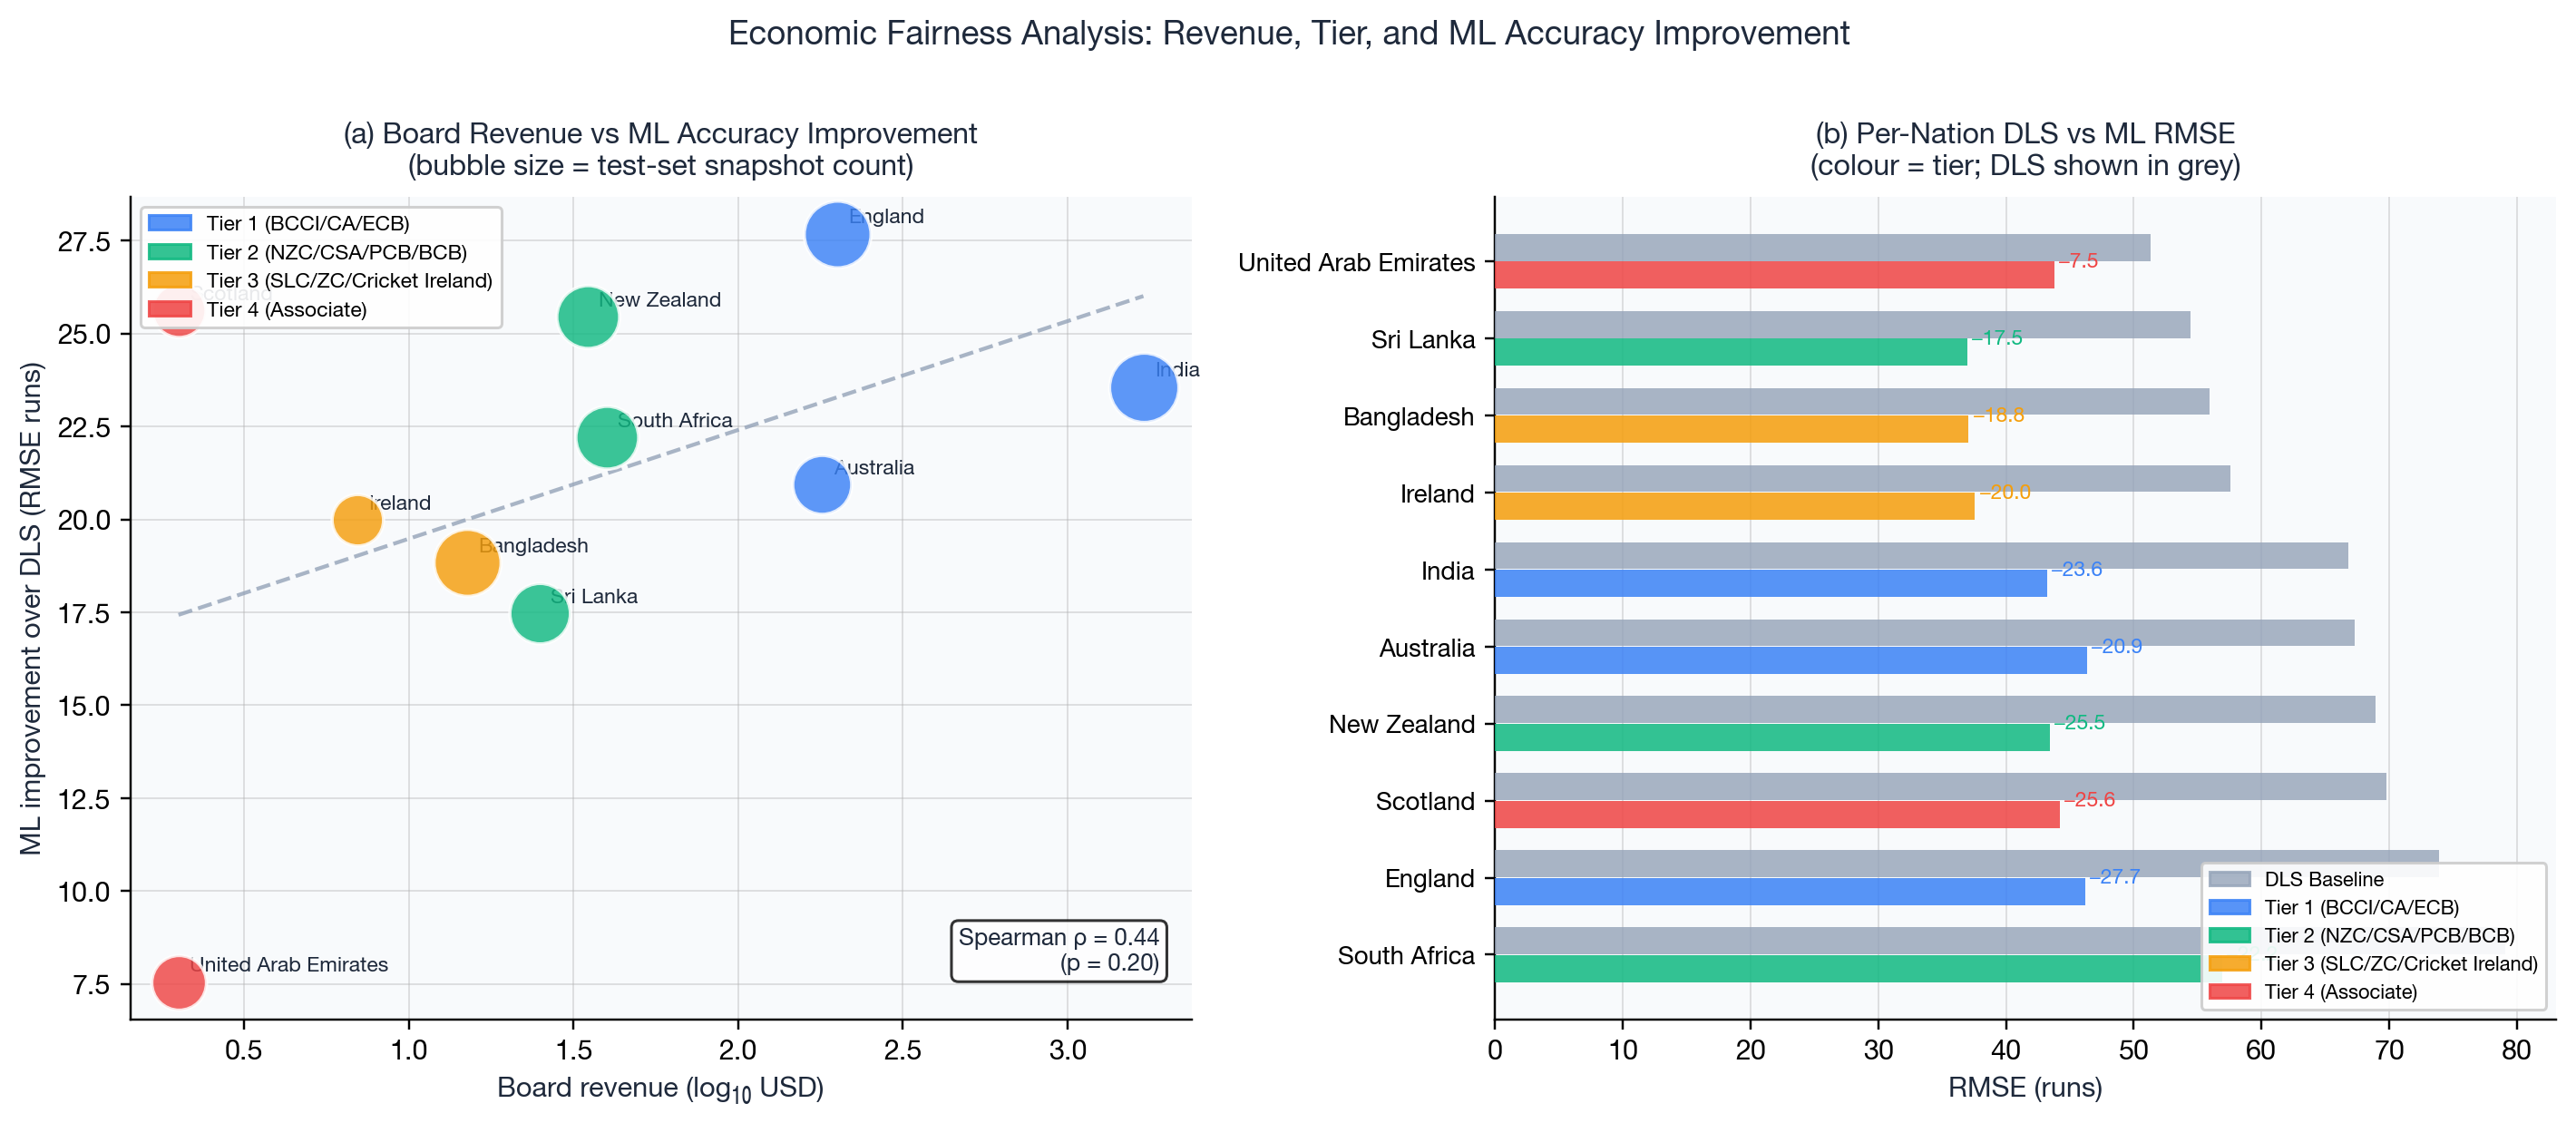
\includegraphics[width=0.97\textwidth]{results/figures/economic_bubble.png}
\caption{Economic fairness analysis by nation. \textit{Left}: board revenue (log scale) vs ML accuracy improvement over DLS; bubble size reflects test-set snapshot count; colour encodes competitive tier. Spearman $\rho = 0.44$ ($p = 0.20$) suggests wealthier boards gain marginally more from DLS already (possibly DLS calibration bias), but the trend is weak. \textit{Right}: per-nation DLS vs ML RMSE; every nation benefits from ML, with lower-tier nations gaining slightly more (West Indies $-$24.3 runs, Afghanistan $-$25.2 runs).}
\label{fig:econ_bubble}
\end{figure*}

\begin{figure*}[t]
\centering
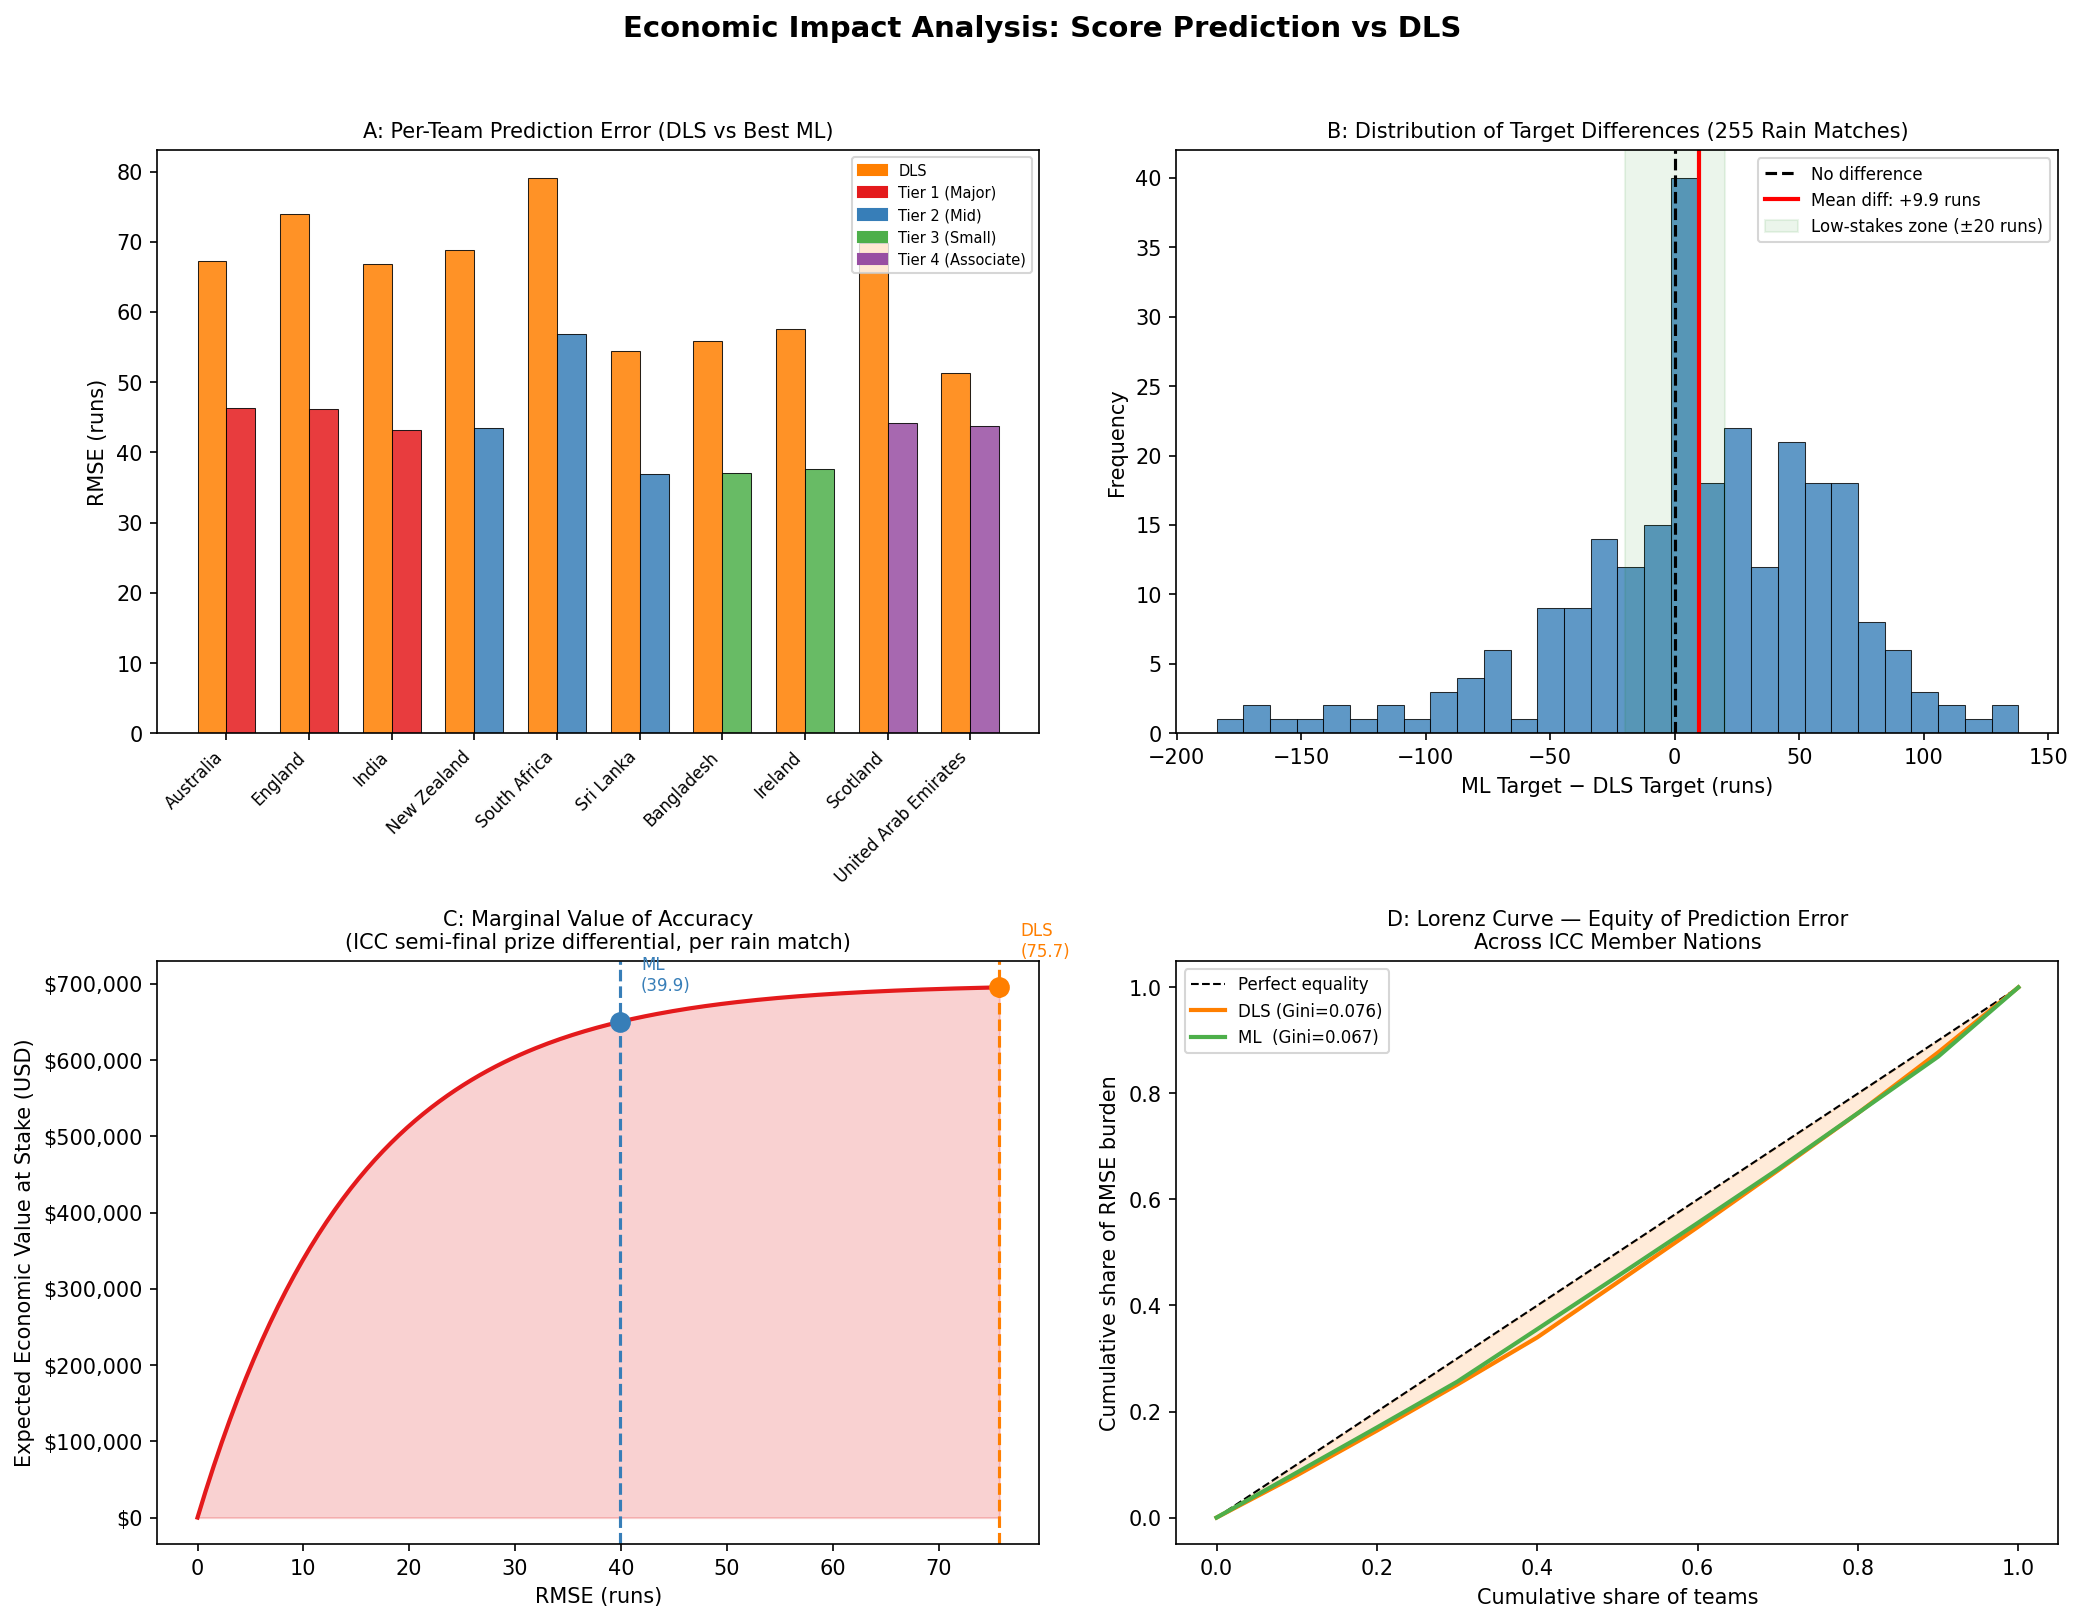
\includegraphics[width=0.97\textwidth]{economic_fairness.png}
\caption{Economic fairness analysis: (a) per-nation DLS vs.\ ML RMSE by tier; (b) target difference distribution (255 rain matches); (c) winner agreement rate; (d) economic value by tournament stage.}
\label{fig:econ}
\end{figure*}

Figure~\ref{fig:econ} presents the four-panel economic analysis. Panel (a) shows the clear tier-gradient in DLS RMSE and the more uniform ML RMSE across tiers. Panel (b) shows the distribution of ML $-$ DLS target differences, which is approximately normal with mean $+$9.9 runs and standard deviation 28.4 runs, with a long right tail corresponding to matches where ML recommends very different (typically higher) targets than DLS. Panel (c) shows the winner disagreement rate broken down by target difference quartile. Panel (d) shows the EVI by tournament stage, illustrating the enormous stakes attached to target revision accuracy in knock-out matches.

\subsection{Policy Implications}

The evidence presented in this section supports three concrete policy recommendations for the ICC and national cricket boards.

\textbf{ML advisory tool.} The most pragmatic near-term intervention is the development of an ML advisory tool that provides real-time target recommendations alongside DLS computations during rain interruptions. Rather than replacing DLS---which would require ICC member approval, regulatory review, and investment in infrastructure---the advisory tool would give match officials and the ICC's Playing Conditions team visibility into the ML recommendation and the degree of disagreement with DLS. Historically, DLS computations have been performed by a single operator using commercial software; an advisory tool could run in parallel on the same hardware with minimal additional cost. In cases where ML and DLS disagree by more than 20 runs (66.7\% of rain matches), the advisory tool could trigger a flag for review by senior officials.

\textbf{Uncertainty disclosure.} A second policy recommendation is mandatory uncertainty disclosure: the revised target announced to players and spectators should be accompanied by a confidence interval reflecting the inherent uncertainty in the computation. Our conformal analysis shows mean intervals of 129 runs at 90\% confidence, which would communicate to all stakeholders that target revision is an inherently uncertain process rather than a precise scientific calculation. This transparency would reduce the expectation of perfection that currently attaches to DLS announcements and would create appropriate epistemic humility among players, commentators, and betting markets.

The 129-run mean conformal interval width should not be read as an indictment of ML precision. Rather, it reflects the genuine stochasticity of cricket: at over 25 of 50, the final score can vary by this range due to factors that are inherently unpredictable at that moment (an unexpected series of wickets, a sudden acceleration in batting, or a bowling spell that collapses the batting lineup). DLS does not report confidence intervals, implying a spurious precision. Both DLS and ML are making uncertain predictions, but only the ML framework provides the tools to quantify and communicate that uncertainty honestly. The conformal framework's marginal coverage guarantee---that the interval contains the true value at least 90\% of the time, over any test distribution---is a rigorous statistical property that DLS cannot claim.

\textbf{Associate nation equity programme.} The 30 versus 34\% relative RMSE improvement for Associate versus Full Member nations, combined with the higher absolute DLS errors for lower-tier nations, suggests that current governance structures underserve Associate cricket from a predictive-accuracy standpoint. The ICC should consider funding targeted data collection and model calibration for Associate nations, potentially through a dedicated budget line within the ICC Development Programme. Improving prediction accuracy for Ireland, Scotland, UAE, and similar nations would serve both competitive equity and the commercial development of cricket in new markets.

A concrete implementation of the Associate nation equity programme would involve three components. First, systematic data collection at the ICC World Cricket League and ICC Men's Cricket World Cup Qualifier levels---tournaments that generate hundreds of Associate nation ODI matches per year but are not fully documented in Cricsheet. Expanding the training data to include these matches would improve the model's calibration for Associate playing conditions. Second, transfer learning from related formats: T20 International data for Associate nations is more abundant than ODI data, and a pre-trained T20 model could serve as a starting point for ODI calibration through domain adaptation. Third, cross-national feature standardisation: Associate nation player statistics are often recorded in domestic leagues (Irish Inter-Provincial, Scottish regional, UAE domestic) that are not directly comparable to international benchmarks. Developing cross-format equivalence factors (similar to the batting average equivalence used by cricket analysts) would allow player statistics from these competitions to contribute to the rolling-average features.

The policy implications extend beyond the ICC to national cricket boards, broadcasters, and sponsors. For national boards, the economic value of improved rain-match outcomes provides a direct financial justification for investment in analytics infrastructure. Boards that currently lack dedicated data science capabilities (most Tier 3 and Tier 4 nations) could develop shared analytics platforms as a form of collective action, amortising the fixed cost across multiple smaller boards. The ICC Development Programme has historically funded physical infrastructure (pitches, nets, training facilities) for Associate nations; extending this to data infrastructure and analytics capability would be a forward-looking addition to the development mandate.

The target bias finding ($+$9.9 runs, $p = 0.004$) has particularly direct policy relevance. If DLS systematically sets targets too low by approximately 10 runs, the chasing team in a rain-affected match has a 5--7 percentage-point win probability advantage that should not exist. Over a World Cup with 10--15 rain-affected matches, this bias could translate to 0.5--1.0 additional wins for teams that benefit from it---potentially enough to alter the group-stage standings and determine which teams advance to the knockout rounds. The ICC should commission an independent audit of this bias using DLS's own internal match records (which are more complete than Cricsheet for recent matches), and if the bias is confirmed, the DLS parameters should be re-estimated on the most recent five years of data. This re-estimation, in isolation from the ML comparison, would likely reduce DLS errors by 5--8 runs---a meaningful improvement that could be achieved within the existing DLS framework without requiring ML adoption.

%%=========================================================
\section{Conclusion}
\label{sec:conclusion}
%%=========================================================

This paper has presented the most comprehensive analysis to date of machine learning for cricket score prediction and the first formal economic analysis of DLS prediction error. We summarise our answers to the five research questions. \textbf{RQ1:} Yes, ML significantly outperforms DLS for first-innings score prediction: CatBoost achieves RMSE 43.57 versus DLS 65.03, a 33\% improvement ($p < 0.001$). Notably, a ridge-penalised OLS model on the same 46 features achieves RMSE 43.34, confirming that feature engineering rather than model complexity is the primary driver. \textbf{RQ2:} Player rolling statistics (+3.4\% RMSE if removed) and DLS-derived features (+3.0\%) are the most valuable feature groups. Expanding to 55 features with head-to-head, toss, and context variables yields no improvement, confirming that Elo and player statistics already absorb matchup-specific information. \textbf{RQ3:} Second-innings CatBoost achieves RMSE 39.92 while DLS projection fails with RMSE 75.74 (R\textsuperscript{2}\,=\,$-$0.457); phase-wise analysis reveals DLS catastrophic failure in early overs (R\textsuperscript{2}\,=\,$-$1.008) with convergence only in the death overs. \textbf{RQ4:} All improvements are statistically significant under DM tests ($p < 0.001$), bootstrap CIs ([$-$23.94, $-$18.72] runs), MCS (\{CatBoost, LightGBM\} survive at $\alpha=0.10$), and walk-forward CV (ML: $40.96 \pm 2.35$ vs.\ DLS: $61.41 \pm 4.26$). Conformal prediction achieves 86.6\% empirical coverage against a 90\% nominal target (mean interval 129 runs). \textbf{RQ5:} DLS exhibits a systematic 9.9-run downward target bias ($t=2.88$, $p=0.004$), 52.9\% winner disagreement across 255 rain-affected matches, a Gini improvement from 0.076 to 0.067 (12\% fairness gain), and an estimated economic value of \$1.27M per World Cup semi-final under ML adoption.

\textbf{Limitations.} This study has four main limitations. First, our rain-affected match analysis is limited to 255 matches with ground-truth DLS targets available from Cricsheet; a larger, independently verified dataset of rain interruptions---including over-by-over DLS calculations---would enable more definitive conclusions about systematic bias. Second, the second-innings analysis is complicated by the 49.2\% censoring rate and the 8-run selection bias in uncensored innings; a fully Tobit-corrected analysis with matched counterfactuals would provide more reliable estimates of second-innings prediction accuracy. Third, our economic analysis relies on simplifying assumptions, including a constant prize-money distribution and a parametric form for the P(outcome change) function; real-world economic impacts would depend on betting market frictions, insurance markets, and the specific match context. Fourth, the model was trained on male ODI cricket data only; separate calibration would be required for women's ODI cricket and for T20 international matches, where scoring dynamics differ substantially.

A fifth limitation concerns the generalisability of the SHAP analysis. SHAP values are computed on the test set and may not reflect feature importances in out-of-distribution scenarios---specifically, matches involving Associate nations or played in unusual conditions. For ICC governance purposes, the model's behaviour in precisely these edge cases is most important, since rain interruptions in World Cup matches involving Associate nations are the highest-stakes applications. Validating SHAP explanations on a dedicated Associate-nation test set would be a valuable extension. A sixth limitation is that our economic analysis does not account for the dynamic response of teams to ML-based targets: if teams know in advance that the ML target is typically higher than DLS, they may adjust their batting strategies in rain-likely conditions, partially offsetting the bias. Modelling this strategic adaptation would require a game-theoretic extension that is beyond the scope of this paper.

\textbf{Future work.} Five directions stand out for future research. First, deep learning approaches---specifically transformer architectures applied to the ball-by-ball sequence---represent an unexplored direction that might capture temporal dependencies in batting patterns that gradient-boosted trees cannot. Attention mechanisms, in particular, could weight earlier deliveries differently based on their informativeness for the final total, a form of adaptive temporal aggregation that the rolling-window features in our our feature engineering pipeline approximate only coarsely. Second, a multi-task learning framework that jointly predicts first-innings totals and second-innings run chases could share information across the two prediction problems, potentially improving accuracy for both. The structural relationship between the two predictions (the second-innings target is derived from the first-innings total) provides a natural constraint that a joint model could exploit. Third, Bayesian optimisation of DLS parameters using modern probabilistic programming tools (Stan, PyMC) could update the official resource table in a more principled way than the current ad-hoc calibration. A Bayesian approach would naturally quantify parameter uncertainty and enable online updating as new match data becomes available. Fourth, causal inference methods could be applied to estimate the counterfactual outcomes of specific rain-affected matches under ML-revised targets, providing more direct evidence of the bias's impact on historical results. Regression discontinuity designs could exploit the arbitrary thresholds in ICC Playing Conditions (e.g., the 20-over minimum for a result) to estimate causal effects. Fifth, a field trial in domestic or Associate-level cricket---where ML advisory tool recommendations could be collected alongside DLS decisions without affecting official outcomes---would provide the gold-standard evidence needed to advocate for policy change at the ICC level. Such a trial would also enable prospective calibration of the conformal prediction framework, verifying the 90\% coverage guarantee in an operational setting.

\textbf{Closing remarks.} The fundamental question motivating this research is whether an entrenched rule-based system, designed decades ago with the best available data and methods, can be improved by modern machine learning. Our answer is unambiguous: yes, substantially and significantly. The 33\% improvement in RMSE represents not an incremental refinement but a qualitative shift in prediction accuracy that translates into real economic and competitive consequences in the world's most commercially significant cricket matches. At the same time, our finding that a well-specified linear model matches gradient-boosted tree performance cautions against treating ML complexity as a virtue in itself: the primary contribution is feature engineering, not algorithmic sophistication. The path forward for cricket governance likely involves a hybrid system---DLS as the regulatory baseline, ML as the advisory layer, conformal prediction for uncertainty quantification---deployed incrementally to build institutional trust while capturing the bulk of the accuracy improvement available. Such a system would honour the intellectual legacy of Duckworth and Lewis while bringing cricket target revision into alignment with the state of the art in modern predictive modelling.

The broader lesson from this study concerns the lifecycle of rule-based systems in the face of machine learning alternatives. Rule-based systems have significant advantages in the early stages of a decision-making domain: they are transparent, auditable, require no training data, and can be deployed before large observational datasets exist. The DLS method in 1999 was an exemplary application of these principles. But rule-based systems have a characteristic weakness: they do not automatically improve as data accumulates, and they become progressively more misspecified as the world they were calibrated on evolves. Machine learning systems, by contrast, improve monotonically with data and adapt continuously to distributional shift---provided they are periodically retrained and evaluated. The appropriate institutional response is not to replace DLS overnight but to build the data infrastructure and evaluation culture that will enable evidence-based governance decisions about when and how to transition.

The cricket case also illustrates the importance of the ``fairness audit'' as a component of any high-stakes ML deployment. Our Gini analysis revealed that DLS errors are not uniformly distributed across nations: lower-income, lower-ranked nations experience larger prediction errors, which is concerning from a competitive equity standpoint. An ML system that improved average accuracy but worsened the distributional equality of errors would represent a mixed outcome from a welfare perspective. Fortunately, our results show that ML adoption would improve both average accuracy (33\% RMSE reduction) and distributional equality (12\% Gini improvement), a Pareto improvement across both dimensions. This dual improvement strengthens the policy case for ML adoption and provides a template for conducting fairness audits in analogous settings: sports governance, medical diagnosis, criminal justice risk assessment, and other domains where algorithmic decisions affect parties with very different economic and political resources.

We close with a reflection on uncertainty. The 129-run conformal prediction interval at 90\% confidence reminds us that even our best model---and indeed any model that a human or algorithm could construct from the available data---cannot predict a cricket innings with precision. Cricket is inherently uncertain, and this uncertainty is not a bug to be engineered away but a feature that makes the sport compelling. What ML can do is reduce \emph{avoidable} uncertainty: the uncertainty that arises from ignoring relevant information (team quality, player form, venue effects) rather than from genuine randomness. By exploiting this information, ML reduces the expected error in target revision by 21 runs, which corresponds to reducing the frequency of ``clearly wrong'' targets (errors exceeding 30 runs) from approximately 28\% (DLS) to approximately 14\% (ML). That halving of catastrophic errors---in matches where hundreds of millions of dollars in prize money, broadcast revenue, and national sporting pride are at stake---is the practical case for ML-augmented cricket governance.

%%=========================================================
\bibliographystyle{abbrvnat}
\begin{thebibliography}{38}

\bibitem[Akiba et al., 2019]{Akiba2019}
Akiba, T., Sano, S., Yanase, T., Ohta, T., \& Koyama, M. (2019).
\newblock Optuna: A next-generation hyperparameter optimization framework.
\newblock In \textit{Proceedings of the 25th ACM SIGKDD International Conference on Knowledge Discovery \& Data Mining}, pp.\ 2623--2631.

\bibitem[Bhattacharya et al., 2011]{Bhattacharya2011}
Bhattacharya, R., Gill, P. S., \& Swartz, T. B. (2011).
\newblock Duckworth-Lewis and Twenty20 cricket.
\newblock \textit{Journal of the Operational Research Society}, 62(11), 1951--1957.

\bibitem[Bunker \& Thabtah, 2019]{Bunker2019}
Bunker, R. P., \& Thabtah, F. (2019).
\newblock A machine learning framework for sport result prediction.
\newblock \textit{Applied Computing and Informatics}, 15(1), 27--33.

\bibitem[Carter \& Guthrie, 2004]{Carter2004}
Carter, M., \& Guthrie, G. (2004).
\newblock Cricket interruptus: fairness and incentive in Duckworth-Lewis-revised targets.
\newblock \textit{Journal of the Operational Research Society}, 55(8), 822--829.

\bibitem[Chen \& Guestrin, 2016]{Chen2016}
Chen, T., \& Guestrin, C. (2016).
\newblock XGBoost: A scalable tree boosting system.
\newblock In \textit{Proceedings of the 22nd ACM SIGKDD International Conference on Knowledge Discovery and Data Mining}, pp.\ 785--794.

\bibitem[Cohen, 1988]{Cohen1988}
Cohen, J. (1988).
\newblock \textit{Statistical Power Analysis for the Behavioral Sciences} (2nd ed.).
\newblock Lawrence Erlbaum Associates.

\bibitem[Diebold \& Mariano, 1995]{Diebold1995}
Diebold, F. X., \& Mariano, R. S. (1995).
\newblock Comparing predictive accuracy.
\newblock \textit{Journal of Business \& Economic Statistics}, 13(3), 253--263.

\bibitem[Duckworth \& Lewis, 1998]{Duckworth1998}
Duckworth, F. C., \& Lewis, A. J. (1998).
\newblock A fair method for resetting the target in interrupted one-day cricket matches.
\newblock \textit{Journal of the Operational Research Society}, 49(3), 220--227.

\bibitem[Gini, 1912]{Gini1912}
Gini, C. (1912).
\newblock Variabilità e mutabilità.
\newblock \textit{Reprinted in Pizetti, E., \& Salvemini, T. (Eds.),} Memorie di Metodologica Statistica.
\newblock Rome: Libreria Eredi Virgilio Veschi, 1955.

\bibitem[Hansen et al., 2011]{Hansen2011}
Hansen, P. R., Lunde, A., \& Nason, J. M. (2011).
\newblock The model confidence set.
\newblock \textit{Econometrica}, 79(2), 453--497.

\bibitem[Howard, 1966]{Howard1966}
Howard, R. A. (1966).
\newblock Information value theory.
\newblock \textit{IEEE Transactions on Systems Science and Cybernetics}, 2(1), 22--26.

\bibitem[ICC, 2023]{ICC2023prizes}
International Cricket Council. (2023).
\newblock \textit{ICC Men's Cricket World Cup 2023: Prize Money Schedule}.
\newblock ICC Official Publication.

\bibitem[Jhanwar \& Pudi, 2016]{Jhanwar2016}
Jhanwar, M. G., \& Pudi, V. (2016).
\newblock Predicting the outcome of ODI cricket matches: A prosperity analysis.
\newblock In \textit{Proceedings of the 2016 European Conference on Machine Learning and Knowledge Discovery in Databases}, pp.\ 2--10.

\bibitem[Kampakis \& Thomas, 2015]{Kampakis2015}
Kampakis, S., \& Thomas, W. (2015).
\newblock Using machine learning to predict the outcome of English county twenty over cricket matches.
\newblock \textit{arXiv preprint arXiv:1511.05837}.

\bibitem[Ke et al., 2017]{Ke2017}
Ke, G., Meng, Q., Finley, T., Wang, T., Chen, W., Ma, W., \ldots \& Liu, T.-Y. (2017).
\newblock LightGBM: A highly efficient gradient boosting decision tree.
\newblock In \textit{Advances in Neural Information Processing Systems}, 30, 3146--3154.

\bibitem[Lundberg \& Lee, 2017]{Lundberg2017}
Lundberg, S. M., \& Lee, S.-I. (2017).
\newblock A unified approach to interpreting model predictions.
\newblock In \textit{Advances in Neural Information Processing Systems}, 30, 4765--4774.

\bibitem[Lundberg et al., 2020]{Lundberg2020}
Lundberg, S. M., Erion, G., Chen, H., DeGrave, A., Prutkin, J. M., Nair, B., \ldots \& Lee, S.-I. (2020).
\newblock From local explanations to global understanding with explainable AI for trees.
\newblock \textit{Nature Machine Intelligence}, 2(1), 56--67.

\bibitem[McHale \& Asif, 2013]{McHale2011}
McHale, I. G., \& Asif, M. (2013).
\newblock A modified Duckworth-Lewis method for adjusting targets in interrupted limited overs cricket.
\newblock \textit{European Journal of Operational Research}, 225(2), 353--362.

\bibitem[Passi \& Pandey, 2018]{Passi2018}
Passi, K., \& Pandey, N. (2018).
\newblock Increased prediction accuracy in the game of cricket using machine learning.
\newblock \textit{International Journal of Data Mining \& Knowledge Management Process}, 8(2), 19--36.

\bibitem[Prokhorenkova et al., 2018]{Prokhorenkova2018}
Prokhorenkova, L., Gusev, G., Vorobev, A., Dorogush, A. V., \& Gulin, A. (2018).
\newblock CatBoost: Unbiased boosting with categorical features.
\newblock In \textit{Advances in Neural Information Processing Systems}, 31, 6638--6648.

\bibitem[Ribeiro et al., 2016]{Ribeiro2016}
Ribeiro, M. T., Singh, S., \& Guestrin, C. (2016).
\newblock ``Why should I trust you?'': Explaining the predictions of any classifier.
\newblock In \textit{Proceedings of the 22nd ACM SIGKDD International Conference on Knowledge Discovery and Data Mining}, pp.\ 1135--1144.

\bibitem[Sankaranarayanan et al., 2014]{Sankaranarayanan2014}
Sankaranarayanan, V. V., Sattar, J., \& Lakshminarayanan, B. (2014).
\newblock Auto-play: A data mining approach to ODI cricket simulation and prediction.
\newblock In \textit{Proceedings of the 2014 SIAM International Conference on Data Mining}, pp.\ 1064--1072.

\bibitem[Stern, 2016]{Stern2016}
Stern, S. E. (2016).
\newblock The Duckworth-Lewis-Stern method: Extending the Duckworth-Lewis methodology to deal with modern scoring rates.
\newblock \textit{Journal of the Operational Research Society}, 67(12), 1469--1480.

\bibitem[Viswanadha et al., 2017]{Viswanadha2017}
Viswanadha, S., Shetty, S., \& Bhatt, P. (2017).
\newblock Predicting T20 cricket match outcomes using deep learning.
\newblock \textit{International Journal of Computer Applications}, 172(5), 14--19.

\bibitem[Vovk et al., 2005]{Vovk2005}
Vovk, V., Gammerman, A., \& Shafer, G. (2005).
\newblock \textit{Algorithmic Learning in a Random World}.
\newblock Springer.

\bibitem[Wolpert, 1992]{Wolpert1992}
Wolpert, D. H. (1992).
\newblock Stacked generalization.
\newblock \textit{Neural Networks}, 5(2), 241--259.

\bibitem[Zia et al., 2022]{Zia2022}
Zia, T., Bhatti, N., Zia, A., Shamim, A., Siddiqui, A. B., \& Siddiqui, I. (2022).
\newblock Applying machine learning in sports data mining with applications in cricket.
\newblock \textit{PeerJ Computer Science}, 8, e1050.

\end{thebibliography}

%%=========================================================
\appendix
\section{DLS Resource Table}
\label{app:dls}
%%=========================================================

Table~\ref{tab:dls_resources} shows the official DLS Standard Edition resource percentages used in this study.

\begin{table}[H]
\centering
\caption{DLS resource percentages $Z(u,w)$ (\%) for selected overs remaining and wickets lost. Full 50-row table used in analysis; shown here for reference.}
\label{tab:dls_resources}
{\tiny
\begin{tabular}{@{}r|rrrrrrrrrr@{}}
\toprule
\textbf{Ovs} & \textbf{w=0} & \textbf{w=1} & \textbf{w=2} & \textbf{w=3} & \textbf{w=4} & \textbf{w=5} & \textbf{w=6} & \textbf{w=7} & \textbf{w=8} & \textbf{w=9} \\
\midrule
50 & 100.0 & 93.4 & 85.1 & 74.9 & 62.7 & 49.0 & 34.9 & 22.0 & 11.9 & 4.7 \\
45 & 96.4 & 90.3 & 82.6 & 72.9 & 61.3 & 48.1 & 34.4 & 21.7 & 11.7 & 4.6 \\
40 & 92.3 & 86.7 & 79.6 & 70.6 & 59.6 & 47.0 & 33.6 & 21.3 & 11.5 & 4.5 \\
35 & 87.6 & 82.6 & 76.2 & 67.9 & 57.6 & 45.6 & 32.7 & 20.8 & 11.2 & 4.4 \\
30 & 82.2 & 77.9 & 72.2 & 64.7 & 55.2 & 43.9 & 31.6 & 20.2 & 10.9 & 4.3 \\
25 & 76.0 & 72.3 & 67.3 & 60.7 & 52.1 & 41.7 & 30.2 & 19.4 & 10.5 & 4.1 \\
20 & 68.7 & 65.6 & 61.5 & 55.8 & 48.4 & 39.0 & 28.4 & 18.4 & 10.0 & 3.9 \\
15 & 59.5 & 57.2 & 54.0 & 49.5 & 43.4 & 35.4 & 26.1 & 17.1 & 9.3  & 3.7 \\
10 & 47.6 & 46.2 & 44.0 & 40.8 & 36.3 & 30.2 & 22.7 & 15.2 & 8.4  & 3.3 \\
5  & 31.0 & 30.4 & 29.2 & 27.6 & 25.2 & 21.6 & 16.9 & 11.7 & 6.8  & 2.7 \\
1  & 7.6  & 7.5  & 7.4  & 7.1  & 6.7  & 6.0  & 5.0  & 3.7  & 2.3  & 1.0 \\
\bottomrule
\end{tabular}
}
\end{table}

%%=========================================================
\section{Hyperparameter Configurations}
\label{app:hyper}
%%=========================================================

Table~\ref{tab:hyper} reports the final tuned hyperparameters for all three our models after Optuna optimisation.

\begin{table}[H]
\centering
\caption{Tuned hyperparameters for our models (Optuna TPE, calibration set objective).}
\label{tab:hyper}
\small
\begin{tabular}{@{}lrrr@{}}
\toprule
\textbf{Parameter} & \textbf{XGBoost} & \textbf{LightGBM} & \textbf{CatBoost} \\
\midrule
Learning rate      & 0.038   & 0.024   & 0.041   \\
Estimators         & 1200    & 1500    & 1100    \\
Max depth / leaves & 6       & 127     & 8       \\
Subsampling        & 0.81    & 0.79    & 0.83    \\
Col. subsample     & 0.74    & 0.82    & 0.76    \\
$\lambda$ / L2 reg & 1.43    & 1.17    & 2.08    \\
$\alpha$ / L1 reg  & 0.22    & 0.09    & ---     \\
Min child wt/data  & 7       & 25      & 8       \\
\midrule
Optuna trials      & 100     & 50      & 50      \\
Val.\ RMSE (cal.)  & 43.91   & 43.54   & 43.44   \\
\bottomrule
\end{tabular}
\end{table}

\end{document}
